\documentclass[11pt,a4paper,oneside]{report}
\usepackage[a4paper,top=27mm,bottom=27mm,left=28mm,right=25mm]{geometry}
\usepackage[T1]{fontenc}
\usepackage[utf8]{inputenc}
\usepackage{lmodern,microtype}
\usepackage{amsmath,amssymb,amsthm,mathtools,bm}
\usepackage{graphicx,booktabs,multirow,longtable,threeparttable,array}
\usepackage{caption,subcaption,enumitem,xcolor}
\usepackage{tikz}
\usetikzlibrary{arrows.meta,positioning,calc}
\usepackage[authoryear,round]{natbib}
\usepackage{tocbibind}
\usepackage[titletoc]{appendix}
\usepackage{fancyhdr,setspace,placeins,flafter,float}
\usepackage[hidelinks]{hyperref}
\usepackage{url}
\graphicspath{{figures/}}
\setstretch{1.25}
\setlength{\parskip}{0.35em}
\setlength{\headheight}{16pt}
\setlength{\emergencystretch}{2em}
\setcounter{tocdepth}{1}
\setlist{nosep,leftmargin=*}
\captionsetup{font=small,labelfont=bf,width=\textwidth}
\pagestyle{fancy}
\fancyhf{}
\fancyhead[L]{\small\nouppercase{\leftmark}}
\fancyhead[R]{\small\thepage}
\renewcommand{\headrulewidth}{0.3pt}
\fancypagestyle{plain}{\fancyhf{}\fancyfoot[C]{\small\thepage}\renewcommand{\headrulewidth}{0pt}}
\theoremstyle{plain}
\newtheorem{theorem}{Theorem}[chapter]
\newtheorem{lemma}[theorem]{Lemma}
\newtheorem{proposition}[theorem]{Proposition}
\newtheorem{corollary}[theorem]{Corollary}
\theoremstyle{definition}
\newtheorem{assumption}[theorem]{Assumption}
\newtheorem{definition}[theorem]{Definition}
\theoremstyle{remark}
\newtheorem{remark}[theorem]{Remark}
\newcommand{\E}{\mathbb{E}}
\renewcommand{\Pr}{\mathbb{P}}
\newcommand{\R}{\mathbb{R}}
\newcommand{\ind}{\mathbf{1}}
\newcommand{\MCB}{\mathrm{MCB}}
\newcommand{\VaR}{\mathrm{VaR}}
\newcommand{\ES}{\mathrm{ES}}
\newcommand{\cC}{\mathcal{C}}
\newcommand{\cF}{\mathcal{F}}
\newcommand{\Var}{\mathrm{Var}}
\newcommand{\code}[1]{\texttt{#1}}
\newcommand{\rulename}[1]{\textsc{#1}}
\hypersetup{pdftitle={VolPFN: Volatility Forecasting from a Synthetic Prior},pdfauthor={Bader Matar},pdfsubject={MSc dissertation in Artificial Intelligence}}
\begin{document}
\pagenumbering{roman}
\hypersetup{pageanchor=false}
\begin{titlepage}
\centering
{\large University of Sheffield\par}
\vspace{0.25cm}
{\normalsize Department of Computer Science\par}
\vspace{3cm}
{\LARGE\bfseries VolPFN: Volatility Forecasting\par}
\vspace{0.35cm}
{\LARGE\bfseries from a Synthetic Prior\par}
\vspace{1cm}
{\large Performance, prior attribution and tail recalibration\par}
\vspace{2.8cm}
{\Large Bader Matar\par}
\vspace{0.7cm}
{\normalsize MSc in Artificial Intelligence\par}
\vspace{1.1cm}
{\normalsize Supervisor: Georgios Moulantzikos\par}
\vspace{0.7cm}
{\normalsize Registration number: \rule{3cm}{0.4pt}\par}
\vfill
{\normalsize Dissertation submitted for the MSc in Artificial Intelligence\par}
\vspace{0.3cm}
{\normalsize September 2026\par}
\vspace{0.3cm}
{\footnotesize Research revision: 2 October 2026; Stage 4 editorial cleanup: 3 October 2026\par}
\end{titlepage}
\hypersetup{pageanchor=true}

\chapter*{Declaration}
\addcontentsline{toc}{chapter}{Declaration}
All sentences or passages quoted in this report from other people's work have been specifically acknowledged by clear cross-referencing to author, work and page(s). Any illustrations that are not the work of the author of this report have been used with the explicit permission of the originator and are specifically acknowledged. I understand that failure to do this amounts to plagiarism and will be considered grounds for failure in this project and the degree examination as a whole.

\vspace{1.5cm}
\noindent Name: Bader Matar

\vspace{0.8cm}
\noindent Signature:

\vspace{0.8cm}
\noindent Date:



\chapter*{Abstract}
\addcontentsline{toc}{chapter}{Abstract}
Financial volatility changes over time, while short market histories provide limited examples for learning. We develop VolPFN, a neural forecaster trained on simulated returns, to examine what synthetic training contributes to market prediction. Its weights remain fixed during use; calibration and forecast combinations are fitted separately.

The main experiment matches architecture, initial weights and training allocation across simulation designs. Broad training improves the common log score by about 0.0052 nats per return, with an interval supporting a positive gain. The improvement is modest and concentrated in a few markets. It supports the combined design without identifying an individual causal ingredient.

VolPFN leads the tested general pretrained benchmark, and its variants lead the daily-return-only leaderboard. These rankings evaluate complete procedures without establishing adjusted superiority over every competitor. Distribution prediction outperforms direct risk prediction, while extra volatility supervision has no detected benefit. Regularisation and development selection make historical training competitive. A daily--intraday blend improves on calibrating the intraday model alone, with stronger alternatives unresolved. On fixed exchange-traded funds, synthetic training without extra supervision improves on the historical procedure, but superiority over the rolling financial benchmark remains inconclusive.

A compact fitted rule retains much of an earlier network's scale advantage without explaining its computation. Residual correction helps most clearly with Gaussian tails. Additional neural joint-score gains remain uncertain, and the fixed correction rule sometimes loses to filtered historical simulation.

The evidence therefore supports useful prediction within defined comparisons. Prior data exposure, shared shocks and uncertainty conditional on saved forecasts limit generalisation.

\chapter*{Acknowledgements}
\addcontentsline{toc}{chapter}{Acknowledgements}
I thank Georgios Moulantzikos for his supervision and the Kuwait government scholarship programme for supporting my studies. I also thank the researchers who provided the Oxford-Man data and the replication material used in this project.

\chapter*{Abbreviations and reading guide}
\addcontentsline{toc}{chapter}{Abbreviations and reading guide}
The reading guide assumes familiarity with averages and graphs without prior knowledge of financial volatility or prior-fitted networks. Chapter~\ref{ch:background} introduces the financial and machine-learning concepts needed for the experiments. The appendices retain the detailed implementation specifications and supporting results.

\begingroup
\small
\begin{longtable}{@{}>{\raggedright\arraybackslash}p{2.7cm}>{\raggedright\arraybackslash}p{11.0cm}@{}}
\toprule Term & Meaning in this dissertation \\
\midrule\endfirsthead
\toprule Term & Meaning in this dissertation (continued) \\
\midrule\endhead
ARCH / GARCH & Models that update a changing variance from past shocks and, for GARCH, earlier variance estimates. \\
EWMA & Exponentially weighted moving average: gives progressively less weight to older observations. \\
LSTM & Long short-term memory: a recurrent neural architecture used in the daily comparisons. \\
RK & Realised kernel: an estimate of variability within a trading session, used as a proxy or a past input. \\
HAR & Heterogeneous autoregressive model: combines daily, weekly and monthly realised-risk summaries. \\
STES & Smooth-transition exponential smoothing: changes the updating response with observed conditions. \\
GNNHAR & Graph neural HAR: combines realised-risk summaries using links between assets. \\
TTM & Tiny Time Mixers: the pretrained model supplying a forecast from past realised kernels. \\
GINN & GARCH-informed neural network: combines observed innovations and a fitted GARCH teacher. \\
GP & Gaussian process: a probability model over functions. \\
PFN / VolPFN & Prior-data fitted network; VolPFN is the volatility-oriented network developed here. \\
QLIKE & A loss for evaluating positive risk forecasts; smaller values indicate better prediction. \\
RMS & Root-mean-square scale used to normalise returns; the stated centring and observation rules depend on the study. \\
M2 & Expected squared return (the second moment). It equals variance plus squared predictive mean. \\
NLL / nats & Negative log likelihood, with lower values preferred; nats are log-score units using natural logarithms. \\
ETF & Exchange-traded fund: a fund traded on an exchange, used here to extend the evaluated asset population. \\
VaR / ES & Value-at-Risk is a lower-return threshold; Expected Shortfall is the average return below that threshold. \\
FZ0 & A loss that evaluates VaR and ES together; smaller is better. \\
FHS & Filtered historical simulation: estimate a residual distribution after removing scale, then restore forecast scale. \\
CI & Confidence interval: uncertainty under the stated sampling procedure and assumptions. \\
Arm & One experimental configuration; it specifies the model and training procedure being compared. \\
Full / noaux & Full uses extra supervision from simulated volatility labels. Noaux removes that training loss while retaining the same physical output heads. \\
Direct / historical & Direct predicts expected squared return with QLIKE training. Historical learns the return distribution from earlier market windows. \\
Fixed-final & Use the checkpoint saved at the final scheduled update, without choosing it from validation scores. \\
Checkpoint / seed & A checkpoint stores trained weights. A seed sets pseudorandom training choices. \\
TRAIN / development & TRAIN denotes the observations used for fitting. Development observations are used for the stated selection or calibration decisions. \\
Common-$t_8$ / native & Common-$t_8$ evaluates scales under the same Student distribution with eight degrees of freedom. Native scoring evaluates each model's own return distribution. \\
UniVol & The project's non-neural forecast that combines updating risk filters and restart experts. \\
Compact rule / distillation & A small explicit predictor; distillation fits that predictor to imitate network forecasts. Likelihood fitting instead predicts observed returns. \\
Helper / blend & A helper supplies an additional forecast. A blend combines it with the daily forecast using parameters fitted from earlier observations. \\
Scoring mask / key & The mask fixes eligible observations. A key identifies one market and date. \\
Union date / family & A union date occurs in at least one included market. A comparison family is the set of tests adjusted together for multiplicity. \\
Guard / hindsight & The guard follows the study's fixed rule for applying tail correction. Hindsight alternatives use later information and are diagnostic. \\
Oracle / reference & An oracle uses known simulated truth. Other references may also use information unavailable to the evaluated forecaster; their privileges are specified. \\
\bottomrule
\end{longtable}
\endgroup

\begingroup
\setstretch{1}
\tableofcontents
\listoffigures
\begingroup
\small
\listoftables
\endgroup
\endgroup
\clearpage
\pagenumbering{arabic}
\chapter{Introduction}
\label{ch:introduction}

\section{The problem: forecasting uncertainty}

Forecasting a financial return involves estimating how large tomorrow's movement might be as well as its direction. Two forecasts with similar expected returns can carry different levels of risk. To describe this uncertainty, we use \emph{volatility}, the conditional standard deviation of returns, whose square is conditional variance.

We forecast the open-to-close log returns of stock-market indices, which summarise groups of stocks. This target measures movement within a trading session, leaving overnight movement outside the study. Rather than describing uncertainty through one risk value alone, a \emph{predictive distribution} assigns probabilities to possible returns. Its width describes the overall scale of uncertainty, while its tails determine the probabilities of extreme outcomes. Consequently, forecasts with equal variance can still disagree about the likelihood of a severe loss.

An illustrative turbulent week in the S\&P 500 makes this distinction useful. A forecaster needs to assess whether a large movement is an isolated shock or part of a persistent rise in uncertainty. Even if it estimates the overall scale sensibly, it may assign too little probability to severe losses. This illustrative case connects forecasting performance to the assumptions learned during training and the conversion of scale into tail risk. It supplies no additional empirical evidence.

We address these concerns while asking whether a large network can respond to changing market conditions without being repeatedly fitted to each market. The benchmarks assess the usefulness of the resulting forecasts against other procedures, while Chapter~\ref{ch:analysis} tests what simulated training histories contribute. The tail studies then examine whether useful scale forecasts also provide reliable predictions of extreme losses.

\section{The proposed approach and its motivation}

Conventional volatility models learn an updating rule from market histories. For example, GARCH combines recent squared shocks with earlier variance estimates through a relatively inexpensive recursion \citep{bollerslev1986generalized}. These economical procedures provide a benchmark for a more flexible forecaster. Added complexity needs to be justified by forecasting performance.

The approach developed here is VolPFN, a volatility-oriented prior-data fitted network trained on simulated histories. Its \emph{training prior} defines the artificial processes and parameter settings from which those histories are generated. Following the prior-fitted approach of \citet{muller2022transformers}, the network learns to predict a return distribution from the supplied history. During market use, each new history changes the prediction, but the neural weights remain fixed.

Simulation allows us to generate training examples whose underlying volatility is known. However, this is useful only to the extent that the tasks teach an appropriate forecasting rule: omitted market behaviour and irrelevant simulated tasks can both make that rule unsuitable. A benchmark cannot isolate this issue because its competitors also differ in architecture, training data and outputs. We therefore compare two simulation designs with the remaining network settings matched, allowing us to test the contribution of the combined training design.

We also fit a small explicit predictor to examine how much of an earlier network's forecasting advantage can be retained with a simpler rule. Once fitted, the rule uses returns alone and runs independently of the network. Its predictive performance can therefore help assess whether a large model is needed. Similar scores, however, would neither establish shared internal computation nor amount to reverse-engineering the network.

The final part of the argument concerns the conversion from scale to tails. Dividing returns by their forecast scale produces \emph{standardised residuals}, whose empirical distribution can replace an assumed tail shape through filtered historical simulation \citep{baroneadesi1999var}. This can repair unsuitable tails, but estimating them from a short history introduces sampling error. We evaluate both the benefit of correction and the cost of estimating it.

\section{Research questions and contributions}

The overarching question is: \emph{what does a synthetic volatility prior contribute to useful market forecasts, and where does that contribution stop?} We develop this question through six research questions. Two extensions broaden the evaluation in different ways. Exchange-traded funds (ETFs) extend the asset population beyond indices, whereas Tiny Time Mixers (TTM), a pretrained model using past intraday risk measurements, adds information to a forecast. Keeping their roles distinct helps identify what each extension can establish.

\begin{enumerate}[label=RQ\arabic*.,leftmargin=1.5cm]
\item Does VolPFN improve forecasting scores against the specified general and financial benchmarks, including evaluation on a fixed external ETF population?
\item Does the broad simulation design improve prediction relative to a matched Mat\'ern design?
\item What do the component comparisons and a historical model selected using earlier development observations establish about the training procedure?
\item How much of an earlier neural forecast's advantage can a compact rule recover?
\item What changes when daily forecasts are combined with realised-risk information, including comparison with calibration of TTM alone?
\item When does residual tail correction improve forecasts of Value-at-Risk and Expected Shortfall together?
\end{enumerate}

The questions follow the distinction between performance and explanation. RQ1 and RQ5 assess forecasting performance under the information available to each procedure. RQ2--RQ4 examine training choices and whether neural complexity is needed to retain useful prediction. RQ6 then considers whether correcting a scale forecast improves its prediction of extreme-loss risk. Each question requires an appropriate comparison and score, so a single leaderboard cannot answer the whole argument.

The dissertation makes four contributions in the following order:
\begin{enumerate}
\item \textbf{A matched test of prior contribution.} We train five broad--Mat\'ern pairs with architecture, initial weights and training allocation held fixed. The broad design improves the common log score by about 0.0052 nats per return, with positive means in all five pairs and most markets. This supports a contribution from the combined simulation design, while leaving the causal contribution of individual ingredients unresolved.
\item \textbf{A volatility-oriented forecaster and a differentiated evaluation.} VolPFN predicts a heavy-tailed return distribution from past returns. It ranks first in the tested general pretrained benchmark, and its variants lead the daily-return-only leaderboard, which includes dedicated financial models and general pretrained forecasters. These rankings describe the evaluated procedures; adjusted tests do not establish superiority over every competitor. The component comparisons favour distribution prediction over direct prediction of expected squared return and detect no benefit from extra volatility supervision. The improved historical procedure is competitive on indices. The intraday blend improves on the specified TTM-only calibration controls, while fixed ETF evaluation supports the synthetic model without extra supervision over the improved historical procedure. Superiority over rolling GJR and the principal stronger intraday alternatives remains inconclusive.
\item \textbf{Evidence on predictive compression.} Fitting a small rule directly to observed returns retains about 83\% of an earlier network's development advantage over UniVol, the project's non-neural combination of risk filters. We report fits that imitate the network separately, because retaining forecasting performance and faithfully reproducing another predictor answer different questions.
\item \textbf{An evaluation of tail correction and its cost.} Simulations and market comparisons show that residual correction helps selectively, with the clearest benefit for Gaussian tails. Additional neural gains in the joint tail score remain inconclusive, and the fixed rule for applying correction sometimes performs worse than filtered historical simulation.
\end{enumerate}

\section{Organisation and scope}

The chapter sequence develops this argument from concepts to evaluation and interpretation. Chapter~\ref{ch:background} introduces the relevant concepts and literature, followed by the targets, populations and decision rules in Chapter~\ref{ch:data}. Chapter~\ref{ch:forecast} explains VolPFN and evaluates its forecasts. Chapter~\ref{ch:analysis} then examines training choices and the performance retained by a small rule. Chapters~\ref{ch:recalibration} and \ref{ch:tailresults} specify and evaluate residual tail correction, before Chapter~\ref{ch:discussion} brings the answers together.

Our conclusions apply to the recorded markets, dates and forecasting procedures. Section~\ref{sec:exposure} documents prior research contact with the data, which limits the interpretation of the evaluations. The appendices retain implementation details, supporting results and unsuccessful comparisons so that the main argument can remain readable without separating it from the evidence needed to check its scope.
\chapter{Background: from volatility models to reusable forecasters}
\label{ch:background}

To assess VolPFN, we need to connect three ideas: how volatility changes, how a forecasting rule can be reused, and how forecast scale becomes a prediction of extreme losses. This chapter introduces the concepts behind those ideas and the relevant modelling approaches. It also explains why a comparison that establishes useful performance may not identify the source of that performance.

\section{The forecasting objects}
\label{sec:bg-concepts}

The forecast interval determines what is being predicted. An open-to-close log return is the logarithm of closing price divided by opening price and approximates proportional price change for small movements. It measures movement within the session, excluding overnight movement. A close-to-close forecast covers a different interval, so its performance cannot be ranked directly against this target.

We use the term \emph{information set} for the observations available when a forecast is issued. A causal procedure must respect this boundary throughout preprocessing and prediction. For example, normalising a series with observations from its whole history introduces later information, even if the network itself subsequently receives only past observations.

Three related quantities describe the size of uncertain returns. Variance is the expected squared deviation from the conditional mean, volatility is its square root, and the second moment is expected squared return. Variance and second moment coincide under the zero-conditional-mean working model used here. However, one observed squared return remains a noisy proxy for that expectation, rather than a direct observation of it.

Several patterns describe these uncertain movements. \emph{Clustering} places large movements near other large movements; \emph{heavy tails} make extremes more frequent than under a Gaussian law; and \emph{asymmetry} gives equal-sized positive and negative shocks different volatility responses. A predictive \emph{density} assigns probabilities to intervals through its area. These features explain why variance alone cannot specify tail risk.

Tail shape is a separate part of the prediction. In a Student distribution, degrees of freedom control tail thickness, while its scale parameter differs from its standard deviation. A mixture combines densities through non-negative weights that sum to one. Consequently, an improvement in density prediction can come from better scale, better shape, or both; the score alone does not identify which changed.

\section{Persistent variance: ARCH and GARCH}

ARCH describes changing variance through past squared shocks \citep{engle1982arch}. GARCH adds earlier variance estimates, allowing persistent information to be retained with fewer coefficients \citep{bollerslev1986generalized}. Maximum likelihood fits these coefficients by rewarding density assigned to observed returns. Once fitted, the model can update its state without refitting the coefficients. Keeping these operations separate matters when comparing fitting cost and forecasting behaviour.

A variance recursion does not determine the complete return distribution. The same GARCH scale can support Gaussian or Student forecasts, so a density gain may reflect the scale update or the assumed tail law. We therefore use fitted GARCH as an economical benchmark and also compare scale forecasts under a common scoring distribution. The latter comparison holds the scoring law fixed rather than attributing every density difference to volatility prediction.

\section{Asymmetry, hidden states and residual tails}

Several extensions allow behaviour beyond a symmetric variance recursion. EGARCH makes log variance depend on the sign of a shock \citep{nelson1991conditional}, while GJR-GARCH adds a separate response to negative shocks \citep{glosten1993relation}. Stochastic-volatility models give hidden variance its own disturbances \citep{harvey1994multivariate}. Because several hidden paths can explain the same returns, filtering updates beliefs about the hidden state instead of following a single recursion with known parameters.

Bayesian prediction combines parameter assumptions with the likelihood of the observed history, then averages future predictions over posterior uncertainty. Prior-fitted learning aims to approximate this operation through a reusable predictor. Simpler updating methods avoid that inference: RiskMetrics' exponentially weighted moving averages (EWMA), for example, give progressively less weight to older squared returns \citep{riskmetrics1996}.

Filtered historical simulation (FHS) separates changing scale from residual tail shape \citep{baroneadesi1999var}. A return of minus two percent divided by forecast volatility of two percent becomes a residual of minus one. Restoring that residual at one-percent volatility produces a minus-one-percent outcome. Removing and restoring scale in this way allows an empirical residual distribution to replace a fixed tail law. A longer history improves precision under stability, but may adapt slowly when the tails change. The later tail chapters evaluate this established operation and its trade-off.

\section{Realised measurements and multiple horizons}

Intraday observations offer another source of risk information. Realised variance sums intraday squared returns, while related estimators reduce microstructure effects such as bid--ask noise \citep{andersen2003modeling}. These quantities estimate variability over a specified interval. As inputs or evaluation proxies, they measure realised variability over that interval, not tomorrow's conditional variance directly.

The heterogeneous autoregressive model (HAR) combines daily, weekly and monthly realised-risk summaries \citep{corsi2009simple}. Component models distinguish rapid responses from persistent risk \citep{engle1999permanent}, and smooth-transition exponential smoothing (STES) changes responsiveness with observed conditions \citep{taylor2004smooth}. These approaches motivate the multiple return horizons in VolPFN and the compact rules. Their information still differs: HAR uses intraday measurements unavailable to the daily-return model, whereas scoring a daily-return model against a realised measure does not give that model the measure as an input.

\section{Flexible dynamics and reusable inference}

Score-driven models provide an explicit way to adapt parameters using the derivative of log likelihood \citep{creal2013generalized,harvey2013dynamic}. The assumed return distribution controls the response to an extreme observation. This connects the forecast law to state updating and supplies a statistical alternative to learning the shock response through a network.

A Gaussian process (GP) defines a probability distribution over functions through a covariance kernel. Mat\'ern kernels can vary regularity and persistence \citep{rasmussen2006gaussian}. Exponentiating a GP log-variance path produces positive variance without a return-driven GARCH recursion. We use this construction as the alternative simulation design in the matched-prior experiment.

GP methods already provide flexible approaches to volatility. Gaussian Copula Process Volatility models volatility using GPs \citep{wilson2010copula}, and GP-Vol combines transitions from earlier volatility and returns with regularised auxiliary particle chain filtering \citep{wu2014gaussian}. These are precedents for flexible dynamics and explicit uncertainty. VolPFN instead spreads learning across tasks to obtain a reusable prediction mapping. These methodological differences do not establish a performance ranking in this dissertation.

\begin{figure}[!htbp]
\centering
\begin{tikzpicture}[x=1cm,y=1cm,>=Latex]
\draw[->,line width=1pt,black!45] (0,0.15) -- (0,-5.6);
\foreach \y in {0,-1.05,-2.1,-3.15,-4.2,-5.25}
  \fill[blue!55!black] (0,\y) circle (2.2pt);
\node[anchor=north west,align=left,text width=13.2cm,font=\small] at (.3,.13)
  {\textbf{1982--1986: ARCH and GARCH.} Carry persistent variance forward through a short recursion.};
\node[anchor=north west,align=left,text width=13.2cm,font=\small] at (.3,-.92)
  {\textbf{1990s: asymmetry, latent states and risk.} Distinguish shock signs, hidden uncertainty and residual tails.};
\node[anchor=north west,align=left,text width=13.2cm,font=\small] at (.3,-1.97)
  {\textbf{2000s: realised measures and HAR.} Improve measurement and combine information across horizons.};
\node[anchor=north west,align=left,text width=13.2cm,font=\small] at (.3,-3.02)
  {\textbf{2010s: score-driven and GP models.} Increase flexibility while retaining statistical structure.};
\node[anchor=north west,align=left,text width=13.2cm,font=\small] at (.3,-4.07)
  {\textbf{2017 onward: learned sequence models.} Share a predictive mapping across related observations and series.};
\node[anchor=north west,align=left,text width=13.2cm,font=\small] at (.3,-5.12)
  {\textbf{2022 onward: PFNs and pretrained forecasting.} Reuse prediction learned from simulated tasks or broad corpora.};
\end{tikzpicture}
\caption[Selected developments leading to VolPFN]{The limitations addressed by selected research lines. Dates identify the contributions discussed here, not the first appearance of every underlying idea. Earlier methods remain relevant comparators.}
\label{fig:background-timeline}
\end{figure}

\section{Learning across sequences}

A neural forecaster learns a mapping from history to prediction by minimising a loss. DeepAR shares probabilistic recurrent learning across related series and carries a state forward through time \citep{salinas2020deepar}. DeepVol uses causal convolutions with high-frequency inputs \citep{morenopino2024deepvol}. Sharing a learned mapping across series and supplying high-frequency inputs are distinct routes to forecasting improvement; DeepVol's information therefore falls outside our daily-return-only comparison.

Transformer attention learns how sequence positions contribute to a representation \citep{vaswani2017attention}. Multiple heads and layers can represent different patterns, while temporal information establishes order and a causal mask excludes future positions. These components specify a computation, but their presence alone does not define a volatility model.

The remaining choices determine what that computation learns and produces. Architecture supplies the computation, the prior supplies training tasks, the loss rewards particular predictions, and the output head constructs the forecast. A predicted mean need not provide a calibrated density. Our matched experiment changes the prior of a density-output transformer while holding architecture fixed, allowing the observed difference to be attributed to the tested training design.

\subsection{Dedicated financial neural predictors}

Dedicated financial neural models incorporate structure in several ways. ARCH-LSTM uses squared innovations with a hybrid squared-error and Student likelihood loss \citep{acevedo2026archlstm}; LSTM denotes long short-term memory, a recurrent architecture. Our fixed-tail adaptation follows author code without reproducing every published setting. GARCH-LSTM embeds a GARCH recurrence in a recurrent controller \citep{zhao2024garchnn}, while the GARCH-informed neural network (GINN) uses innovations and a fitted GARCH teaching signal \citep{xu2024ginn}. Structure thus enters through inputs, updates or objectives.

We fit these models separately by market, with training data, context lengths and selection opportunities that differ from VolPFN's. Section~\ref{sec:new-daily-comparison} consequently compares completed adaptations rather than controlling architecture alone. Their squared innovations are observed, noisy risk proxies and should not be interpreted as latent variance labels.

\section{Prior-fitted prediction}
\label{sec:bg-pfn}

Prior-data fitted networks learn approximate Bayesian prediction from simulated tasks \citep{muller2022transformers}. Each task draws a process and parameters, generates observations, and asks for an unseen outcome given the available history. If all targets are scored, the information matches and the predictor is unrestricted, population negative-log-likelihood optimisation targets the prior's posterior predictive distribution. This provides the idealised starting point for the approach.

VolPFN's training changes that target in two ways. Excluding stale next observations selects which outcomes contribute, while dividing by the batch's scored-target count determines their weight. The population likelihood target is consequently a weighted distribution of selected observations conditional on the supplied history summaries. It differs from the complete simulator law, which includes a point mass at zero. Appendix~\ref{app:technical} defines the target formally. Even within this selected distribution, bounded context, the bounded four-component output family and the shared auxiliary objective introduce approximation and optimisation limits.

Reusing the learned mapping is called \emph{amortisation}. During \emph{in-context} prediction, the model receives a history without changing its weights. Consequently, \emph{zero-shot} does not mean prediction without observations or a procedure with no fitted preprocessing or calibration. Our development-fitted scale multipliers illustrate that distinction.

TabPFN established prior-fitted tabular classification \citep{hollmann2023tabpfn}, and ForecastPFN extended synthetic-task learning to reusable time-series forecasts \citep{dooley2023forecastpfn}. VolPFN builds on this line through a volatility prior, causal summaries, density output and a matched prior comparison. We do not claim verified worldwide priority in volatility or finance.

Two sources of error remain distinct. Approximation error concerns how closely the learned predictor achieves the simulator-based target; misspecification concerns how well that target describes markets. A predictor could approximate its training target closely and still perform poorly when the market process differs. Exact synthetic references can investigate the former without establishing market validity. Our broad--Mat\'ern intervention retains the same shocks and observation modifications while changing the combined volatility design. It therefore tests that design without isolating a single mechanism.

\section{General forecasting alternatives}

General foundation forecasters reuse broad pretraining, which need not involve synthetic Bayesian task learning. Chronos trains on a large series corpus supplemented by synthetic data \citep{ansari2024chronos}. Chronos-2 adds multivariate forecasting and covariates alongside the target's history \citep{ansari2025chronos2}, while decoder-only Moirai-2 predicts quantiles at specified cumulative probabilities \citep{liu2025moirai2}. These methods provide alternative reusable forecasting procedures.

TabPFN-TS takes a different route by expressing time-series forecasting as a tabular prediction problem \citep{hoo2025tables}. Nijland also applies TabPFN to realised volatility, with a different target and construction \citep{nijland2026performance}. These earlier applications limit the novelty claim for VolPFN; we evaluate the performance of its return forecasts.

Table~\ref{tab:positioning-final} sets out the role of each research line, and Chapter~\ref{ch:data} fixes the evaluated versions and adapters. An adapter's conversion from a point or quantile output into the scored risk quantity belongs to the forecasting procedure. This is why a benchmark ranking assesses the complete procedure, whereas a matched prior intervention tests a particular training change.

\begin{table}[!htbp]
\centering\small
\caption[Nearby methods and their comparison roles]{Research lines relevant to the construction and evaluation. Inclusion does not imply a new head-to-head experiment with every method.}
\label{tab:positioning-final}
\begin{tabular}{@{}p{2.8cm}p{4.4cm}p{6.9cm}@{}}
\toprule
Research line & Information and fitting & Role in this dissertation \\
\midrule
GARCH variants & Returns; fitted recursive coefficients & Economical variance and density references; asymmetry and tail law can change the comparison. \\
HAR & Intraday-based realised measures; regression & Motivates multiple horizons, with a richer information set than daily returns alone. \\
GP-Vol & Returns and hidden volatility; sequential inference & Precedent for flexible dynamics with an explicit inference method. \\
DeepAR / DeepVol & Related series / high-frequency inputs; neural training & Shared learning and richer information are distinct routes to improved prediction. \\
ForecastPFN / TabPFN-TS & Synthetic training; time-series or tabular context & Establish reusable PFN forecasting before the present construction. \\
Chronos-2 / Moirai-2 & Broad pretraining; time-series context & General forecasting alternatives evaluated through fixed output adapters. \\
VolPFN & Synthetic volatility tasks; causal daily-return summaries & Return-density construction whose scale and prior design are tested here. \\
FHS & Standardised returns; empirical residual distribution & Essential comparator for tail correction and its estimation cost. \\
Calibeating / adaptive calibration & Past forecasts and outcomes; target-specific updating & Related guarantees motivate questions, but do not imply a VaR--ES guarantee automatically. \\
\bottomrule
\end{tabular}
\end{table}

\subsection{Realised-risk methods and information access}

The realised-risk comparisons introduce further information and fitting differences. GNNHAR links assets through a graph of HAR summaries \citep{zhang2025gnnhar}; Transfer-XGBoost uses source histories \citep{teller2026transfer}; and QLIKE-HAR fits with the variance loss used for evaluation \citep{puke2026coherent}. Foundation-model realised-volatility comparisons motivate TTM \citep{brini2026foundation}. Our adaptations keep their stated branches and populations without replicating every published experiment. M2VN requires timestamped news unavailable for these indices \citep{kong2025m2vn}, exact DeepRGARCH was not run, and GP-Vol coverage is incomplete. Chapter~\ref{ch:forecast} evaluates the completed procedures under their actual information and fitting opportunities.

\section{Scores and the claims they support}
\label{sec:bg-scoring}

Proper distributional scores reward honest probability reporting in expectation \citep{gneiting2007strictly}. For log density, larger values are better and the units are nats. A difference of 0.01 corresponds to a geometric-mean density ratio near 1.01, rather than a trading gain. The return units must agree for the comparison to have this meaning.

QLIKE evaluates risk by adding the log forecast to squared return divided by the forecast, apart from forecast-independent terms. Lower loss is better. It penalises severe underprediction without rewarding arbitrary inflation and, under zero mean, targets the second moment. Using another proxy requires an appropriate relationship to that target \citep{patton2011volatility}. Similarly, the median squared return need not equal its mean, so those outputs are not interchangeable.

To assess scale without changing the scoring shape, we place forecasts under the same Student-$t$ return law. This standardises the scoring distribution while leaving the other procedural differences intact. Chapter~\ref{ch:data} specifies how each forecast is converted.

Value-at-Risk (VaR) is a lower-return quantile, and Expected Shortfall (ES) averages the corresponding tail, including fractional boundary mass where required. Five-percent VaR gives the predicted five-percent loss threshold; ES describes average severity below it. Because returns are signed, more negative values indicate worse losses. FZ0 rewards the VaR--ES pair jointly, with lower scores preferred \citep{fissler2016higher,fissler2021correction,patton2019dynamic}. Correct breach frequency alone establishes neither accurate ES nor an absence of crisis clustering.

Four distinctions determine how we interpret the scores:
\begin{itemize}
\item \textbf{Performance and attribution.} Ranking complete procedures establishes their performance in the comparison. Testing a matched change identifies the contribution of the part changed.
\item \textbf{Superiority and equivalence.} An undetected gain does not establish equivalent forecasts. Equivalence needs a stated margin and its own test.
\item \textbf{Support and materiality.} Evidence for a positive mean does not necessarily show that the gain exceeds a useful size. A protocol can apply its size threshold to the point estimate without requiring the whole interval to exceed it.
\item \textbf{Coverage and joint tail accuracy.} Breach frequency assesses the VaR threshold, while joint VaR--ES scoring also assesses severity. Better unconditional frequency settles neither conditional coverage nor ES accuracy.
\end{itemize}
Chapter~\ref{ch:data} gives the paired date-block uncertainty and multiplicity rules used for these claims.

\section{The resulting research position}

The literature supplies the computational and statistical ingredients for the construction. Our contribution is to evaluate their volatility-oriented combination, test a matched combined prior design, and examine a compact predictive alternative. UniVol, the project's non-neural comparator, combines explicit filters and updates their weights using predictive performance. Chapter~\ref{ch:forecast} specifies this procedure before the compact-rule comparisons.

Calibeating and adaptive calibration raise related questions about adjusting forecasts under stated targets and assumptions \citep{foster2023calibeating,gibbs2021adaptive}. Their guarantees do not automatically extend to VaR--ES or our archived correction procedure. We evaluate the implemented residual correction in controlled simulations and market comparisons, with FHS as the established residual method and the measured gains subject to the stated limits.

The next chapter specifies the forecast targets, matching conditions and decision rules needed to evaluate these methods. Those choices determine which comparisons each result can support.

\chapter{Research design and evaluation}
\label{ch:data}

The evaluation follows three questions: whether VolPFN forecasts usefully, what its training choices contribute, and when correcting the conversion from scale to tails helps. Table~\ref{tab:study_map} identifies the model and sample used for each study. We call one experimental configuration an \emph{arm}, and a saved set of trained weights a \emph{checkpoint}. The full configuration includes extra supervision from simulated volatility labels; \emph{noaux} removes that auxiliary loss. Direct predicts expected squared return, while historical learns a return distribution from market windows. The following sections specify these procedures and the comparisons they support.

\section{Questions and completed comparisons}

For each study, we specify the forecast object, the model issuing it and the criterion for success. A \emph{seed} controls pseudorandom training choices. Five runs allow us to check sensitivity to initial weights and simulated tasks, although they share the market observations used for evaluation \citep{bouthillier2021variance}. They therefore provide a training-sensitivity check rather than five independent market samples.

\begin{longtable}{@{}>{\raggedright\arraybackslash}p{2.7cm}>{\raggedright\arraybackslash}p{5.5cm}>{\raggedright\arraybackslash}p{6.4cm}@{}}
\caption[Map of the completed studies]{Completed studies and their separate roles. A market--date row is a scored observation, not an independent replication. A union date is observed in at least one included market.}\label{tab:study_map}\\
\toprule Study & Population and endpoint & Question and model identity \\
\midrule\endfirsthead
\toprule Study & Population and endpoint & Question and model identity \\
\midrule\endhead
Corrected foundation benchmark & 28 indices; 8,774 rows; 327 union dates; 1 April 2015--30 June 2016. Development-scaled $r^2$ QLIKE. & Five corrected broad models against three fixed pretrained adapters; historical confirmation. \\
Matched prior & 20 indices; 22,541 rows; 1,176 union dates; 1 March 2022--31 August 2026. Raw M2, common-$t_8$ log score. & Five matched broad--Mat\'ern pairs; prior-package contribution. \\
Components and financial neural models & 28 markets; 50,073 return rows per seed; 1 January 2015--25 February 2022. Raw $r^2$ QLIKE; secondary RK mask 50,054. & Four configurations at five seeds each, plus three dedicated daily adaptations; distinct three-/four-slot families. \\
Harmonised daily & 28 markets; 22,026 keys; 827 union dates; 1 January 2019--25 February 2022. Raw M2/$r^2$ and variance/RK QLIKE. & Saved forecasts aligned without retraining or new calibration; full 30 September reference; 28-slot family. \\
Intraday extension & Same 22,026 keys and dates; two proxy-specific procedures. & Frozen daily VolPFN+TTM reference, stronger realised-risk adaptations and matched GJR blends; 38-slot family. \\
Cross-market helper & Same 22,026 keys and dates; five helper seeds. & VolPFN+helper reference, calibration and GJR controls; separate twelve-slot follow-up. \\
Historical follow-up & Same 28 indices and 50,073 return rows per seed; 2015--25 February 2022. Raw $r^2$ QLIKE. & Five regularised, development-selected historical models versus saved full/noaux; separate two-slot family. \\
TTM calibration controls & Same 22,026 keys, 28 markets and 827 union dates; 2019--February 2022. Separate $r^2$/RK QLIKE. & Saved full+TTM blend versus affine and scale TTM-only controls; separate four-slot family. \\
External ETF population & 20 fixed ETFs; 22,600 rows per model/seed; 1 March 2022--31 August 2026. Raw $r^2$ QLIKE. & Frozen full/noaux and index-selected historical weights versus rolling GJR; separate three-slot family. \\
Historical explanation and tails & Development 2011--2014; later 2015--February 2022; original masks and scores. & Retained checkpoint, independently fitted compact rule and archived tail procedures; repaired sensitivity stays separate. \\
\bottomrule\end{longtable}

The study map also identifies boundaries between results. Reusing seed numbers does not make different checkpoints interchangeable, and studies with different periods or outputs cannot be pooled without qualification. In particular, subtracting a prior gain from a benchmark margin measured elsewhere would not explain that margin.

\section{Target, timing and available history}

We retain the archive's target, $100\log(C_t/O_t)$, where $O_t$ is opening price and $C_t$ is closing price. This gives the session log return in percent units, with additive log changes, and keeps the programme's studies comparable. Because the interval excludes overnight exposure, the evaluation does not measure continuously held portfolio performance or trading profits.

A \emph{forecast origin} is the point at which the prediction is issued. Figure~\ref{fig:forecast_origin} shows why all inputs must precede it. The same restriction applies to scaling: using future observations to normalise the history introduces leakage even with causal attention. Both preprocessing and prediction must therefore preserve chronological information availability \citep{tashman2000out,kapoor2023leakage}.

\begin{figure}[htbp]
\centering
\begin{tikzpicture}[x=1cm,y=1cm,>={Stealth},every node/.style={font=\small,align=center}]
\fill[blue!6] (0,-0.43) rectangle (7.3,0.43);
\fill[orange!10] (8.3,-0.43) rectangle (12.9,0.43);
\draw[->,thick] (0,0)--(13.4,0);
\foreach \x in {1,2.4,3.8,5.2,6.6}{\draw (\x,-0.1)--(\x,0.1);}
\draw[thick,dashed] (8,-0.85)--(8,1.2);
\node[text width=6.6cm] at (3.6,1.05) {\textbf{Observed history}\\Past completed returns only};
\node[text width=4.6cm] at (10.8,1.05) {\textbf{Target session}\\Opening to closing return};
\node[text width=6.5cm] at (3.6,-1.1) {Compute features and scale\\using information already available};
\node[text width=4.5cm] at (10.8,-1.1) {Observe the return after the session,\\then evaluate the saved forecast};
\node[font=\small\bfseries,text width=2.7cm] at (8,1.9) {Forecast issued};
\draw[->] (8,1.57)--(8,1.22);
\end{tikzpicture}
\caption[Forecast timing and information availability]{A schematic forecast origin. The target session is not part of the input history. The drawing explains information order; it is not a plot of observed prices or an exchange-clock model. Historical benchmark forecasts use 1,024 preceding observed returns at each origin.}
\label{fig:forecast_origin}
\end{figure}

The historical benchmarks receive 1,024 preceding observed returns, with non-trading days omitted. The archive fixes this history length; its optimality has not been demonstrated. The prior study uses a different interface: windows of at most 1,024 positions, a stride of 512 and at least 100 earlier observations. Where windows overlap, a fixed ownership rule assigns each prediction once. Both prior arms use that rule, preserving their match without equating their processing interface to the historical benchmark's.

\section{Scores chosen for the forecast object}

The score must correspond to the forecast object. Risk scoring evaluates the second moment, while density scoring evaluates the complete distribution. Each study has a designated primary score, which we retain when reporting its result. The timing of the analysis decisions matters separately: the exposure record below distinguishes plans made before scoring from retrospective specifications.

\paragraph{Risk scale.}
We assess a positive risk forecast $h$ through QLIKE, $r^2/h+\log h$, with lower loss preferred. Squared return noisily observes the second moment and equals variance in expectation under zero mean. Under the required assumptions, this proxy noise need not distort expected rankings \citep{patton2011volatility}. We report competitor loss minus VolPFN loss as gain, so a positive value favours VolPFN. An absolute gain of 0.01 does not automatically mean a one-percent improvement.

\paragraph{Predictive distributions.}
For a complete distribution, we score the log density assigned to the observed return. This proper distributional score prefers larger values \citep{gneiting2007strictly}. Natural logarithms give units of \emph{nats}: a gain of 0.005 corresponds to a geometric-mean density ratio $\exp(0.005)$, about 1.005. The roughly half-percent increase describes density at observed outcomes, rather than investment return.

For the prior comparison, we convert both second-moment forecasts to the same zero-centred Student distribution with eight degrees of freedom, termed the \emph{common-$t_8$ law}. Holding this scoring shape fixed prevents a tail-law difference from being interpreted as a scale gain. We use eight as a shared convention; it was not estimated as an optimum. The network's output head still determines the mixture second moment, labelled M2, used in the conversion. Supporting \emph{native-density} scores instead evaluate the distribution each model actually issues.

\section{Data qualification before scoring}

The original daily data comprise 28 Oxford--Man indices from Barde's replication material \citep{heber2009oxford,barde2024march}. Both the original and added daily procedures receive returns alone. A realised kernel (RK) estimates intraday variability. We use it as an alternative risk proxy or, where specified, a lagged input. It is not observed conditional variance, and its conditional expectation has not been equated to next-session return risk. Consequently, the interpretation of squared-return QLIKE does not automatically extend to RK rankings.

For later histories, we map the same 28 index identities to named Yahoo indices before acquisition and retain raw responses, metadata and prepared open--high--low--close files. A frozen \emph{scoring mask} determines eligible observations before forecast errors are inspected. The recording checks address data-quality concerns discussed by \citet{ince2006data}, while their thresholds remain our protocol choices rather than requirements of that paper.

A market is eligible with 800 valid evaluation observations, 100 preceding observations, no more than 1\% invalid primary rows, and unique increasing dates. Comparable opening prices may repeat the preceding close in at most 20\% of cases within tolerance. Frequent repetition raises a question about separating session and overnight movement, but rounding and valuation conventions can also cause it. The check therefore identifies a recording concern without proving that the prices are wrong.

The fixed gate admits twenty markets and 22,541 observations. These cutoffs are neither demonstrated optima nor a power calculation, and passing them does not independently verify the prices. We retain the excluded markets without replacement or target changes. Appendix~\ref{app:closure_protocol} records all eight exclusion reasons and the relevant tolerances.

The external follow-up freezes twenty ETF identities before acquiring Yahoo histories. All pass the recorded rules and contribute 1,130 evaluation sessions each in March 2022--August 2026. The same session-return target uses unadjusted opening and closing prices, vendor-local dates and retained zero returns. This extends the asset population, but supplies neither an independent calendar holdout nor another broad--Mat\'ern comparison. Appendix~\ref{sec:followup-methods} gives the roster and source policy.

\section{The component and financial neural programme}
\label{sec:new-programme-design}

We use four configurations to examine particular training choices. \emph{Full} combines the broad prior and return mixture with auxiliary log-variance supervision weighted 0.1. \emph{Noaux}, meaning no auxiliary loss, removes that objective while retaining the unused head and matched initialisation. \emph{Direct} shares the initial trunk and synthetic batches but predicts a positive second moment through squared-return QLIKE. \emph{Historical} applies the noaux density objective to market windows. The direct comparison changes output and loss together; the historical comparison changes the source and diversity of tasks.

Each configuration uses seeds 8101--8105, with 20,000 updates of 8,192 positions per run, giving 163,840,000 positions per model. All twenty runs completed. We use a \emph{fixed-final} checkpoint at the final scheduled update, here 20,000, without validation-based weight selection. Historical windows end on 31 December 2010. Although supplied compute matches, unique information does not: historical observations repeat, whereas simulation supplies new tasks. The equal budget therefore controls the number of training positions without making the two sources equally diverse.

The dedicated financial models fit each market through 2010, select settings on 2011--2014 and evaluate 1 January 2015--25 February 2022. ARCH-LSTM, GARCH-LSTM and GINN receive contexts of one, 126 and ninety observations respectively. Means and centred root-mean-square (RMS) scales are fitted only on training observations, denoted \emph{TRAIN}, and then frozen. Their grids allow fifty epochs, patience eight and batches of 128, with development squared-return QLIKE selecting settings (Appendix~\ref{sec:new-research-methods}). This gives them selection opportunities absent from fixed-final simulation training.

Evaluation retains five seeds, all 28 markets and 50,073 returns per seed, including zeros. Requiring finite positive RK gives a separate 50,054-observation target mask. A failure cannot remove difficult observations from the population. Unavailable RECH retains its comparison slot at $p=1$, while DCC/GN-GARCH was not run and cannot be described as defeated.

\paragraph{A stronger historical comparison.}
The retrospective historical follow-up strengthens the comparator by adding regularisation and allowing earlier development observations to select its weights. It retains the base mixture and noaux density objective, with residual dropout 0.1. We train the model on pre-2011 index windows using AdamW, a learning rate of $10^{-4}$, weight decay 0.1 and 8,192 positions per update.

Selection uses equal-market squared-return QLIKE on 1,792 fixed development origins from 2011--2014. At each 500-update check, we retain the first strict minimum; six checks without improvement stop training, subject to a 20,000-update cap. Every seed selects update 500 and stops at 3,500 before scoring the original 50,073 observations per seed. These selected historical weights therefore receive fewer updates than the fixed-final synthetic weights. Because source, dropout and selection also differ, the follow-up compares training procedures rather than isolating source alone.

The ETF study reuses the improved historical checkpoints and original full/noaux weights without ETF training or checkpoint selection. Its rolling GJR-GARCH-$t$ comparator fits a constant mean on 1,000 preceding returns and refits every twenty market sessions. Variance plus squared fitted mean supplies its squared-return forecast. Four of 1,140 refit attempts fail; each carries forward the preceding accepted parameters and continues daily filtering, retaining every evaluation observation. Appendix~\ref{sec:followup-methods} specifies this policy and the causal calibration controls.

\section{Matching learning opportunity}

Matching the prior configurations requires architecture, transformations, losses, optimiser, precision and position allocation to agree \citep{dodge2019show}. Both receive the 20,000 updates specified above. The supplied-position total includes targets masked out of the loss, and equal allocations alone do not establish convergence.

Contexts have lengths 512 and 1,024 with probabilities 0.4 and 0.6, giving more weight to the longer evaluation context. We match positions and updates rather than elapsed time, so a cheaper simulator gains no additional training. Return innovations and observation modifications also match, leaving the combined latent-volatility design as the intervention.

Within seeds 8101--8105, each pair starts from identical initial states. Seed and update index determine batch generation independently of scheduling. We retain update 20,000 rather than selecting weights from market outcomes or a validation mixture favouring one prior; checks every 500 updates monitor training health. The primary comparison requires all ten final models. Eight training runs are new; two final Mat\'ern checkpoints are audited reuses, as recorded in Appendix~\ref{app:closure_protocol}.

\section{Preprocessing and comparison interfaces}

\subsection{Causal scale and features}

A running RMS based on preceding nonzero observations brings market magnitudes onto comparable scales while preserving squared-return units in the forecast. Before any nonzero observation, the scale is one. The next target is always transformed with the scale available before it occurs, keeping the transformation causal.

Exponential moments skip zero returns under the simulator's stale-price convention. This is a modelling choice because genuine market zeros also occur. Training masks stale targets and uses a continuous mixture with no mass concentrated exactly at zero, so matching market masks does not establish a zero-inclusive predictive law. We have not isolated alternative RMS choices or the benefit of window resets. Resetting aligns contexts while limiting memory.

The risk summaries use half-lives of five, twenty and 100 nonzero observations, motivated by heterogeneous horizons and exponential weighting \citep{corsi2009simple,riskmetrics1996}. We divide their raw-unit moments by the current squared RMS (Appendix~\ref{app:forecast-details}). They summarise daily returns, which distinguishes them from HAR's intraday inputs.

\subsection{Adapting general forecasters}

An \emph{adapter} converts a model's inputs and outputs to the scored forecast. Chronos-2 and Moirai-2 take squared-return histories and expose medians, while TabPFN-TS requests a mean with eight causal covariates and a running index. Information availability matches, but representations and forecast functionals differ. Artificial daily labels enumerate sessions without providing exchange-calendar information.

We apply a positive numerical floor to keep risk forecasts scoreable and record its activations. Each comparator and corrected VolPFN seed also fits one QLIKE multiplier on 72 archived SPX, FTSE and N225 origins in 2012--2013. That multiplier is fixed before 2015--2016 evaluation and changes the level, rather than the ordering, of forecasts across dates. The calibration set covers only those three markets.

Calibration does not make all outputs equivalent: multiplying a median generally does not turn it into a conditional mean. The benchmark therefore evaluates calibrated pipelines rather than optimal interfaces. By contrast, the prior experiment uses raw moments, avoiding a fitted multiplier that could absorb a prior-related level difference. Raw-return quantiles support adapter checks, while the brief LSTM integration check contributes no substantive performance evidence.

\subsection{Common-period and realised-risk interfaces}

For the common-period study, intersecting fixed eligibility masks gives 22,026 market--date \emph{keys} in 2019--February 2022. A key identifies one market on one date. This alignment adds neither training nor calibration. Squared-return scoring uses second moment, while harmonised RK scoring uses central variance. Appendix~\ref{sec:common-period-units} records unit conversions and explains how this differs from the original RK diagnostic.

Information access also distinguishes the procedures. Standalone VolPFN uses daily returns; realised-risk helpers add lagged RK; and some competitors receive foreign histories. Combinations fit parameters on earlier completed observations pooled across markets. These information and estimation choices define the comparison. Ordering sessions alone verifies neither RK publication vintages nor equivalence between RK and session return risk.

\section{Uncertainty and decision rules}
\label{sec:inference}

We pair forecasts by market and date, average their scores across dates within each market, and then give markets and seeds equal weight. Longer histories therefore cannot dominate the panel result. Averaging individual model losses retains separately scored forecasts; it does not produce an ensemble prediction.

To retain persistent volatility and shared shocks when measuring date uncertainty, we resample calendar blocks with all markets moving together \citep{kunsch1989jackknife}. Missing sessions remain in place, and circular blocks wrap around the observed calendar. Block length approximates dependence under the stated procedure. It neither establishes stationarity nor provides distribution-free validity.

The prior study uses 5,000 resamples with sixty-date blocks and a one-sided test of improvement in the broad arm's common-$t_8$ score. Holm adjustment covers the frozen two-comparison family \citep{holm1979simple}, including the unrun broad-versus-GARCH slot at $p=1$. Support requires adjusted $p\leq0.05$, a positive basic 95\% interval, an observed mean of at least 0.005 nats and positive means in at least fifteen of twenty markets. These requirements address uncertainty, effect size and breadth separately. The size and breadth thresholds are protocol decisions rather than universal literature cutoffs.

Equivalence requires separate evidence that the difference is sufficiently small. The two one-sided tests require the basic 90\% interval to lie strictly within $\pm0.003$ nats. Failing to detect superiority does not satisfy this requirement. The superiority and equivalence endpoints have no joint familywise guarantee.

The general benchmark follows its own frozen protocol: 20,000 resamples, ten-date blocks, two-sided centred tests and Holm adjustment over three comparisons. Bonferroni basic intervals give approximate 95\% family coverage, while five- and twenty-date sensitivities are corrected separately. Neither the benchmark's ten-date length nor the prior study's sixty-date length is an estimated optimum or selected for significance. The benchmark adds no effect-size or breadth gate (Appendix~\ref{app:closure_protocol}).

All intervals condition on the fitted models, markets, scales and eligibility masks. They omit future training runs, calibration-estimation uncertainty and research selection. Although we report individual seeds, the resampling unit is the date block. A small $p$-value therefore cannot be interpreted as a probability of universal superiority.

\paragraph{Separate inference for the added studies.}
For the component and financial neural studies, we use 20,000 synchronised calendar-block resamples. Primary blocks contain sixty dates, with twenty- and 120-date alternatives checking sensitivity to that choice. The tests are two-sided and centred, with a plus-one correction for finite resampling. We apply Holm adjustment separately to the three- and four-comparison families, retaining unavailable RECH's slot. Full remains the pre-specified external reference even though noaux attains a lower mean.

Separate families of 28, 38 and twelve comparisons govern the harmonised daily, intraday and cross-market-helper studies. Their complete rule requires passing adjusted tests, positive directional family intervals, both risk targets and positive gains for every reference seed. We distinguish ordinary intervals from family intervals and report sensitivity families separately. Appendix~\ref{sec:new-research-results} retains every primary and unavailable contrast. Separate adjustments provide no dissertation-wide guarantee, and market signs describe consistency rather than independent replications.

\paragraph{Inference for the three completed follow-ups.}
The October follow-ups use endpoints suited to their separate questions. Historical and ETF comparisons test squared-return QLIKE, while native and common-$t_8$ density losses remain descriptive. The TTM controls test both risk targets. Each follow-up uses 20,000 synchronised circular calendar resamples, with sixty-date primary blocks and twenty- and 120-date sensitivities. Two-sided centred tests include the plus-one correction, and Holm adjustment is applied separately to two historical, four calibration and three ETF contrasts.

A basic marginal 95\% interval describes uncertainty for one contrast. The Bonferroni family intervals account for considering the declared set of contrasts together, so a marginal interval can exclude zero while its family interval includes it. We report both. Complete support requires a positive mean, adjusted $p<0.05$, a positive family interval and positive reference-seed gains; Appendix~\ref{sec:followup-results} retains the exact contrasts and sensitivities. Adjustment within these families does not provide a dissertation-wide guarantee. The intervals also condition on saved forecasts, omitting retraining, online-fit re-estimation and research-selection uncertainty.

\section{Exposure and scope}
\label{sec:exposure}

The corrected plans preceded corrected training and scoring, but earlier outcomes were already known. Later SPX, FTSE, GDAXI and N225 histories had prior audit contact, and an interim benchmark inspection covered 8,552 observations. We therefore report disclosed confirmations rather than globally untouched tests. Possible overlap with external models' pretraining data remains unknown.

The historical studies keep their original checkpoint and masks: 26,293 development observations in 2011--2014 and 50,073 later observations in 2015--February 2022. Tail procedures retain their numerical safeguards, while adaptive-tail evidence remains exploratory. Recording identities and eligibility masks makes these boundaries traceable without removing the earlier exposure.

The added studies also revisit exposed panels. Aligning dates changes their comparison mask, not their exposure, and the intraday and later helper extensions remain retrospective. Historical training and stopping rules were fixed before running, but its analysis specification was recorded after the first new seed result was visible and before the other four completed. TTM controls revisit the same exposed panel. These documented retrospective analyses are not formal preregistrations.

Before ETF acquisition, the protocol froze the roster, endpoints, comparisons and original checkpoint identities. Execution subsequently classified the study as qualified external population validation. A targeted project inventory found no ETF outcomes, although prior human exposure remains unverified. Shared dates and shocks with the index studies prevent a claim of globally untouched, independent confirmation. Fixed weights establish transfer under the recorded protocol without establishing independence from the research history. Appendix~\ref{sec:followup-methods} preserves this chronology. Restricting inputs to completed observations prevents prediction-time leakage, but cannot remove research-selection bias.

Chapter~\ref{ch:forecast} evaluates the issued forecasts under these scope and exposure limits. Chapter~\ref{ch:analysis} then tests explanations of their performance through matched interventions.

\chapter{VolPFN and comparative forecasting evidence}
\label{ch:forecast}

We begin the performance evaluation by explaining how VolPFN learns from simulated histories and turns a market history into a forecast. The comparisons then progress from general pretrained forecasters to dedicated financial predictors, realised-risk information and exchange-traded funds. We retain the earlier checkpoint's density evidence separately because it uses a different model. Section~\ref{sec:exposure} records prior contact with every panel. Seed and market breakdowns describe consistency within those evaluations rather than independent significance tests.

\section{Why train on a mixture of volatility processes?}

The turbulent-week illustration in Chapter~\ref{ch:introduction} motivates the simulation design: a persistent shock, a hidden-state change or a new regime can each explain a rise in uncertainty. Training rewards prediction of the next return from the available history \citep{muller2022transformers}. Because stale targets are excluded, the ideal prediction concerns selected positions with the weighting defined in Appendix~\ref{app:technical}. The implemented network approximates that target; whether the learned rule helps on markets remains an empirical question.

Similar observed returns can arise from different simulated processes. We therefore include shock-driven dynamics, hidden states, abrupt switches and lattice shifts in the prior (Table~\ref{tab:simulation-prior}). The mixture exposes training to histories from each of these processes. Including a family does not establish that it is necessary.

\begin{table}[!htbp]
\centering
\caption[Synthetic prior components]{Broad synthetic prior used in the corrected construction. Probabilities are read from \code{volpfn\_prior.py}.}
\label{tab:simulation-prior}
\small
\begin{tabular}{p{0.19\textwidth}rp{0.59\textwidth}}
\toprule
Family & Probability & Main source of variation \\
\midrule
GARCH & 0.20 & Persistent variance recursion with random persistence and innovation response \\
GJR-GARCH & 0.15 & An additional response to negative innovations \\
EGARCH & 0.10 & Log-variance recursion with signed and absolute innovations \\
Stochastic volatility & 0.20 & Persistent latent log variance with optional lagged leverage \\
Rough volatility & 0.10 & Gaussian log variance with Mat\'ern covariance and varying smoothness \\
Markov switching & 0.12 & Two or three variance levels and random expected regime durations \\
Lattice jumps & 0.13 & Reflected jumps between log-variance levels \\
\bottomrule
\end{tabular}
\end{table}

The families vary the source of volatility changes. GARCH, GJR and EGARCH provide persistence and shock responses, with the latter two allowing sign-dependent responses \citep{bollerslev1986generalized,glosten1993relation,nelson1991conditional}. Stochastic volatility adds hidden states \citep{harvey1994multivariate}, while a Mat\'ern construction varies smoothness with motivation from rough volatility \citep{gatheral2018volatility}. This finite Gaussian construction does not cover every continuous-time rough model. Switching and lattice jumps add discontinuities. The listed probabilities distribute training effort; they do not estimate market frequencies.

We also vary the new random shock, termed an \emph{innovation}. Its law is Gaussian with probability 0.25 and otherwise Student with degrees of freedom from 2.5 to 50; a quarter of draws introduce skewness. Standardising to zero mean and unit variance separates innovation shape from volatility level \citep{fernandez1998bayesian}. Independent modifications then add jumps, serial correlation, drift and stale prices with probabilities 0.30, 0.30, 0.50 and 0.25. These remain simulation settings rather than measured frequencies of market behaviour.

Stale prices record zero returns until the accumulated movement is released. Both training losses mask stale next-return targets. Auxiliary labels add jump variance and sum variance over the released interval, but omit possible covariance between successive returns. They therefore supply extra supervision without representing exact conditional risk for every modified process. Return prediction remains the main objective. Both matched designs share these innovations and modifications, leaving the latent-volatility design as the change tested in Chapter~\ref{ch:analysis}.

\section{Why this forecasting representation?}

\begin{figure}[!htbp]
\centering
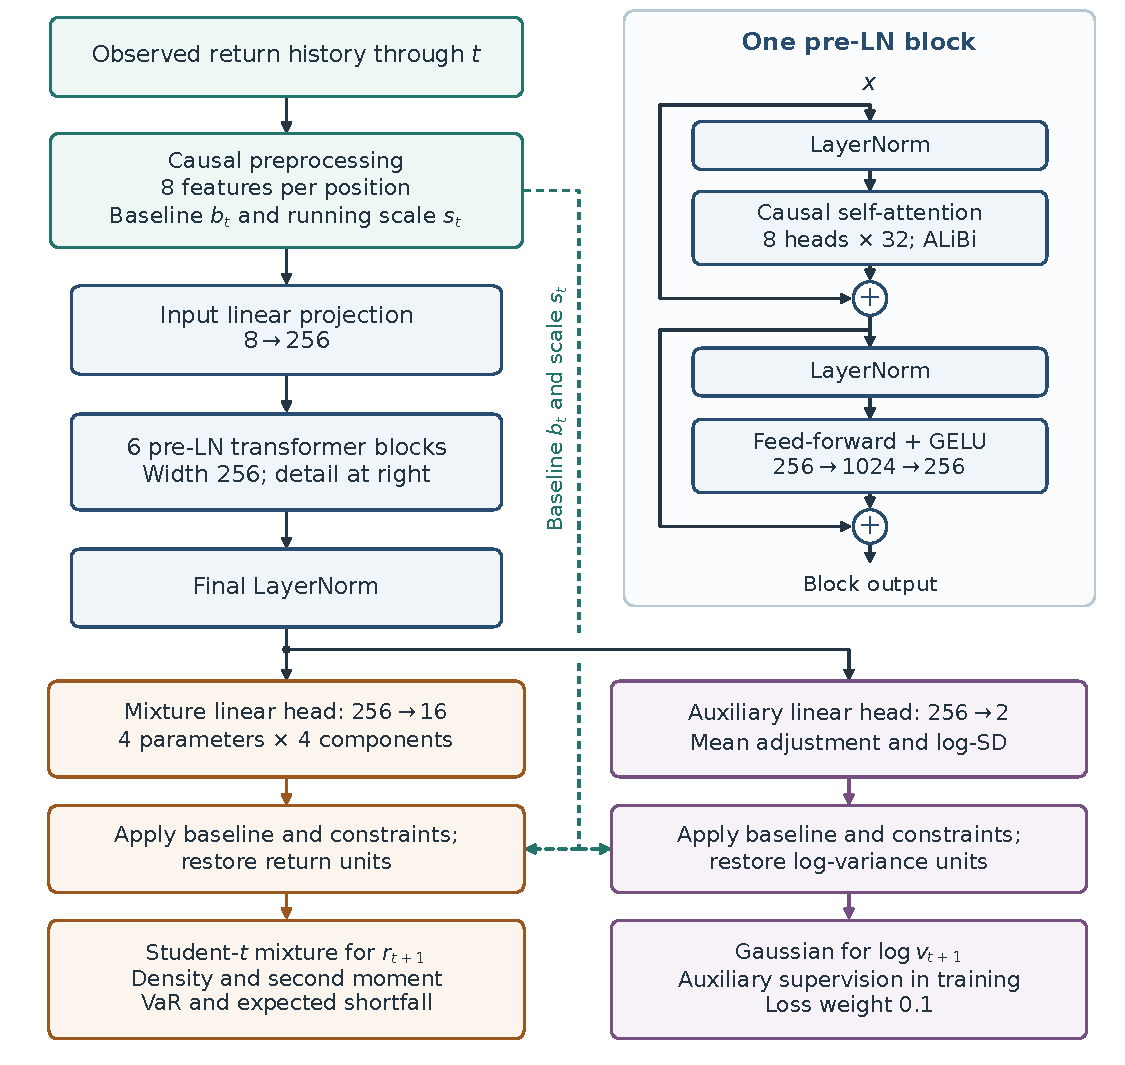
\includegraphics[width=\textwidth]{volpfn_architecture.pdf}
\caption[The implemented VolPFN architecture]{The architecture used by both prior arms. Each input position produces a distribution for the next return. The diagram is drawn from the verified implementation: self-attention and feed-forward components follow \citet{vaswani2017attention}, with pre-normalisation \citep{xiong2020layer} and an ALiBi-based distance bias \citep{press2022alibi}. The baseline uses an exponential average with a half-life of 20 nonzero observations and enters both output transformations. The auxiliary head supplies training supervision; the return forecast comes from the four-component mixture.}
\label{fig:volpfn-architecture}
\end{figure}

The input representation summarises the available history through eight channels: standardised return, magnitude, sign, zero status, three exponential risk estimates and position. Causal attention excludes future returns. The multiple risk horizons help distinguish a recent shock from a sustained change, following earlier volatility-modelling motivation without establishing each horizon as optimal \citep{corsi2009simple}. Appendix~\ref{app:forecast-details} specifies the transformations, layer sizes and distance-bias schedule \citep{vaswani2017attention,xiong2020layer,press2022alibi}.

To turn that representation into a return forecast, we combine four Student components. Their centres, scales and tail thicknesses can differ, giving more flexibility than one fixed Student law \citep{bishop1994mixture}. The issued density is

\begin{equation}
 q_t(x)=\sum_{k=1}^{4}w_{k,t}\,
 \frac{1}{s_{k,t}}f_{\nu_{k,t}}\!\left(\frac{x-\mu_{k,t}}{s_{k,t}}\right),
 \qquad \sum_k w_{k,t}=1.
 \label{eq:volpfn-density}
\end{equation}

The component law $f_\nu$ is the standard Student density; $w$, $\mu$, $s$ and $\nu$ denote weight, centre, scale and degrees of freedom. Weights are non-negative and sum to one, scales are positive, and degrees of freedom exceed two so that second moments exist. The network adjusts an exponential risk baseline that supplies the overall level. This baseline brings a running summary of past squared returns into the output transformation; the component parameters turn that baseline into a complete return distribution. From the mixture we obtain both the density and expected squared return, then subtract squared predictive mean when central variance is required.

Training connects these outputs to two objectives. The main return-density loss rewards probability assigned to observed returns. An auxiliary head predicts simulated log variance and its uncertainty through Gaussian negative log likelihood \citep{caruana1997multitask}, weighted 0.1. Its role is supervision, not the issued risk forecast, and both losses exclude stale targets. Chapter~\ref{ch:analysis} tests removal of the auxiliary objective and direct second-moment prediction. Chapter~\ref{ch:data} gives AdamW and the fixed allocation \citep{loshchilov2019decoupled}.

During market forecasting, new observations change the supplied history and its causal summaries, while the neural weights remain fixed. The forecast can therefore respond to market conditions without further neural training. Future-observation perturbations and input-window ownership checks confirm the causal implementation. We keep evidence from the retained earlier checkpoint separate because its normalisation differs from the corrected procedure.

\section{Corrected comparison with general pretrained forecasters}

\subsection{The comparison that the benchmark answers}

The first benchmark evaluates VolPFN alongside the specified Chronos-2, Moirai-2 and TabPFN-TS adapters \citep{ansari2025chronos2,liu2025moirai2,hoo2025tables}. All score the same 8,774 observations from 28 indices in April 2015--June 2016. Competitor forecasts stay fixed, while each of the five corrected VolPFN models fits a scale adjustment on the same development origins. We then evaluate fixed-calibration squared-return QLIKE with equal market weights and lower loss preferred.

This design ranks complete forecasting procedures. The systems differ in training data, representations and whether their output is a median or mean, so the result cannot isolate the prior's contribution. We address that narrower question through the controlled comparison in Section~\ref{sec:matched-prior}.

\subsection{Magnitude, uncertainty and consistency}

\begin{table}[!htbp]
\centering\small
\caption[Corrected five-model benchmark]{Corrected procedure: competitor minus VolPFN fixed-scale QLIKE. Positive gains favour VolPFN. Family-adjusted intervals and Holm-adjusted $p$-values concern the three primary comparisons with 10-date blocks. The sample is 8,774 market--date rows across 28 markets.}
\label{tab:corrected-benchmark}
\begin{tabular}{lrrrr}
\toprule
Comparator & Gain & Family 95\% interval & Holm $p$ & Markets \\
\midrule
Chronos-2 & 0.08083 & $[0.02265,0.15673]$ & 0.01220 & 26/28 \\
Moirai-2 & 0.07250 & $[0.02327,0.14085]$ & 0.01220 & 26/28 \\
TabPFN-TS & 0.14109 & $[0.07691,0.21846]$ & 0.00015 & 28/28 \\
\bottomrule
\end{tabular}
\end{table}

VolPFN leads the tested calibrated benchmark (Table~\ref{tab:corrected-benchmark}), with QLIKE gains of about 0.081, 0.073 and 0.141 over Chronos-2, Moirai-2 and TabPFN-TS respectively. Every seed improves on every comparator, and all three family intervals are positive. These gains are absolute loss differences rather than accuracy percentages. Market breakdowns retain the exceptions: Chronos-2 and Moirai-2 each win on two markets, while VolPFN improves on TabPFN-TS in all 28. This performance claim is limited to the specified calibrated alternatives.

\begin{figure}[!htbp]
\centering
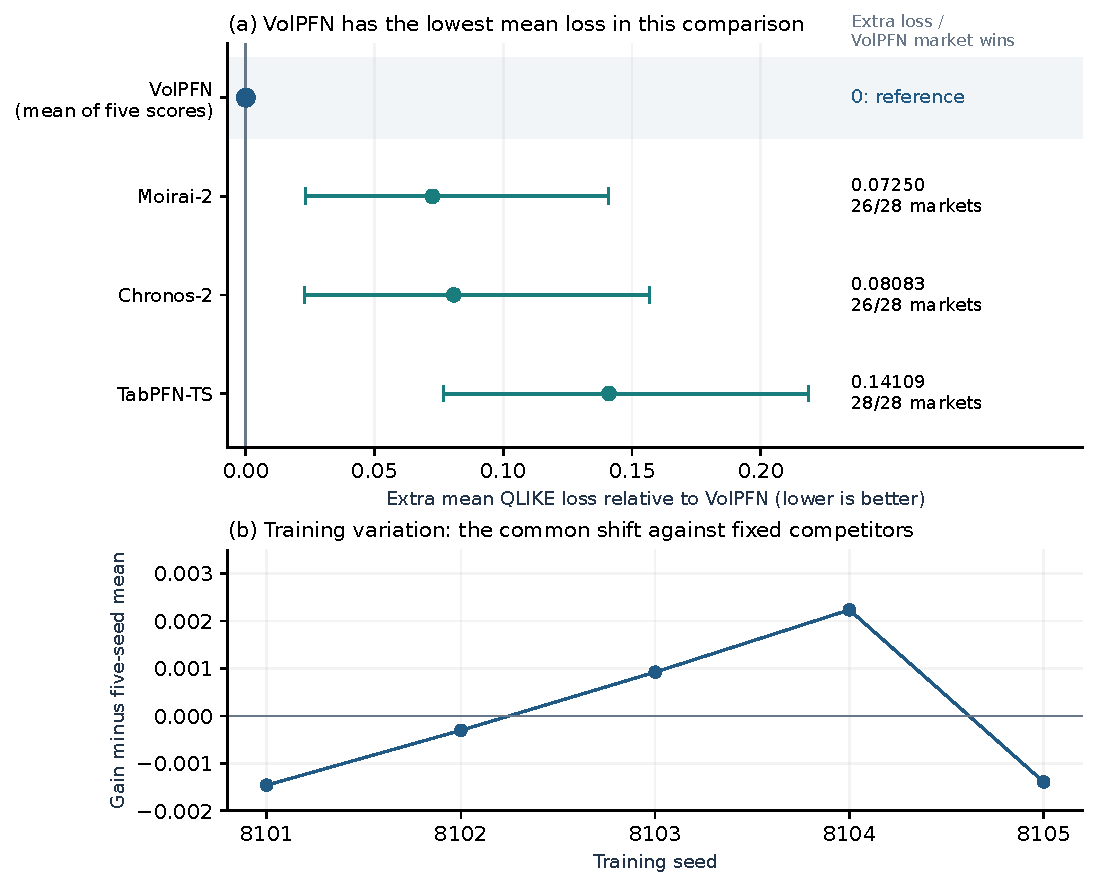
\includegraphics[width=\textwidth]{forecasting_benchmark_rank.pdf}
\caption[VolPFN leads the tested benchmark comparison]{Fixed-scale QLIKE on 8,774 rows across 28 markets, April 2015--June 2016. Top: competitors' excess loss relative to the mean score of five VolPFN models, with family-adjusted 95\% calendar-block intervals and market wins. VolPFN's zero is a reference, not an estimate with zero uncertainty. Bottom: each seed's gain minus the five-model mean; this shift is common across fixed competitors. Scores are averaged across models, not ensemble predictions. The recorded adapters, fitted development scales and historical exposure define the comparison.}
\label{fig:corrected-benchmark}
\end{figure}

All three conclusions survive the alternative calendar-block lengths. Figure~\ref{fig:corrected-benchmark} also shows that similar mean scores across seeds can coexist with appreciable uncertainty across dates. Appendix~\ref{sec:supplementary-forecasting} retains the complete seed and market breakdowns. The supported claim remains performance of these calibrated pipelines on this panel.

\FloatBarrier

\section{Financial benchmarks and realised-risk information}

We next broaden the competitor set and the information supplied to forecasts. Because these studies use different periods and separately adjusted families, each result needs to be interpreted within its own comparison. Table~\ref{tab:study_map} records those boundaries.

\subsection{Dedicated daily financial predictors}
\label{sec:new-daily-comparison}

The completed ARCH-LSTM, GARCH-LSTM and GINN adaptations provide dedicated daily financial comparisons on 28 markets in 2015--February 2022. We compare their squared-return QLIKE with full VolPFN on the retained observations, reporting each competitor's loss minus full's loss. Full improves over all three, with gains of about 0.046--0.376 (Table~\ref{tab:new-daily-gains}). All five seed means and all 28 market means favour it, and block-length sensitivities retain the adjusted conclusions. Full is the pre-specified reference, selected before inspecting these comparison outcomes.

\begin{table}[!htbp]\centering
\begingroup\small\setlength{\tabcolsep}{4pt}
\caption[Gains against daily financial neural predictors]{Full VolPFN versus the dedicated daily adaptations, 2015--February 2022. The four-slot external family retains unavailable RECH at $p=1$. Ordinary 95\% intervals are not simultaneous intervals. Gains favour full when positive.}\label{tab:new-daily-gains}
\begin{tabular}{@{}>{\raggedright\arraybackslash}p{4.1cm}rcr@{}}
\toprule
Comparison & Gain & Ordinary 95\% interval & Holm $p$ \\
\midrule
ARCH-LSTM & 0.376213 & $[0.295777,0.453705]$ & 0.000200 \\
GARCH-LSTM & 0.070375 & $[0.050145,0.089188]$ & 0.000200 \\
GINN & 0.046427 & $[0.031970,0.059823]$ & 0.000200 \\
rech & --- & --- & 1.000000 \\
\bottomrule
\end{tabular}\endgroup\end{table}


The financial predictors fit each market separately and have different contexts and validation choices, whereas VolPFN learns from simulation. The comparison therefore concerns these completed adaptations without isolating architecture or reproducing every published setting. Appendix~\ref{sec:new-research-results} retains the failed historical configuration and unavailable RECH comparison alongside the successful procedures.

\subsection{A harmonised daily-return panel}
\label{sec:new-harmonised-daily}

To assess the wider daily leaderboard on common observations, we align saved raw forecasts on 22,026 market--date keys in 2019--February 2022. VolPFN variants lead the evaluated daily-return-only procedures at both squared-return and realised-kernel QLIKE. The set includes conventional volatility models, dedicated financial networks and general pretrained forecasters such as TabPFN-TS. Full scores about 0.704 and 0.626. The complete two-target rule for full supports improvement over ARCH-LSTM, Chronos-2, GARCH-LSTM, TabPFN-TS and UniVol, but not over GJR-GARCH despite a lower mean. Observed leadership consequently does not establish superiority over every competitor.

Noaux and the earlier VolPFN version have slightly lower means than full, but their descriptive ranks do not inherit its tests. The complete leaderboard retains Moirai's floor-associated losses and EGARCH's extreme forecasts as outcomes of the issued procedures (Appendix~\ref{sec:new-research-results}). The independently fitted compact rule remains a separate historical alternative. TTM's lower diagnostic scores involve intraday information and belong to a different information comparison.

\subsection{Adding realised-risk forecasts}
\label{sec:new-intraday-comparison}

We then add intraday information without retraining the daily network by combining its forecast with Tiny Time Mixers (TTM), which uses past realised kernels. We call this additional predictor a \emph{helper}. For market $m$, date $t$, risk target $p$ and seed $s$, the combination is

\begin{equation}
 \log h_{m,t}^{p,s}=a_t^{p,s}+w_t^{p,s}\log h_{A,m,t}^{p,s}
 +(1-w_t^{p,s})\log h_{B,m,t}^{p,s}.
 \label{eq:new-online-blend}
\end{equation}

Here $A$ is the daily predictor and $B$ is the helper. We fit the intercept $a$ and weight $w$ using earlier completed observations pooled across markets. The intercept adjusts the overall level, while the weight changes the relative contributions and may fall outside $[0,1]$ because it is unconstrained. During the first sixty union dates, we use $a=0$ and $w=0.5$, then update every twenty union dates; a union date occurs in at least one included market. Squared-return fitting uses second moment, whereas realised-kernel fitting uses central variance. Since the two targets are fitted separately, their combinations do not define a single return density.

VolPFN+TTM scores about 0.672 and 0.599 at the two targets, while GNNHAR retains lower descriptive means of about 0.669 and 0.595 (Figure~\ref{fig:new-intraday}). The joint rule supports the combination over standalone full VolPFN, the 26 September version and GJR-GARCH. Comparisons with GNNHAR, QLIKE-HAR, Transfer-XGBoost, raw TTM and GJR+TTM remain unresolved. Passing an adjusted test alone is insufficient when its family interval crosses zero; both requirements must hold.

\begin{figure}[!htbp]\centering
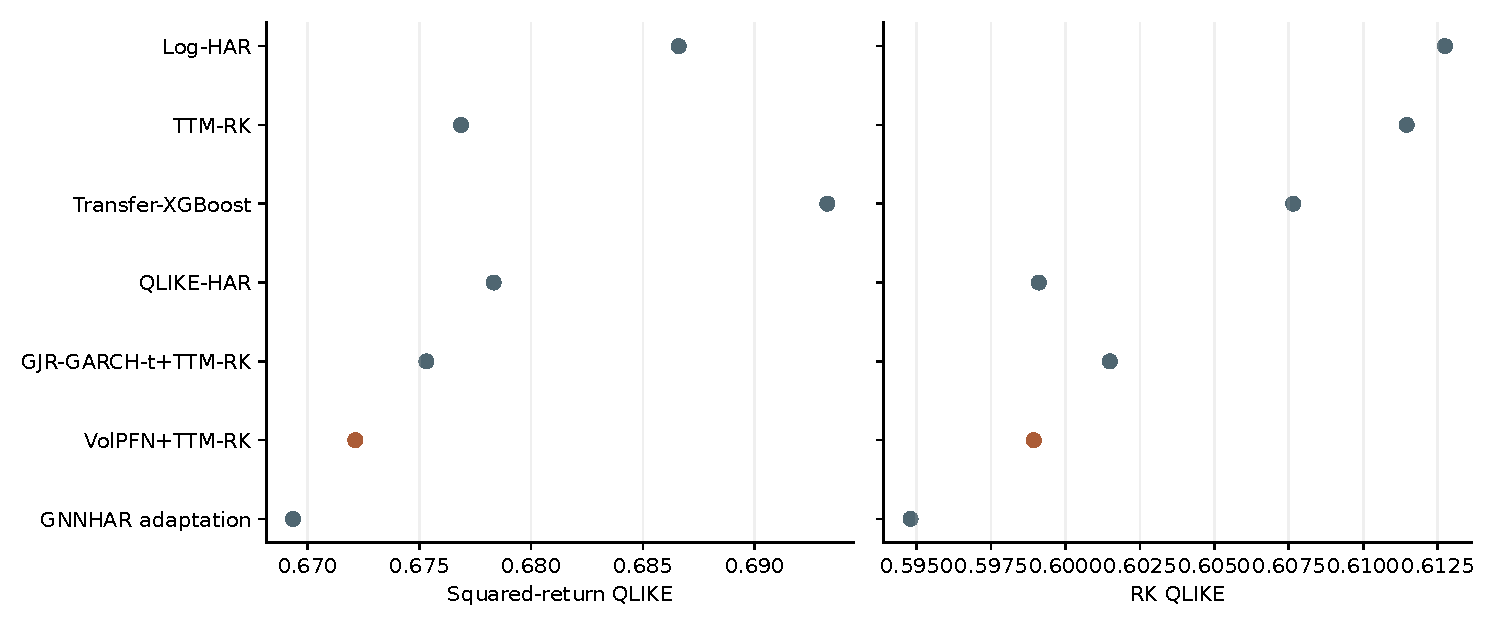
\includegraphics[width=\textwidth]{new_intraday_comparison.pdf}
\caption[Selected realised-risk procedures on common keys]{Descriptive QLIKE for selected complete procedures on the same 2019--February 2022 keys. Both proxy scores retain GNNHAR's lower mean. These points have no significance labels; information access and fitting opportunities differ, and the complete 38-slot rule determines supported comparisons.}
\label{fig:new-intraday}
\end{figure}

The blend changes both the information entering the forecast and the way its level is fitted. To examine the latter explanation, the October follow-up tests whether calibrating TTM alone recovers the combination's advantage on the same 22,026 observations. Its primary control fits $\log h=a+b\log h_{\mathrm{TTM}}$, giving two parameters to adjust level and response, as in the blend. A secondary control fits only a multiplicative scale. Both issue raw TTM during the first sixty union dates, then refit every twenty dates on strictly earlier completed observations pooled across markets. Risk targets are fitted separately. The affine control retains the blend's optimiser and tolerances, and the recorded follow-up replay reproduces its calculation to floating-point precision.

\begin{table}[!htbp]\centering\small
\caption[TTM-only causal calibration controls]{Saved blend and completed TTM-only controls on the same 22,026 keys, 28 markets, 2019--February 2022. Lower QLIKE is better. Raw TTM and GJR+TTM are descriptive here; the four-slot family compares the VolPFN blend with the two calibration controls at both proxies.}
\label{tab:followup-ttm}
\begin{tabular}{lrr}
\toprule
Procedure & Return QLIKE & RK QLIKE \\
\midrule
VolPFN+TTM blend & 0.672139 & 0.598944 \\
GJR+TTM blend & 0.675318 & 0.601493 \\
Saved standalone TTM & 0.676869 & 0.611457 \\
Scale-calibrated TTM & 0.681754 & 0.612566 \\
Affine-calibrated TTM & 0.685450 & 0.622200 \\
\bottomrule\end{tabular}
\end{table}


Control loss minus combination loss measures the gain beyond TTM-only calibration. The affine gains are about 0.013 for squared returns and 0.023 for RK, with adjusted $p=0.002$ and $p=0.004$. Scale-only gains are about 0.010 and 0.014, with adjusted $p=0.004$ and $p<0.001$. Every reference seed improves and all four family intervals are positive; twenty- and 120-date sensitivities retain support (Appendix~\ref{sec:followup-results}). TTM-only calibration worsens its mean score on the saved panel, and a descriptive check excluding the initial period retains the ordering.

The follow-up establishes predictive value beyond those specified calibration controls, without identifying daily information as the unique cause. Warm-up forecasts differ between the controls and blend. Raw TTM and GJR+TTM comparisons remain unresolved, and GNNHAR still has lower descriptive losses. Foreign histories and pooled fitting further restrict attribution to the daily predictor alone. RK publication vintages are also unverified: placing a measurement before the target session does not by itself show that this version of the measurement was available then.

A supplementary XGBoost helper draws 84 features from the target and other markets. All 140 fitted models issued forecasts, and its blend scores about 0.674 and 0.604. However, no contrast passes the separate twelve-comparison joint rule. We have not removed foreign-market inputs with other settings fixed, so their presence does not establish a causal benefit. Appendix~\ref{sec:new-research-results} retains the controls and complete losses.

Additional realised-risk information improves some completed procedures, but the comparisons do not establish this blend as the best realised-risk forecast. This limits the performance claim and separates it from the question of what the standalone daily prior contributes.
\FloatBarrier

\section{Frozen evaluation on a new ETF population}
\label{sec:external-etfs}

The ETF study extends the asset population to test transfer beyond stock-market indices. Original full/noaux weights and the historical model selected on earlier index development data score the same 22,600 session returns from twenty ETFs in March 2022--August 2026. ETF outcomes neither select checkpoints nor update neural weights. Rolling GJR follows the frozen causal fitting policy in Chapter~\ref{ch:data}.

\begin{table}[!htbp]\centering\small
\caption[Frozen external ETF scores]{Frozen twenty-ETF population, 22,600 rows per model/seed, March 2022--August 2026. Means weight ETFs and neural seeds equally. Squared-return QLIKE is primary; native NLL is descriptive. Lower is better. Original full/noaux weights and index-development-selected historical weights receive no ETF training.}
\label{tab:followup-etfs}
\begin{tabular}{lrr}
\toprule
Procedure & Return QLIKE & Native NLL \\
\midrule
Synthetic noaux & 0.437251 & 1.111585 \\
Synthetic full & 0.438591 & 1.111583 \\
Rolling GJR-GARCH-$t$ & 0.452051 & 1.117771 \\
Development-selected historical & 0.458122 & 1.138492 \\
\bottomrule\end{tabular}
\end{table}


On matched ETF observations, noaux improves on the historical procedure by about 0.021 QLIKE units, with Holm-adjusted $p=0.03$ and a positive family interval. All five seed gains and eighteen of twenty ETF means favour noaux, and both alternative block lengths retain support. Full and noaux have lower means than rolling GJR by about 0.013 and 0.015, but adjusted $p$-values near 0.10 and family intervals crossing zero leave superiority unresolved (Appendix~\ref{sec:followup-results}). Native density losses remain descriptive rather than an additional superiority endpoint.

This supports the synthetic procedure over the improved historical comparator on the fixed external population. It does not repeat broad--Mat\'ern matching: training source, regularisation and checkpoint selection differ. The protocol predates acquisition, while human exposure remains unverified and the dates share index-study shocks. We therefore interpret this as external population validation subject to those qualifications. The following density results use an earlier checkpoint and another fitting schedule, so their margins stay separate.
\FloatBarrier

\section{Historical density comparisons}
\label{sec:historical-density}

The retained earlier checkpoint allows us to evaluate complete return distributions alongside risk forecasts. It differs from the corrected five-model set and uses repaired causal inference on 28 indices: 26,293 development observations in 2011--2014 and 50,073 later observations in 2015--February 2022. These results complement, rather than replace, the corrected comparisons.

We compare its densities with rolling GARCH-$t$, UniVol and EWMA$(0.94)$ with $t_8$ tails \citep{bollerslev1986generalized,riskmetrics1996}. GARCH fits 1,000 preceding returns every 250 observations. UniVol combines score-driven filters and restart experts, updating their weights through log score. Appendix~\ref{sec:supplementary-forecasting} preserves the schedules and expert grid.

\subsection{What native and common-law scores reveal}

Native scoring evaluates each complete issued distribution, allowing both its scale and shape to affect the result. Common-$t_8$ scoring instead compares scale under one Student law: GARCH supplies variance with fitted mean suppressed, while VolPFN and UniVol supply second moments. UniVol uses its mixture's arithmetic moment rather than its geometric point forecast. All three forecasts are scored under the common law, while the other procedural differences remain.

\begin{table}[!htbp]
\centering
\caption[Development density comparisons]{Development log-density differences, 2011--2014. Positive values favour VolPFN. Intervals are conditional circular observed-date bootstrap intervals.}
\label{tab:development-density}
\small
\begin{tabular}{llrrr}
\toprule
Comparator & Distribution & Difference & 95\% interval & Markets \\
\midrule
GARCH-$t$ & Native & $+0.01714$ & $[0.01352,0.02102]$ & 28/28 \\
UniVol & Native & $+0.01211$ & $[0.00751,0.01662]$ & 27/28 \\
GARCH & Common $t_8$ & $+0.01327$ & $[0.00951,0.01739]$ & 26/28 \\
UniVol & Common $t_8$ & $+0.01025$ & $[0.00665,0.01385]$ & 27/28 \\
\bottomrule
\end{tabular}
\end{table}

Positive development gains under the common law show that flexible shape cannot account for the whole native-density advantage (Table~\ref{tab:development-density}). Subtracting the two margins would not isolate shape because both forecasts change. We instead exchange saved scales and standardised shapes in both replacement orders and average their contributions. The substitution assigns about 0.0078 nats to scale and 0.0043 to shape (Table~\ref{tab:clarity-precision}), with shape including centres, asymmetry and mixture structure. It describes differences between issued forecasts rather than causes in training.

\begin{figure}[!htbp]
\centering
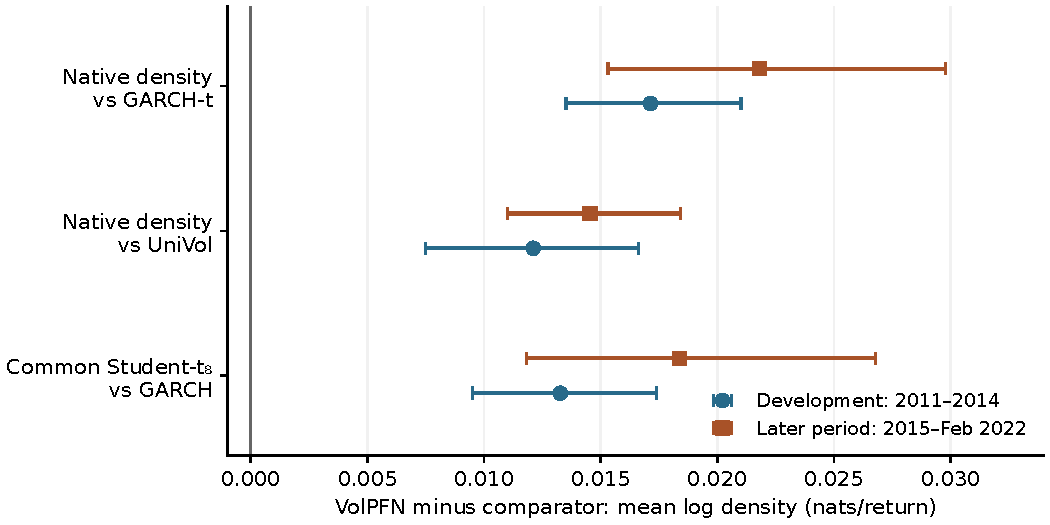
\includegraphics[width=\textwidth]{density_comparison_new.pdf}
\caption[Density gains in two evaluation periods]{Retained-checkpoint equal-market log-density differences on 28 indices. Bars show 95\% circular observed-date bootstrap intervals, conditional on the retained forecasts. Positive values favour VolPFN. They exclude training and model-selection uncertainty; the later period has the prior exposure described in the text.}
\label{fig:density-new}
\end{figure}

The historical later-period rule requires a positive panel mean, bootstrap tail area below 0.05 and gains in at least twenty of 28 markets. We measure calendar uncertainty through 2,000 circular resamples of sixty observed union dates, moving markets together to retain shared shocks. This rule is distinct from the corrected benchmark's multiplicity adjustment.

\begin{table}[!htbp]
\centering
\caption[Later-period density comparisons]{Later-period density comparison, 2015--February 2022. Differences are in nats per return and give equal weight to each of 28 markets.}
\label{tab:confirmation-density}
\small
\begin{tabular}{llrrr}
\toprule
Comparator & Distribution & Difference & 95\% interval & Markets \\
\midrule
GARCH-$t$ & Native & $+0.02181$ & $[0.01532,0.02977]$ & 28/28 \\
UniVol & Native & $+0.01454$ & $[0.01102,0.01841]$ & 28/28 \\
EWMA$(0.94)$--$t_8$ & Native & $+0.02453$ & $[0.01833,0.03169]$ & 28/28 \\
GARCH & Common $t_8$ & $+0.01838$ & $[0.01182,0.02677]$ & 28/28 \\
\bottomrule
\end{tabular}
\end{table}

All four retained later-period comparisons satisfy the historical rule and favour VolPFN in all 28 markets (Table~\ref{tab:confirmation-density}). Native gains are about 0.015--0.025 nats per return, and the common-law GARCH gain is positive. Archived two-sided tail areas reach the resampling floor. These comparisons meet the historical decision rule; they are outside the corrected benchmark family.

The intervals describe date variation conditional on retained forecasts. Prior contact with the pipeline and tail data, documented in Section~\ref{sec:exposure}, restricts their interpretation as independent confirmation.

Market and yearly breakdowns show variation in the margin without identifying one shared crisis mechanism (Appendix~\ref{sec:supplementary-forecasting}). Appendix~\ref{app:alternative-checks} retains the supporting density-average and finite-prior comparisons.

VolPFN's lead in the tested general benchmark and its variants' lead in the daily-return-only leaderboard leave two questions open: how much the prior contributes and how much performance a simpler rule can retain. The next chapter examines both by matching neural training settings and fitting compact rules. Superiority over the stronger realised-risk alternatives remains unresolved.

\chapter{Prior contribution and limits of the explanation}
\label{ch:analysis}

The forecasting comparisons establish where VolPFN is useful, but leave the explanation of its advantage open. We investigate that explanation in stages: matching two simulation designs, changing training loss and output, and strengthening the historical comparator. We then ask whether a small rule retains useful prediction and whether the network tracks simulated volatility nearly as well as a privileged reference. Each comparison tests a different part of the proposed explanation.

\section{A matched test of the prior package}
\label{sec:matched-prior}

To test the prior's contribution, we train network pairs on different simulated histories while matching the remaining settings. Matching initial weights and training allocation reduces variation from initialisation, duration and checkpoint selection. The intended intervention is the simulation design, which allows a more specific interpretation than a comparison between unrelated forecasting systems.

\subsection{Why this alternative, and what changes?}

The broad design samples seven volatility families (Table~\ref{tab:simulation-prior}). Its Mat\'ern alternative draws a hidden log-variance path from a Gaussian-process covariance model \citep{rasmussen2006gaussian}, varying irregularity and persistence without a return-driven scale recursion. Applied to the turbulent-week illustration, these designs provide different explanations of similar observed returns.

For Mat\'ern histories, we sample equally from nine combinations of smoothness values 0.1, 0.5 and 1.5 and length scales 30, 120 and 500 observations. Log-variance standard deviation is uniform between 0.3 and 1.5. These are specified settings rather than literature-prescribed optima. Both experimental \emph{arms} retain the same innovation generator and probabilities of jumps, serial correlation, drift and stale observations. The comparison changes latent-volatility design while sharing these disturbances. Overlapping diagnostic ranges do not make all observable features identically distributed, and this construction represents one alternative rather than every generic prior.

All five pairs retain the \emph{fixed-final} checkpoint at update 20,000 without validation-based selection. Architecture, normalisation, losses, optimisation and allocation agree within pairs, although their random histories may differ. The intervention therefore concerns the combined design under a finite recorded training procedure, not an idealised fully converged predictor (Appendix~\ref{app:closure_protocol}).

\subsection{The target and decision rule}

Acquisition and quality gates define the population before scoring. Both models then forecast the same roughly 22,500 returns across twenty indices in March 2022--August 2026. Eight candidates fail the rules rather than being excluded because of forecast gains. Prior contact with these histories remains documented in Section~\ref{sec:exposure}.

We compare scale by converting each predicted second moment to the zero-centred Student law with eight degrees of freedom defined in Chapter~\ref{ch:data}. The common-$t_8$ law holds scoring tails fixed, while the mixture output still affects the second moment being converted. No fitted multiplier can absorb differences in forecast level. We average scores across dates within markets, then give markets and seeds equal weight, so longer histories do not receive greater panel weight.

The decision rule considers uncertainty, the chosen effect-size threshold and market breadth. Section~\ref{sec:inference} specifies the tests, a mean of at least 0.005 nats per return and positive means in at least fifteen markets. The reserved broad-versus-GARCH slot stays in the multiplicity family despite being unrun. Equivalence uses its separate $\pm0.003$-nat margin. These requirements are unchanged from the specified decision rule.

\subsection{Results and their magnitude}

\begin{table}[!htbp]
\centering\small
\caption[Five matched prior pairs]{Broad-minus-Mat\'ern common-$t_8$ log-score gain, in nats per return. Each row pairs models with matching initialisation and training settings. All rows use the same locked 20-market sample.}
\label{tab:matched-prior-seeds}
\begin{tabular}{lr}
\toprule
Seed pair & Gain \\
\midrule
8101 & 0.005942 \\
8102 & 0.005217 \\
8103 & 0.004745 \\
8104 & 0.004335 \\
8105 & 0.005661 \\
\midrule
Equal-seed mean & 0.005180 \\
95\% conditional interval & $[0.001862,0.008151]$ \\
Holm-adjusted $p$ & 0.003199 \\
Positive markets & 17/20 \\
\bottomrule
\end{tabular}
\end{table}

The broad-minus-Mat\'ern common-$t_8$ gain averages about 0.0052 nats per return (Table~\ref{tab:matched-prior-seeds}). All five paired means and seventeen of twenty market means are positive. The conditional interval excludes zero, the adjusted test passes and the mean clears the size threshold. The experiment therefore meets all three requirements: support, magnitude and breadth.

Exponentiating the mean difference gives roughly half a percent higher density at observed returns on a geometric-average basis. This is a modest forecasting improvement rather than an investment return. The aggregate only narrowly clears 0.005, two pair means fall below that threshold, and a positive interval does not show that the population gain exceeds it. The equivalence interval also falls outside the declared band; Appendix~\ref{sec:prior-interpretation-details} retains its exact endpoints.

\begin{figure}[!htbp]
\centering
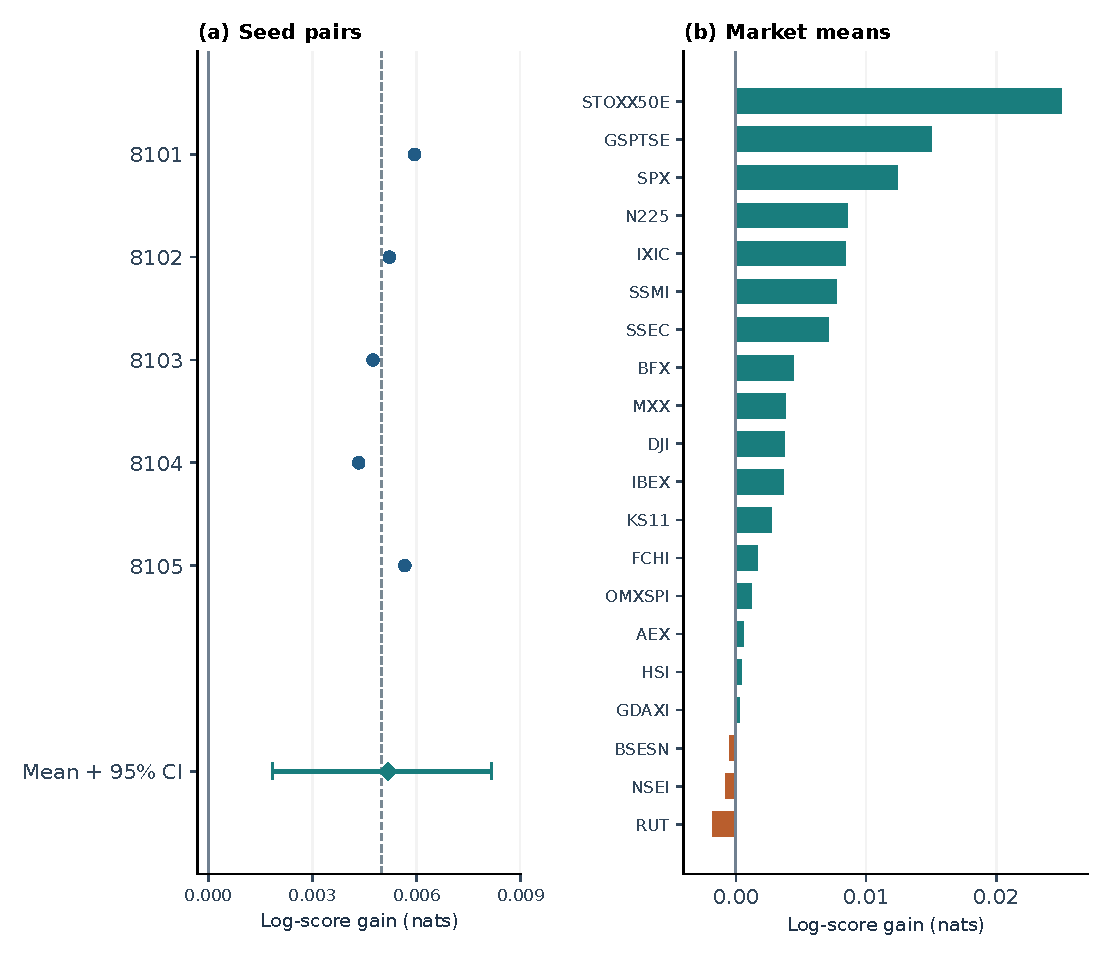
\includegraphics[width=\textwidth]{matched_prior.pdf}
\caption[Prior substitution by seed and market]{The broad-minus-Mat\'ern common-$t_8$ gain. Left: all five paired means and the aggregate conditional 95\% interval; the dashed line is the point-materiality gate, not a confidence bound. Right: the twenty equal-seed market means, with three negative values retained. Market and seed dots are descriptive, not separately tested effects.}
\label{fig:matched-prior}
\end{figure}

We next assess how concentrated the aggregate gain is by omitting market summaries from descriptive averages. STOXX50E, GSPTSE and SPX contribute about half of the net gain (Figure~\ref{fig:matched-prior}), so we examine their individual and joint omissions. These post-result calculations neither redefine the registered population nor create another confirmatory test.

\begin{figure}[!htbp]
\centering
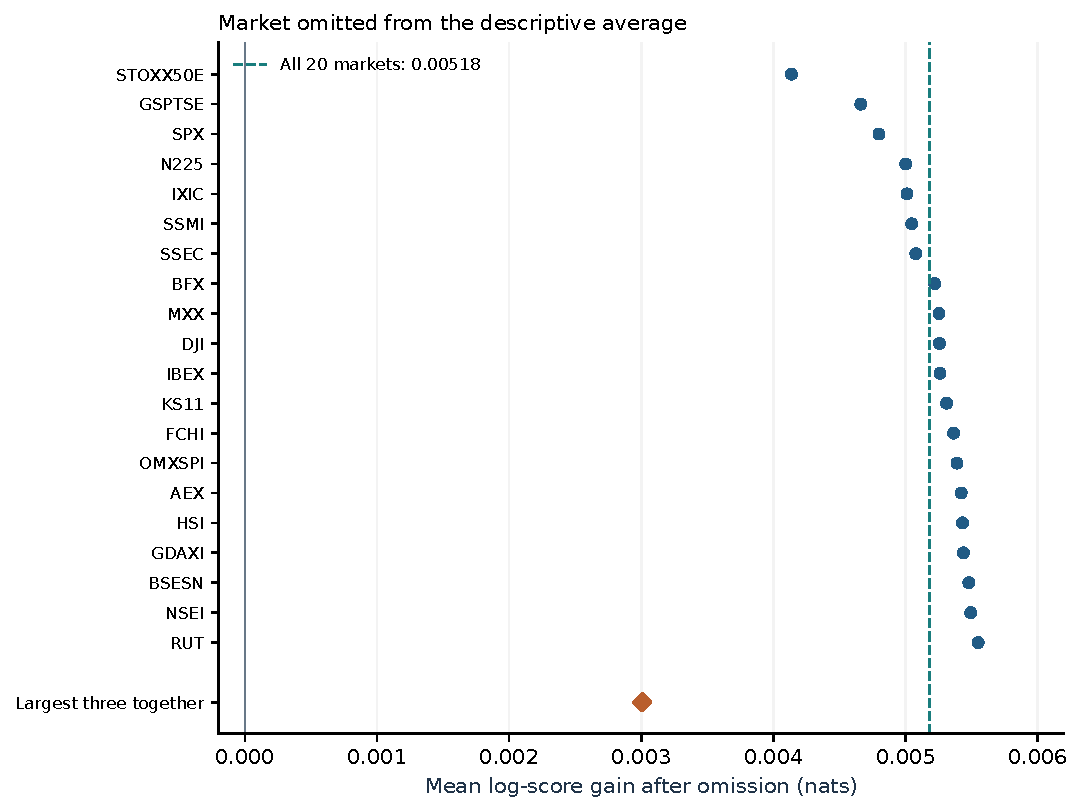
\includegraphics[width=\textwidth]{prior_market_influence.pdf}
\caption[Descriptive influence of individual markets]{Sensitivity of the broad-minus-Mat\'ern mean gain to omitting market summaries. Each single-omission point averages the remaining nineteen markets. The separate three-market omission excludes STOXX50E, GSPTSE and SPX, the largest observed positive contributors. These are post-result descriptive calculations on existing scores, with no new confidence intervals or registered hypothesis tests. The original twenty-market decision is unchanged.}
\label{fig:prior-market-influence}
\end{figure}

Every single-market omission leaves a positive mean of roughly 0.004--0.006 nats per return. Removing the three largest contributors together leaves about 0.003 across seventeen markets (Figure~\ref{fig:prior-market-influence}). The direction does not depend on one market, although the size depends on panel composition. Without additional intervals, these descriptive summaries establish no separate population effect.

The result supports the combined simulation design relative to this Mat\'ern alternative. Because several properties change together, it does not isolate return feedback, asymmetry or regime switching as the cause. Uncertainty also conditions on the ten fitted networks. A narrower matched intervention would be needed to identify one mechanism. We now turn to the completed changes in supervision, output and training source.

\section{What the component interventions establish}
\label{sec:new-components}

The component programme retains the supplied update budget while changing stated configurations. Its twenty runs compare auxiliary volatility supervision, distribution versus direct risk prediction, and synthetic versus historical windows on the 2015--February 2022 panel (Table~\ref{tab:new-components}). The results apply to these tested configurations rather than every implementation of each component.

\begin{table}[!htbp]\centering
\begingroup\small\setlength{\tabcolsep}{4pt}
\caption[Matched training-component interventions]{Component interventions, 2015--February 2022. Gain is comparator minus named reference squared-return QLIKE; positive favours the reference. All five seeds and 28 markets remain. Ordinary intervals and Holm probabilities use the separate three-slot family, 20,000 draws and 60-date blocks.}\label{tab:new-components}
\begin{tabular}{@{}>{\raggedright\arraybackslash}p{4.1cm}rcr@{}}
\toprule
Comparison & Gain & Ordinary 95\% interval & Holm $p$ \\
\midrule
Full versus noaux & -0.000581 & $[-0.001499,0.000321]$ & 0.206540 \\
Density noaux versus direct & 0.009540 & $[0.004052,0.015214]$ & 0.001300 \\
Synthetic versus historical noaux & 220.701975 & $[168.500456,263.777505]$ & 0.000150 \\
\bottomrule
\end{tabular}\endgroup\end{table}


Removing the simulated-volatility loss produces \emph{noaux}, while \emph{full} retains it. We detect no deterioration from removal: full's estimated gain is slightly negative and its interval crosses zero. Two seeds favour full and three favour noaux. Keeping the unused noaux head preserves initialisation matching. Its continued presence does not supply volatility supervision because that loss has been removed. This result concerns the tested supervision weight and budget; it establishes neither equivalence nor the absence of a useful alternative setting.

The noaux distribution configuration improves QLIKE over direct expected-squared-return prediction by about 0.010, with a positive interval and passing adjusted test. Matching the initial trunk and supplied synthetic batches controls those settings, but output and loss still change together. The evidence therefore supports the combination of output and loss. Direct has no native return distribution, and conversion to common-$t_8$ scoring does not create a learned density.

\begin{figure}[!htbp]\centering
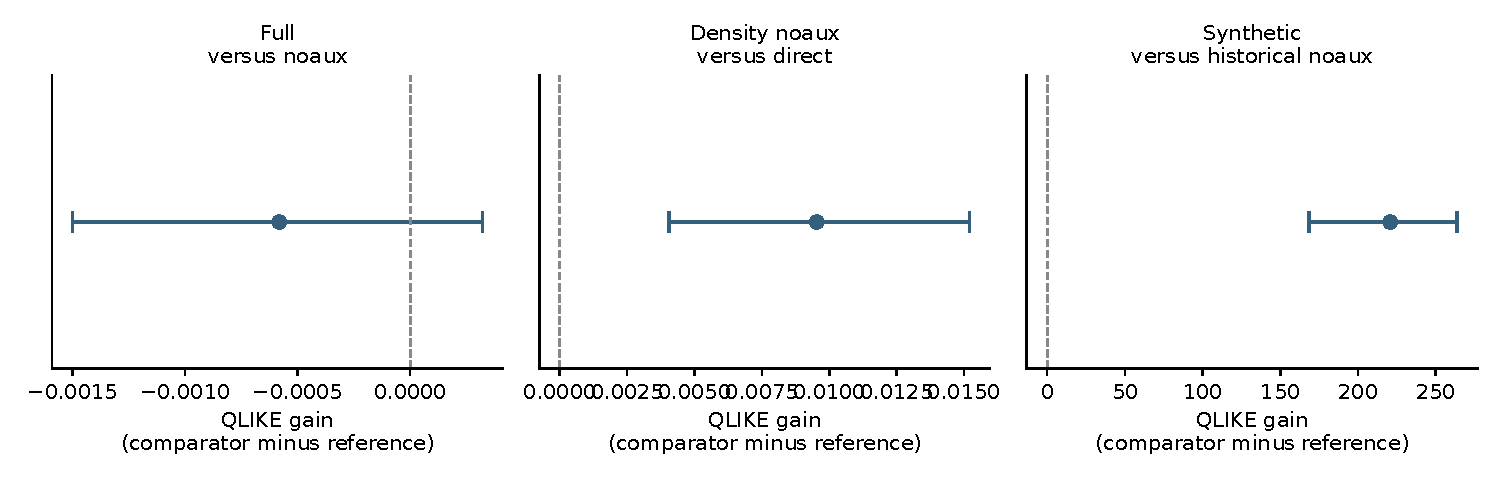
\includegraphics[width=\textwidth]{new_component_gains.pdf}
\caption[The three component interventions]{Comparator-minus-reference QLIKE gains and ordinary conditional 95\% intervals for the three registered component comparisons. Each panel has its own numerical axis because the historical failure is much larger. The intervals are not simultaneous; the separate three-slot Holm family supplies the adjusted tests.}
\label{fig:new-components}
\end{figure}

The original fixed-final historical model severely underpredicts some later risks. Mean QLIKE is about 221 versus 0.59 for synthetic noaux, despite a historical median near 0.55. More than fifteen thousand seed-level forecasts exceed QLIKE 100. This difference between mean and median shows why a typical-observation summary would hide the failures. Appendix~\ref{sec:prior-interpretation-details} retains exact counts.

The recorded checks of targets, scaling, alignment and the evaluation path found no clear defect. Historical training repeats about 70,000 distinct observations; low late-training likelihood loss alongside poor later calibration is consistent with memorisation or density collapse. These diagnostics do not identify a sole cause. The failure concerns that optimisation and selection procedure; it does not establish general inferiority of historical training. To assess how much the source comparison depends on this failure, the follow-up changes regularisation and allows development data to select an earlier checkpoint.

\subsection{What development-selected historical training changes}
\label{sec:improved-historical}

The October historical follow-up adds residual dropout and selects weights on earlier index development observations. Its five seeds use the original return mask and attain mean QLIKE near 0.60, compared with synthetic means near 0.59 (Table~\ref{tab:followup-historical}). All five runs selected update 500 and stopped at 3,500. Each run retains one QLIKE-above-100 event; the original five runs together had more than fifteen thousand. No difficult observation is removed.

\begin{table}[!htbp]\centering\small
\caption[Stronger historical comparator]{Equal-market/seed squared-return QLIKE on the unchanged 50,073 index rows per seed, 2015--25 February 2022. Lower is better. The original failed procedure is preserved separately as an optimisation diagnostic; inferential contrasts use the development-selected historical procedure.}
\label{tab:followup-historical}
\begin{tabular}{lr}
\toprule
Procedure & QLIKE \\
\midrule
Synthetic noaux & 0.590118 \\
Synthetic full & 0.590700 \\
Development-selected historical & 0.602085 \\
Original historical (diagnostic) & 221.292094 \\
\bottomrule\end{tabular}
\end{table}


Subtracting synthetic loss from historical loss gives an estimated synthetic advantage of about 0.012 QLIKE units for noaux and 0.011 for full. Every paired-seed gain is positive. However, support also requires the adjusted test and family interval to pass: both family intervals cross zero and adjusted probabilities are about $p=0.08$, even though noaux's ordinary interval is positive. Neither contrast therefore meets the complete rule. Twenty- and 120-date sensitivities retain this conclusion, while native and common-law density losses remain descriptive (Appendix~\ref{sec:followup-results}). The estimated lead is modest, and the family-level evidence is insufficient to establish superiority.

Historical training is therefore competitive under the stronger procedure, narrowing the training-source interpretation of the original failure. Synthetic models retain a modest estimated index lead, and the ETF study supports noaux over the improved historical procedure (Section~\ref{sec:external-etfs}). Dropout, checkpoint selection and selected duration also differ, so these comparisons do not isolate training source or architecture alone.

The component evidence supports the tested distribution output and loss, while the historical follow-up restricts the source claim. Neither decomposes the matched-prior gain or benchmark margins. Figure~\ref{fig:followup-primary} and Appendix~\ref{sec:followup-results} bring the three follow-up families together without pooling populations or multiplicity rules. The compact and tail studies retain their original checkpoint. We next ask how much of that checkpoint's forecasting advantage a small independent rule can retain.

\FloatBarrier

\section{How much forecasting needs a neural model?}
\label{sec:compact-rule}

The compact studies fit an explicit updating formula that subsequently forecasts without the network. They use the retained earlier checkpoint and development panel. Score-driven models motivate interpretable updating \citep{creal2013generalized,harvey2013dynamic}, although our fitted formula is not a bounded score-driven update. We test retained forecasting advantage rather than reproduction of a known neural algorithm.

We compare three nested rules to assess how the added terms affect attained forecasting performance. The three-parameter rule uses risk level and squared standardised shock; the five-parameter rule adds absolute and signed responses. The nine-parameter rule also uses disagreements among exponential averages with half-lives five, twenty and one hundred. HAR motivates multiple horizons \citep{corsi2009simple}, but these are daily-return summaries rather than intraday measures. Their inherited horizons have not been established as optimal.

The recursion updates log expected squared return, keeping forecasts positive and making changes proportional. Additive horizon terms can raise the level when recent variation exceeds the slower reference; interactions can change the response to the latest shock. The squared-shock term remains unbounded, even when predictions are scored under Student tails. Appendix~\ref{app:forecast-details} gives the recursion and clipping. We omit window transitions and the first 500 observations to reduce reset and initialisation effects.

Fitting objectives distinguish imitation from prediction. A \emph{one-step fit} uses the network's preceding state to imitate its next forecast. A \emph{path fit} runs from the rule's own state, allowing errors to accumulate: a changed update alters the state used for the next prediction. It therefore tests sustained imitation rather than repeated access to the network's preceding state. Both are \emph{distillation}, fitting one predictor to imitate another. \emph{Likelihood fitting} instead rewards prediction of observed returns under the common Student law. It tests useful forecasting without requiring faithful imitation.

We fit coefficients and normalisation on pre-2011 observations from three geographical groups, then evaluate the omitted group's 2011--2014 observations. Rotating that group tests transfer without fitting its markets, and the fitted rule subsequently runs on returns alone. However, formula development used the wider programme. The separation records fitting and evaluation boundaries without claiming absence of wider data contact during development.

Recovery compares the rule and network against the same UniVol baseline. We divide the rule's common-law improvement by the network's improvement, using

\begin{equation}
 \mathcal{R}(M)=
 \frac{\overline{\log q_M^{(8)}}-\overline{\log q_U^{(8)}}}
 {\overline{\log q_N^{(8)}}-\overline{\log q_U^{(8)}}}.
 \label{eq:recovery-fraction}
\end{equation}

In the ratio, $M$ is the rule, $U$ is UniVol and $N$ is the network; bars denote equal-market averages. The denominator is about 0.010 nats per return. Recovery above 100\% means exceeding the network's margin, while a negative value means falling below UniVol. It measures retained forecasting advantage rather than the share of neural computation explained. A high ratio can support the rule's predictive performance; it leaves the network's sequence of updates unexplained.

\begin{table}[!htbp]
\centering
\caption[Forecasting performance retained by explicit recursions]{Share of the common-$t_8$ network advantage retained by independently running recursions. This table uses the original completed compression run, \code{attribution\_gain\_v3}; likelihood results are not distillation results.}
\label{tab:compression-results}
\small
\begin{tabular}{lrrrr}
\toprule
Specification & Parameters & One-step fit & Path fit & Likelihood fit \\
\midrule
Level and squared shock & 3 & $-46.6\%$ & $-47.2\%$ & $-40.1\%$ \\
Asymmetric terms added & 5 & $47.4\%$ & $38.4\%$ & $51.1\%$ \\
Horizon terms and interactions & 9 & $74.6\%$ & $63.6\%$ & $82.9\%$ \\
\bottomrule
\end{tabular}
\end{table}

Likelihood fitting of the nine-parameter rule retains about 83\% of the network advantage (Table~\ref{tab:compression-results}). One-step and path imitation retain about 75\% and 64\%, both above the recorded 50\% threshold; the simplest rule fails it. All twelve likelihood and twelve path fits meet the optimiser's convergence criterion. The result shows that a small predictor attains much of the observed scale margin.

Higher recovery from likelihood fitting indicates stronger predictive performance under the common law; it does not establish equally faithful imitation. The comparison concerns scale scoring and does not recover the network's full density or tail behaviour. Appendix~\ref{sec:prior-interpretation-details} preserves the original imitation gains and intervals.

\subsection{What the attained driver fits suggest}

To examine the horizon contribution, we add horizon inputs to a converged rule with signed shock responses. Common-law gain is about 0.003 nats per return. Interactions alone provide a smaller increment with an interval crossing zero (Table~\ref{tab:driver-results}). Additive horizons can change level as recent and slow variation diverge, without requiring another large shock.

These are attained-budget comparisons. Only 57 of 68 expanded likelihood fits and 45 of 68 path fits converge, with different failure rates across specifications. The positive horizon gain over the converged core supports useful prediction, but the ordering cannot establish intrinsic superiority of additive terms over interactions. Appendix~\ref{sec:supplementary-analysis} retains the full battery and convergence pattern.

\begin{figure}[!htbp]
\centering
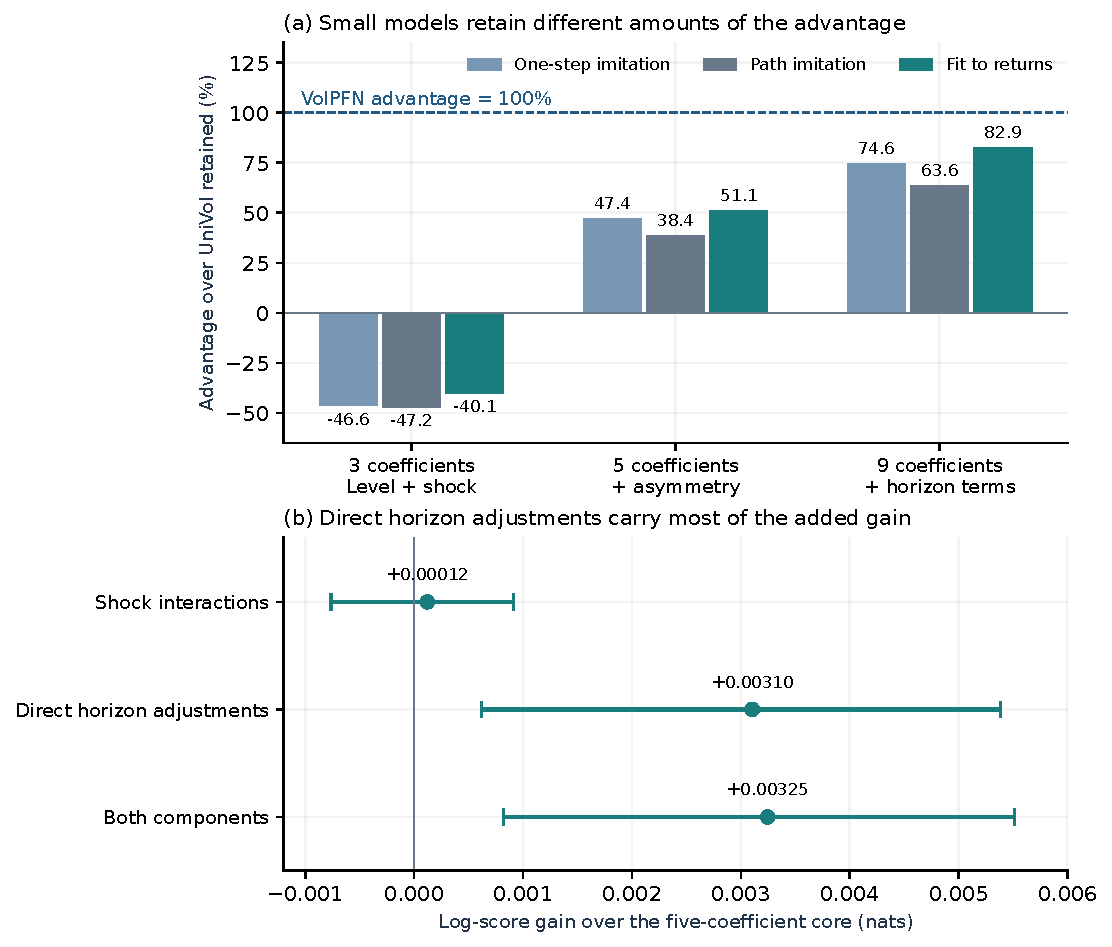
\includegraphics[width=\textwidth]{analysis_compact_rule.pdf}
\caption[Historical compact recovery and driver diagnostics]{Historical development evidence under common-$t_8$ scoring. Top: the original compression study's recovery fractions; 100\% is the retained network's advantage over UniVol, not perfect prediction. Bottom: the separate driver study's attained likelihood-fitted gains over the asymmetric core, with archived marginal 95\% calendar-block intervals. The driver alternatives have unequal optimisation success. Fitting to returns and imitating the network are different objectives; the two nine-coefficient results are separate fits.}
\label{fig:compact-components}
\end{figure}

A large network is therefore not the only way to retain much of this earlier checkpoint's scale performance. The compact evidence supports a predictive alternative while leaving internal computation and full-distribution recovery outside its claim.

\subsection{Supporting checks of objective and prior restriction}

Supporting STES comparisons show that the fitting loss can change the apparent usefulness of horizon inputs: STES changes the weight on recent observations as conditions change. Earlier smaller-network tests also favour completed broad-prior runs, but one broad seed fails, leaving only two genuine broad-versus-narrow pairs. Appendix~\ref{sec:supplementary-analysis} reports both. They motivate caution about objectives and diversity without replacing the five-pair experiment.

\section{Synthetic tracking as a limit on the explanation}

Synthetic tracking tests the stronger explanation that the network follows known variance changes nearly as well as a reference with extra information. Scoring against true simulated variance avoids squared-return proxy noise, although the input returns remain noisy. Up and down jumps have no artificial reflecting boundaries. The defective older lattice reference remains excluded.

Varying change frequency and sequence length gives 170 cells across five seeds. Comparators include compact rules, restarting predictors \citep{herbster1998tracking,hazan2009efficient}, a hindsight-selected filter and a known-model numerical reference. Market-fitted and separately simulation-fitted rules distinguish transfer difficulty from the predictive benefit of refitting the formula.

We exclude the first one hundred observations and compare each forecast with true simulated variance through expected QLIKE:

\begin{equation}
 \sum_{t\geq100}\left\{
 \frac{h_t^*}{\widehat h_t}-\log\!\left(\frac{h_t^*}{\widehat h_t}\right)-1\right\}.
 \label{eq:path-qlike-regret}
\end{equation}

True variance is $h_t^*$ and forecast variance is $\widehat h_t$. The loss compares these quantities directly because the simulation records the variance that generated each return. It thus tests tracking of the simulated state, whereas market QLIKE relies on an observed proxy. Summed path loss is divided by the realised jump count, or one when no jump occurs. This expresses error relative to changes in the tested setting without equalising detection difficulty or quiet-period forecasting cost across lengths.

The references are privileged. The numerical method knows the law and initial state and sets support from the realised path; the fixed filter is chosen with hindsight. Only seven of eighteen simulation-fitted explicit rules converge. These information and fitting differences define the test of the tracking explanation, rather than a comparison of architectures on equal opportunity (Appendix~\ref{sec:supplementary-analysis}).

\begin{table}[!htbp]
\centering
\caption[Synthetic variance-switching results]{Per-jump expected QLIKE loss in the sparse setting $\delta=2$, $V=8$. Each entry averages five paths. The selected lengths illustrate the change across the full prespecified range; smaller is better.}
\label{tab:switching-paths}
\small
\begin{tabular}{lrrr}
\toprule
Forecast & $T=512$ & $T=4{,}096$ & $T=32{,}768$ \\
\midrule
Known-model numerical reference & 15.90 & 18.54 & 26.46 \\
Hindsight fixed-filter selection & 19.15 & 43.57 & 142.38 \\
Restart experts & 22.44 & 31.39 & 52.40 \\
VolPFN & 24.30 & 35.01 & 92.30 \\
Nine-parameter rule, simulation fit & 28.31 & 51.12 & 323.81 \\
Nine-parameter rule, market coefficients & 71.19 & 224.98 & 1,287.94 \\
\bottomrule
\end{tabular}
\end{table}

VolPFN handles long paths better than the market-fitted compact rule, but fails the pre-specified near-reference thresholds. Worst within-window ratios exceed both sparse and dense limits, and the proposed beyond-window deterioration rule also fails. The earlier error-growth claim remains withdrawn: goodness-of-fit values for differently transformed responses cannot distinguish logarithmic from polynomial growth. Appendix~\ref{sec:prior-interpretation-details} records the thresholds and ratios.

\begin{figure}[!htbp]
\centering
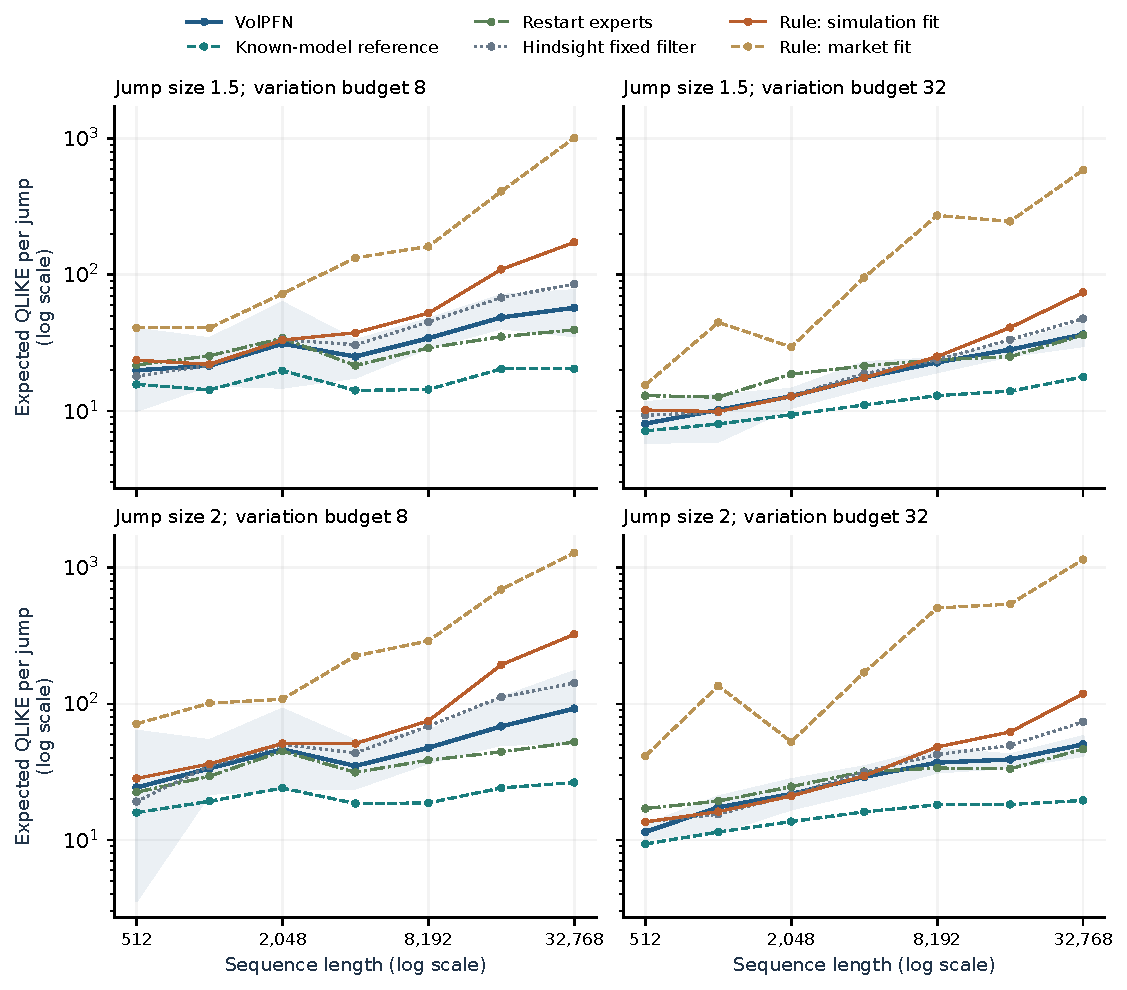
\includegraphics[width=\textwidth]{analysis_tracking_curves.pdf}
\caption[Tracking across the complete sparse sequence-length grid]{Mean per-jump expected QLIKE over five paths at every tested length in all four sparse settings. Lower is better; both axes use logarithmic spacing. The blue band spans the five observed VolPFN values, rather than a confidence interval. The known-model numerical reference and hindsight filter have additional information. The two compact-rule curves use nine coefficients fitted respectively on separate simulations and market data.}
\label{fig:tracking-curves}
\end{figure}

Figure~\ref{fig:tracking-curves} includes every tested sparse-grid length. Refitting improves the compact rule, but neither this nor the network's advantage establishes an asymptotic error rate. Some settings also depart from training in jump size or frequency. The results restrict the tracking explanation without invalidating the separate market comparisons.

The matched-prior gain and compact-rule recovery concern forecast scale. The failed tracking tests limit its proposed explanation. The next chapters examine the remaining prediction question: whether that scale assigns suitable probabilities to extreme losses.

\chapter{Residual correction of VaR and ES}
\label{ch:recalibration}

Widening a predictive distribution does not determine the probability of a severe loss, even when its scale follows the turbulent conditions illustrated earlier. We retain the issued scale and estimate its tail conversion from past outcomes. The procedure below is evaluated in Chapter~\ref{ch:tailresults}.

\section{Why correct the residual tail?}

At level $\alpha$, Value-at-Risk (VaR) defines a return threshold and Expected Shortfall (ES) averages the lowest $\alpha$ fraction of outcomes. Negative returns represent losses. A forecast may follow changing scale while assigning insufficient probability to severe losses, so variance accuracy alone cannot establish accurate VaR and ES.

We take the magnitude of the issued negative VaR as a positive scale and divide each past return by the scale issued before it occurred. Here \emph{residuals} means these standardised outcomes, rather than mean-subtracted regression errors. Their empirical lower quantile and tail average supply the replacement conversion:

\begin{equation}
  \text{new tail pair}=\text{current scale}\times\text{fitted residual tail pair}.
  \label{eq:recal-workflow}
\end{equation}

For example, residual coefficients $-1.2$ and $-1.8$ applied to an original VaR magnitude of $2\%$ give replacement VaR $-2.4\%$ and ES $-3.6\%$. The same coefficients produce smaller losses when multiplied by a quieter day's smaller scale. After warm-up, original ES no longer independently determines the pair. The procedure therefore requires VaR rather than a complete density or standard deviation, although its success still depends on the information retained by that changing scale.

\begin{figure}[!htbp]
\centering
\begin{tikzpicture}[node distance=7mm and 8mm,box/.style={draw=black!45,rounded corners,align=center,text width=3.8cm,minimum height=14mm,font=\small},arr/.style={-{Latex[length=2mm]},thick,draw=black!60}]
\node[box,fill=blue!5] (old) {Past returns and their\\previously issued scales};
\node[box,right=of old,fill=blue!5] (res) {Divide each return by\\its own forecast scale};
\node[box,below=of res,fill=green!5] (tail) {Estimate the residual\\quantile and tail average};
\node[box,left=of tail,fill=green!5] (new) {Multiply both by\\today's forecast scale};
\draw[arr] (old)--(res);\draw[arr] (res)--(tail);\draw[arr] (tail)--(new);
\end{tikzpicture}
\caption[How residual tail correction works]{The correction retains a changing daily scale and estimates the tail from past standardised outcomes. Each scale was issued before its associated return. Forecast ordering and the score's numerical floor are specified in the text.}
\label{fig:tail-correction-workflow}
\end{figure}

With fixed tail shape, this is FHS expressed through VaR \citep{baroneadesi1999var,baroneadesi2008garch}. VaR's fixed multiple of volatility cancels when residual tails are restored to current scale. The forecasts coincide if histories, weights, quantile conventions and safeguards agree. Changing location or shape can break that relationship. Rescaling empirical tails is established; we evaluate its predictive benefit and limits.

\section{How the correction uses past observations}

We retain the original forecast for the first 250 observations. Thereafter, we estimate the residual quantile and integrated tail average before issuing each next pair. After observing the return, we divide it by the original scale issued for that date and add the resulting residual to the history. Keeping those scales preserves the information available at each forecast date. We do not restandardise an earlier return using today's scale, since the residual must measure the outcome relative to the forecast that preceded it.

The integrated average uses exactly the requested sample fraction. For a 1\% tail with 250 residuals, it averages the two lowest values and half the third, dividing by 2.5. Fractional boundary weights prevent excess mass from ties or non-integer tail counts, but create no new observations. Even 500 residuals provide only five observations for a 1\% tail, illustrating the limited severity information at rarer levels.

Numerical safeguards keep ES below VaR and scores finite near zero. These constraints form part of the evaluated procedure; saved losses alone cannot certify that they never activate. Appendix~\ref{sec:tail-score-details} gives their values and the original-model safeguards, and identifies retrospectively fitted, unscored initial histories in some market procedures.

\section{Choosing a history and deciding whether to correct}

Residual-history length controls an estimation trade-off. Full history retains every available residual after initialisation; a rolling window removes older values at a fixed length. More observations may improve precision under stability, but outdated residuals can describe the wrong tail after a change. Shorter windows can adapt sooner while containing fewer extremes. We examine these consequences without assuming an optimal length.

The fixed market study compares full history with 1,000- and 2,000-residual windows. Its \emph{guard} selects correction only when recent mean loss is sufficiently lower than the original forecast's. After 250 post-warm-up comparisons, it checks up to 1,000 past scores against fixed tail-specific margins (Appendix~\ref{sec:tail-score-details}). Both candidates continue updating when unselected, so the next decision can compare their recent performance even if one has not been issued. The guard selects whether to issue the fitted pair; it does not change the residual estimator. Previous performance informs the next choice without guaranteeing improvement.

Development selects the 1,000-residual correction for the later fixed guard. The exploratory selector considers several histories and was designed after evaluation-period exposure. Its additional choices answer a different question and cannot supply independent confirmation. Appendix~\ref{sec:tail-score-details} retains their candidate sets.

\section{What counts as an improvement?}

A breach count measures how often returns fall below VaR, but not how severe those losses are. We therefore assess VaR and ES jointly with FZ0 \citep{fissler2016higher,patton2019dynamic}. For return $y$, threshold $q$, ES $e<0$ and level $\alpha$, the loss is

\begin{equation}
 S_\alpha(y,q,e)
 =-\frac{(q-y)^+}{\alpha e}+\frac{q}{e}+\log(-e)-1,
 \qquad x^+=\max(x,0).
 \label{eq:recal-score}
\end{equation}

We prefer lower FZ0 and interpret differences as loss units, rather than percentages of financial losses avoided. The recorded numerical floor is applied before scoring, with return units fixed within each comparison.

The simulations isolate two consequences of fitting a replacement. Correcting the known true pair measures the cost of estimation when no persistent tail error needs repair. Correcting Gaussian forecasts on heavy-tailed returns measures repair opportunity. Varying path length and changing the law then show how available history and stability affect both. The explanation applies to these settings without supplying a general performance bound.

The grouped comparison examines whether retaining daily scale detail matters. It replaces varying forecasts with one raw-return pair in each scale group, leaving fewer observations to estimate each group's tail. We distinguish online estimates from hindsight fits that use scored outcomes. The comparison follows motivation from \citet{foster2023calibeating} without replicating a general calibration guarantee.

The next chapter measures the benefit of repairing a restrictive tail and the cost of correcting an already accurate forecast. Joint tail scores assess both effects; separate coverage diagnostics assess breach frequency.
\chapter{What tail recalibration improves}
\label{ch:tailresults}

The opportunity for residual correction depends on the original tail forecast. We first test correction against simulated truth, then evaluate it on 28 equity indices. These comparisons show the clearest market benefit for Gaussian tails, while leaving additional neural improvement in the joint score uncertain.

The neural comparisons convert an archived variance path to Student-$t_8$ tails; they use neither the native mixture nor the corrected five-model set. Specialist tables retain their historical fitting policy, with convergence-checked replay reported separately in Appendix~\ref{sec:optimizer-sensitivity}. Prior contact with every market panel remains documented in Section~\ref{sec:exposure}.

\section{Why these comparisons?}

We compare forecasts with different possible errors: Gaussian and Student EWMA, historical simulation, Student GARCH, Gaussian tails on the same GARCH scale, GAS VaR--ES and archived neural variance. FHS supplies the established residual alternative \citep{baroneadesi1999var,baroneadesi2008garch}. Holding GARCH scale fixed across its two tail laws helps distinguish tail-conversion repair from improved volatility prediction.

FZ0 is the main score for the VaR--ES pair at 5\%, 2.5\% and 1\%; breach frequencies and ES residuals are secondary diagnostics. Development covers 2011--2014 and the later panel 2015--February 2022. Paired comparisons give markets equal weight and use synchronised calendar-block intervals. Under the historical protocol, these are marginal intervals rather than joint coverage of all comparisons.

The later evaluation retains the development-selected 1,000-residual guard, even if a different choice appears better afterwards. Appendix~\ref{sec:tail-score-details} records decisions, tolerances and the post-hoc Holm adjustment. Convergence-checked replay on the same observations preserves the principal decisions.

\section{Controlled experiments: correction error and potential benefit}

Simulation provides a reference unavailable in markets: the generating process's true conditional VaR and ES, termed the \emph{oracle}. Correcting this pair tests estimation damage, while correcting a Gaussian forecast tests repair of unsuitable shape. We use stable Student-$t_5$ GARCH, stable Student-$t_5$ switching volatility, and GARCH whose innovations switch halfway from Student-$t_8$ to Student-$t_3$. The 1,620 forecaster, tail, length and seed combinations cover three tail levels, six lengths from 1,000 to 32,000 and five seeds. Scoring starts after 250 observations.

\begin{figure}[!htbp]
\centering
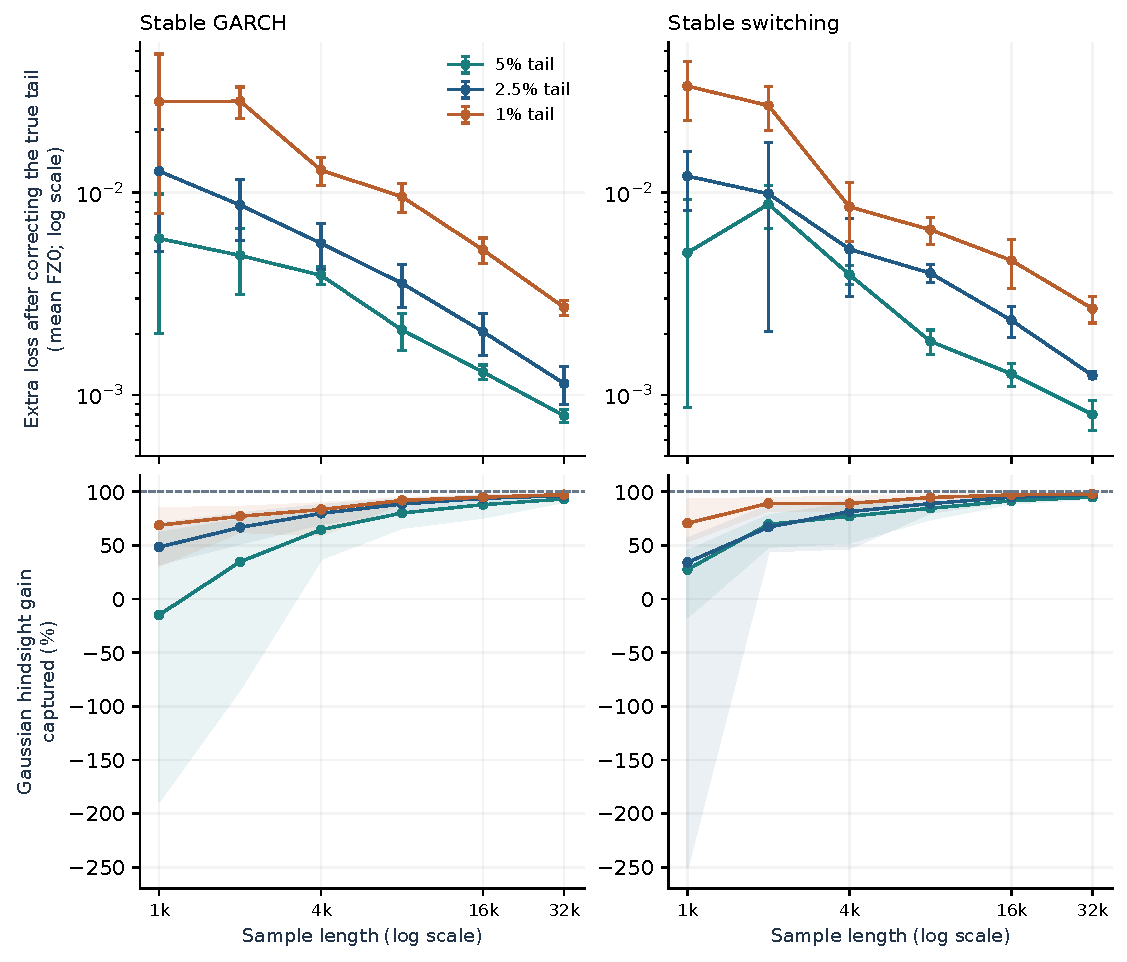
\includegraphics[width=\textwidth]{tail_learning_curves.pdf}
\caption[Tail-correction error and recovered benefit across sample sizes]{Stable Student-$t_5$ simulations at all six scheduled lengths. Top: mean FZ0 increase after correcting the known true tail forecast, with one standard error across five seeds. Bottom: ratio of mean Gaussian-forecast improvement to mean constant-ratio hindsight improvement; shading spans the five individual ratios and the horizontal line marks $100\%$. The hindsight fit uses scored outcomes. These descriptive curves and seed ranges are not confidence bands or general performance guarantees.}
\label{fig:tail-learning}
\end{figure}

As residual history grows, the error introduced by correcting the true forecast generally declines (Figure~\ref{fig:tail-learning}). On long stable paths, Gaussian correction recovers about 93--98\% of the hindsight improvement. The two comparisons show the benefit of repairing Gaussian tails and the estimation cost of correcting the true pair. The recovery ratio divides sample mean gains by a gain from fitting scored outcomes. Small denominators can make the ratio unstable, and realised harm can make it negative. Five seeds describe simulation variation without establishing a universal rate or a market-window choice.

\subsection{Changing tails and the limits of full history}

The halfway law change tests the limitation of full history. Correcting the true pair produces excess losses near 0.005 and 0.007 at 5\% and 2.5\%, exceeding historical tolerance. Pre-change residuals remain in the estimate, so the fitted tail mixes both laws and adapts slowly. Gaussian correction still improves the score over the complete path. This controlled result neither selects an optimal window nor shows that the guard detects a change in time.

\subsection{Retaining the daily scale}

\begin{figure}[!htbp]
\centering
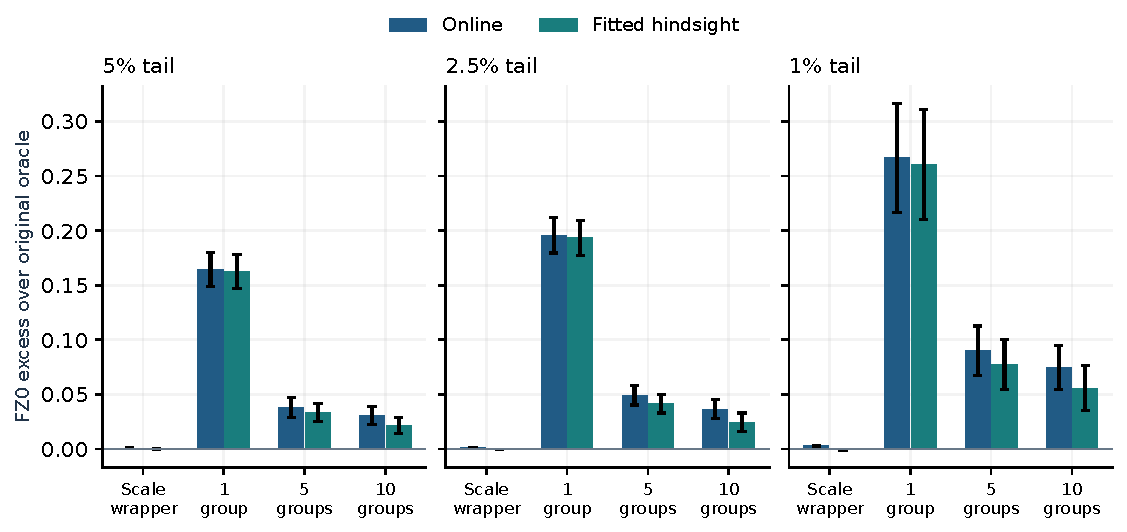
\includegraphics[width=\textwidth]{tail_grouping_cost.pdf}
\caption[What grouping loses when the daily scale is informative]{Stable GARCH oracle at $T=32{,}000$, with five simulation seeds. Bars show mean FZ0 excess over the original oracle; error bars are one standard error across seeds. Online estimates and hindsight fits on the scored sample are separate objects. One, five and ten groups replace the varying scale by constant raw-return pairs within groups; the scale wrapper retains daily scale. Fitted-hindsight excess is not the population approximation floor.}
\label{fig:tail-grouping}
\end{figure}

Grouping replaces each day's changing tail pair with a constant pair within its group. More groups preserve finer scale detail but provide fewer tail observations per estimate (Figure~\ref{fig:tail-grouping}). Online results favour retaining scale in stable GARCH. Hindsight fits see scored outcomes and can fit noise, so their differences measure neither irreducible error nor achievable online gain. The finding concerns these procedures rather than all grouped calibration methods.

\section{Gaussian forecasts: the clearest improvement}

The Gaussian comparison asks whether the guard improves on each original tail pair on the same market observations. Gains are original minus guarded FZ0, so positive values favour correction. Each panel combines two base models and three tail levels.

\begin{table}[htbp]
\centering
\caption[Historical Gaussian-tail improvements and multiplicity]{Historical fixed-guard Gaussian comparisons. Gains are original minus guarded FZ0; positive is favourable. Holm-adjusted $p$-values adjust the six Gaussian-tail comparisons within each panel, post hoc. GARCH rows retain the original optimiser acceptance policy; the convergence-checked sensitivity is separate.}
\label{tab:tail-m1}
\small
\begin{tabular}{llrrrrr}
\toprule
Panel & Base model & $\alpha$ & Gain & Improved & Raw $p$ & Holm $p$\\
\midrule
Development & EWMA Gaussian & .050 & .0266 & 26/28 & .025 & .100\\
 & GARCH Gaussian & .050 & .0045 & 21/28 & .365 & .365\\
 & EWMA Gaussian & .025 & .0659 & 27/28 & .004 & .020\\
 & GARCH Gaussian & .025 & .0173 & 19/28 & .127 & .254\\
 & EWMA Gaussian & .010 & .1613 & 25/28 & .001 & .006\\
 & GARCH Gaussian & .010 & .0534 & 20/28 & .049 & .147\\
\midrule
Later & EWMA Gaussian & .050 & .0297 & 26/28 & .004 & .012\\
 & GARCH Gaussian & .050 & .0035 & 17/28 & .136 & .136\\
 & EWMA Gaussian & .025 & .0878 & 26/28 & .0005 & .003\\
 & GARCH Gaussian & .025 & .0236 & 23/28 & .005 & .012\\
 & EWMA Gaussian & .010 & .2485 & 27/28 & .0005 & .003\\
 & GARCH Gaussian & .010 & .1075 & 26/28 & .0005 & .003\\
\bottomrule
\end{tabular}
\end{table}

Holm adjustment across the six later Gaussian comparisons supports five improvements (Table~\ref{tab:tail-m1}). Gaussian GARCH at 5\% fails both improvement and gain-capture requirements. Development is less supportive: only Gaussian EWMA at 2.5\% and 1\% survives adjustment. Convergence-checked replay retains these decisions.

Correcting Gaussian EWMA and GARCH produces large later 1\% loss reductions, compared with the much smaller neural change (Figure~\ref{fig:tail-starting-model}). The two GARCH versions share variance, making the pattern consistent with repaired tail conversion rather than a better volatility forecast.

\begin{figure}[!htbp]
\centering
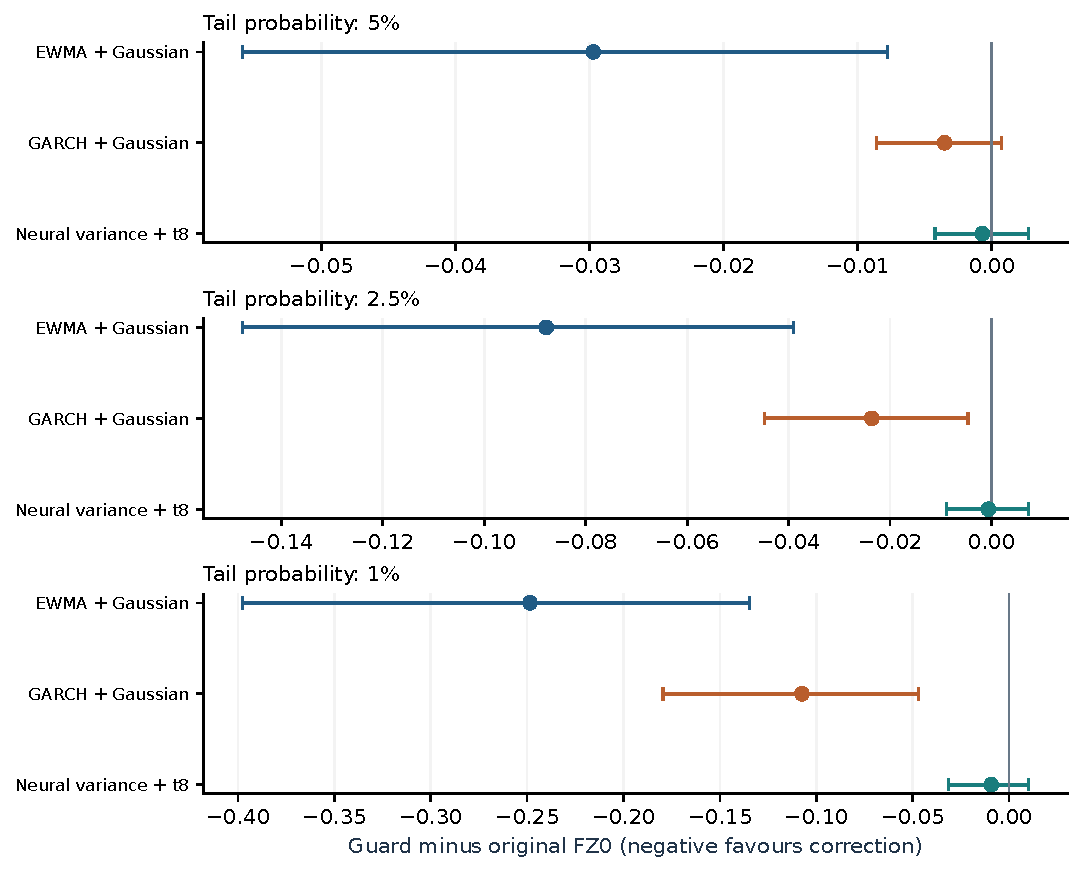
\includegraphics[width=0.94\textwidth]{figures/tail_effect_by_starting_model.pdf}
\caption[Historical tail correction by original forecast]{Historical later-block score changes for the development-selected, 1,000-observation guard. Negative values favour correction. The error bars are the archived individual 95\% calendar-block intervals; the separate Holm adjustment is reported in Table~\ref{tab:tail-m1}. Horizontal scales differ across panels to keep small effects visible. The neural row uses the retained variance path with $t_8$ tails. Specialist rows retain the original optimiser acceptance policy.}
\label{fig:tail-starting-model}
\end{figure}

Gaussian tails leave substantial error to repair here. A more flexible distribution may already capture much of the tail shape, so the gains do not support a universal improvement claim. We next evaluate correction of the archived neural variance forecast with Student tails.

\section{Neural forecasts: coverage improves, score gains remain uncertain}

For the retained neural variance path with Student tails, the table uses corrected-minus-original FZ0: negative differences favour correction. Its marginal intervals concern individual comparisons.

\begin{table}[htbp]
\centering
\caption[Neural-tail joint-score comparisons]{Neural variance with Student-$t(8)$ tails: fixed guard minus original FZ0. Intervals are marginal calendar-block bootstrap intervals, with no multiplicity adjustment.}
\label{tab:tail-neural}
\small
\begin{tabular}{lrrrr}
\toprule
Panel & $\alpha$ & Difference & 95\% interval & Raw $p$\\
\midrule
Development & .050 & +.00019 & $[-.00462,\phantom{-}.00402]$ & .878\\
 & .025 & +.00092 & $[-.00606,\phantom{-}.00629]$ & .716\\
 & .010 & +.00323 & $[-.00170,\phantom{-}.00711]$ & .170\\
\midrule
Later & .050 & -.00071 & $[-.00424,\phantom{-}.00271]$ & .665\\
 & .025 & -.00064 & $[-.00889,\phantom{-}.00722]$ & .872\\
 & .010 & -.00928 & $[-.03137,\phantom{-}.00991]$ & .358\\
\bottomrule
\end{tabular}
\end{table}

Every interval for corrected-minus-original neural FZ0 crosses zero (Table~\ref{tab:tail-neural}). Development means slightly favour the original, and later means favour the guard. Even the later 1\% interval permits benefit or deterioration. The joint-score evidence consequently leaves neural improvement unresolved.

The unconditional breach diagnostic improves more clearly. At the later 1\% level, the number of markets inside the nominal binomial frequency band rises from twelve to 27 of 28, while mean breach frequency falls from about 1.5\% to 1.3\%. Using actual market sample sizes retains that count. These frequencies do not establish conditional coverage, accurate ES or joint-score improvement.

\begin{figure}[htbp]
\centering
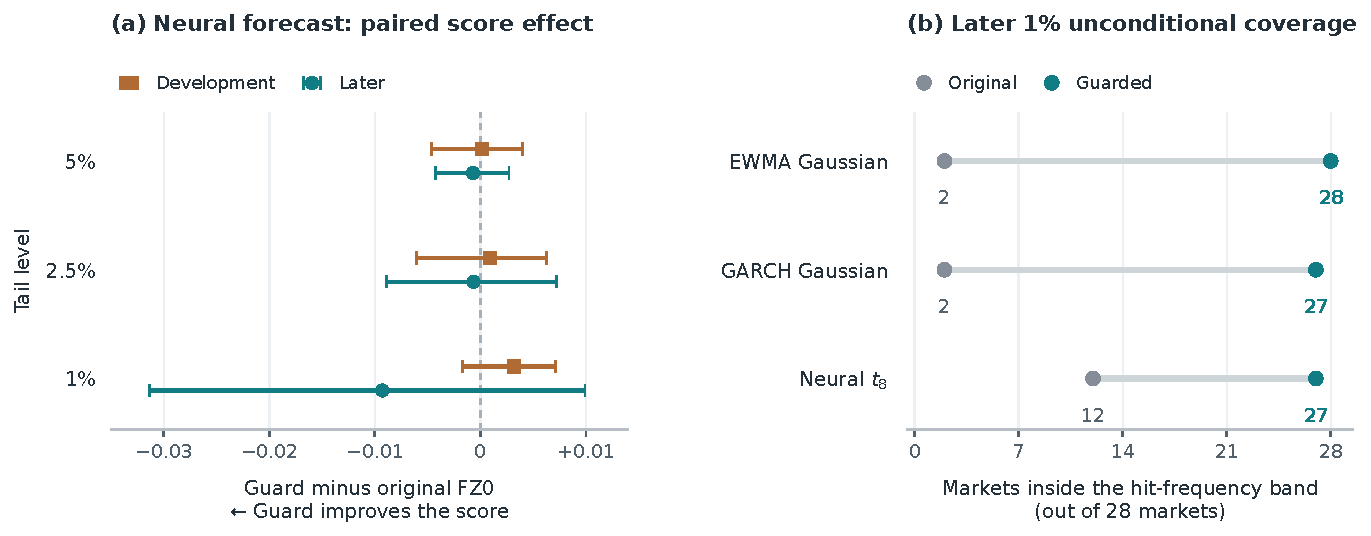
\includegraphics[width=\textwidth]{figures/tail_diagnostics_new.pdf}
\caption[Joint-score uncertainty and unconditional coverage]{Two distinct diagnostics of fixed tail recalibration. (a) Neural variance with Student-$t(8)$ tails: guard-minus-original FZ0 differences and marginal 95\% calendar-block bootstrap intervals. Every interval includes zero. Development uses the full-history guard (\code{guard\_ftl}); the later panel uses the development-selected 1,000-observation guard (\code{guard\_win1000}). (b) Later $1\%$ numbers of markets inside the historical central binomial hit-frequency band before and after that selected guard. The band uses the panel sample-size convention $n=1{,}788$; these are unconditional frequency screens, not conditional coverage tests.}
\label{fig:tail-diagnostics-new}
\end{figure}

Figure~\ref{fig:tail-diagnostics-new} shows this distinction between improved breach counts and uncertain joint scores. Equal counts can also conceal crisis clustering \citep{kupiec1995techniques,christoffersen1998evaluating}. Mean ES residuals decline descriptively, but their archived summaries have no intervals (Appendix~\ref{app:results}). These summaries describe observed severity errors without resolving joint-score uncertainty.

We also assess practical loss tolerances for specialist models. In the convergence-checked later panel, the GAS guard at 1\% exceeds its tolerance. One supplementary unguarded GAS decision at 2.5\% changes from pass to fail, while its guarded counterpart passes. Appendix~\ref{sec:optimizer-sensitivity} separates these changes from the historical tables. Passing a point tolerance is not statistical proof of no harm, and failing it is not statistical proof of harm.

\section{Comparison with filtered historical simulation}

Chapter~\ref{ch:recalibration} shows that fixed-shape ratio correction is FHS expressed through absolute VaR. A claim beyond Gaussian repair therefore requires comparison with FHS. Here FHS refreshes its residual pair at expanding GARCH refits, whereas ratio correction updates sequential residuals daily and the guard may retain the original Gaussian pair. Both updating and selection differ, preventing attribution to selection alone.

\begin{figure}[!htbp]
\centering
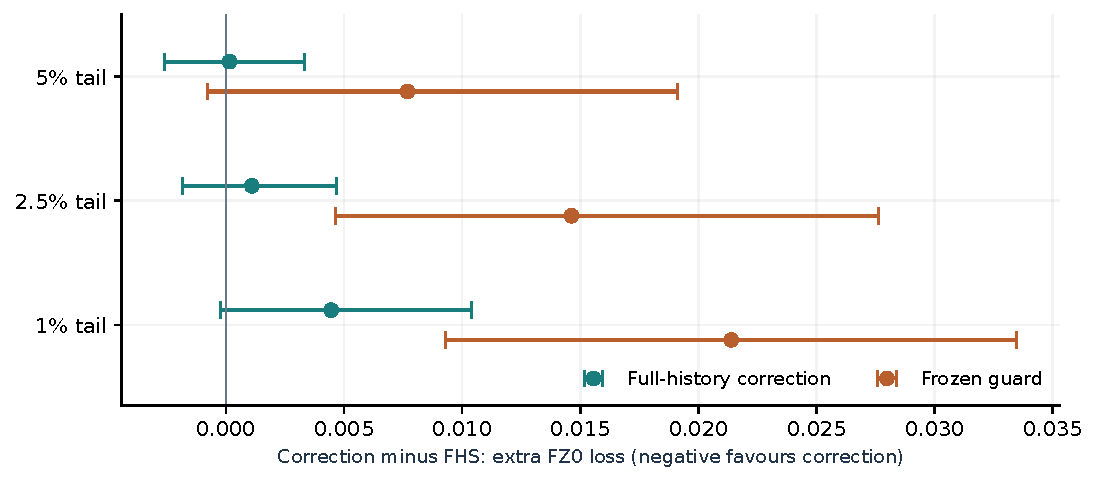
\includegraphics[width=\textwidth]{tail_fhs_comparison.pdf}
\caption[Historical residual correction and guard against FHS]{Historical later 28-market panel: Gaussian-GARCH full-history ratio correction and the frozen guard, each minus GARCH FHS. Positive values mean higher loss than FHS. Bars are archived marginal 95\% calendar-block intervals for these supplementary, post-hoc matched-date comparisons. All GARCH procedures retain the original optimiser acceptance policy. The correction and guard use different residual-history rules, so the comparison does not isolate selection alone.}
\label{fig:tail-fhs}
\end{figure}

On matched dates, full-history correction has similar means to FHS, but all six marginal intervals cross zero. The frozen later guard has higher FZ0 at 2.5\% and 1\%, by about 0.015 and 0.021. These post-hoc comparisons use unadjusted tests, with exact results retained in Appendix~\ref{app:results}. Convergence-checked refitting preserves both findings (Table~\ref{tab:optimizer-fhs-sensitivity}). We establish neither full-history equivalence nor general superiority over FHS.

A guard can avoid an unsuitable correction or discard a useful one (Figure~\ref{fig:tail-fhs}). It must therefore be evaluated as a forecasting procedure, and these results do not generally favour the fixed guard.

\section{Exploratory adaptation and the resulting conclusion}

The exploratory selector chooses among the original and several residual histories. It passes 39 of 57 simulation checks and more later market checks than the fixed guard. However, its design followed inspection of that period; causal updating cannot remove this research exposure. Convergence-checked replay changes no decisions, and Appendix~\ref{app:results} preserves counts and candidates.

Correction helps most clearly with Gaussian tails. Neural joint-score gains remain inconclusive, and the fixed guard sometimes loses to FHS. The simulations show how starting tail error, estimation cost and residual history affect these outcomes within the tested settings; they supply no universal guarantee.

Correction needs to add value over both the original forecast and an established residual alternative. Chapter~\ref{ch:discussion} relates this qualified answer to the prior and compact-recovery findings.
\chapter{Discussion and conclusion}
\label{ch:discussion}

\section{What the completed studies establish}

The matched experiment supports a contribution from the simulated training design: broad training improves on the Mat\'ern alternative under a common law. Benchmarks evaluate the resulting procedures, while historical and intraday controls test explanations of their performance. Fixed ETF evaluation extends the population with mixed comparator outcomes. Compact recovery and tail correction then identify where a large model or another correction adds value, and where support remains limited.

These comparisons answer complementary parts of the overarching question. RQ1 and RQ5 concern performance of issued procedures, RQ2--RQ4 concern training choices and compact recovery, and RQ6 examines the tail limitation of scale prediction. Keeping these roles explicit prevents a successful ranking from becoming an unsupported explanation of why the network works.

\section{Prior design as a modelling contribution}

Holding architecture, initial weights and allocation fixed makes the combined prior design testable. The broad-minus-Mat\'ern gain is about 0.0052 nats per return, with all five pairs and seventeen markets positive. Its small size and concentration also matter: three markets contribute about half of the net gain. The gain is therefore positive in many markets, but modest and uneven.

The prior sets the tasks used to learn a reusable forecasting rule \citep{muller2022transformers}. Our intervention shows that their composition matters relative to the specified alternative, while changing several features together. It cannot identify leverage, switching or return feedback as the cause; those questions need narrower interventions. Nor does it establish that more simulations compensate for an unsuitable task distribution.

The benchmark gains establish usefulness against the specified competitors. Different models and samples prevent assigning those margins to the prior by subtraction, and earlier density findings retain their own checkpoint identity. GP-Vol provides a precedent for flexible dynamics and sequential inference \citep{wu2014gaussian}, but incomplete coverage gives no head-to-head ranking. The contribution remains the evaluated construction and matched training-design result, without depending on new attention machinery, general-purpose inference or verified worldwide priority.

\section{Components, failed configurations and richer information}

The component comparison favours return-distribution prediction over direct expected-squared-return prediction under the tested procedure. Output and loss change together, so neither is isolated. Removing auxiliary simulated-volatility supervision produces no detected deterioration at the recorded weight and budget. These findings identify an effective configuration without establishing that every component is necessary.

The improved historical procedure changes the interpretation of the original training-source comparison. Adding regularisation and development selection reduces mean QLIKE from about 221 in the failed run to about 0.60 on the same index observations. Synthetic means remain slightly lower, but both adjusted probabilities are about $p=0.08$ and both family intervals cross zero. Historical training is therefore competitive. The original underprediction remains a run-specific diagnostic; changing dropout, selection and source together does not identify one cause of its recovery.

The intraday blend adds information from earlier realised kernels and fits their contribution alongside daily risk. Its October controls test whether TTM-only calibration accounts for the observed advantage. Neither the level-and-slope control nor the scale-only control recovers the blend's performance at either proxy; all four comparisons have positive family intervals and retain support under the alternative block lengths. The blend outperforms those controls under their family rules, but its rank among the stronger intraday predictors remains unresolved. GNNHAR retains lower descriptive losses, principal stronger comparisons remain inconclusive, and warm-up forecasts differ. Pooled fitting and unverified RK vintages limit causal interpretation. The cross-market helper still lacks a comparison holding other settings fixed while removing foreign inputs.

The ETF evaluation transfers original weights to a fixed new population. Noaux improves on the stronger historical procedure by about 0.021 QLIKE units, with a positive family interval, five positive seed means and eighteen positive ETF means. Full and noaux also have lower means than rolling GJR, but fail the primary support rule. This supports one training-procedure contrast rather than another broad--Mat\'ern intervention. Unverified human exposure and shared calendar shocks prevent treating it as untouched independent confirmation.

\section{What the simpler rule explains}

Fitting the nine-parameter rule directly to returns retains about 83\% of the earlier network's development advantage over UniVol, after which the rule runs independently. A small predictor therefore retains much of its useful scale performance. Imitation fits recover less, and similar average scores would not establish similar internal computation.

Horizon terms allow the rule to respond when recent variation differs from slower variation. Their attained gain over the converged asymmetric core is consistent with component and HAR-style ideas \citep{engle1999permanent,corsi2009simple}. However, unequal convergence across expanded specifications prevents an intrinsic driver-class ranking. The synthetic stress tests also reject the proposed near-reference tracking explanation, while finite length curves establish no asymptotic error rate.

Compact recovery does not contradict prior contribution. A useful predictor learned from simulation can later have much of its observed advantage retained by a smaller fitted rule. Learning from simulated tasks and fitting compact coefficients to market returns place the assumptions and estimation costs at different stages. Their comparison depends on predictive performance under the stated design rather than parameter count alone.

\section{Why tail correction helps selectively}

FHS separates changing scale from the empirical distribution of standardised residuals \citep{baroneadesi1999var}. We evaluate both the repair this permits and the estimation error it introduces. We score VaR and ES jointly because improved breach frequency alone does not establish better severe-loss prediction \citep{fissler2016higher,patton2019dynamic}.

The clearest correction gains occur with Gaussian tails. Neural joint-score gains remain inconclusive, and the fixed guard sometimes performs worse than FHS. Convergence-checked refitting retains these principal conclusions while changing one supplementary tolerance decision for unguarded GAS.

The simulations explain why the benefit is conditional. Estimating a new tail can damage a correct forecast, with that cost declining as stable history grows. After a shape change, old residuals delay adaptation. These controlled examples connect the market findings to starting error and available information, but select neither an optimal market window nor a universally improving correction.

\section{Limits of the conclusions}

\paragraph{Data exposure and population.}
Prior index-data contact remains documented in Section~\ref{sec:exposure}; later freezes constrain choices without undoing exposure. The ETF protocol preceded acquisition, but prior human exposure is unverified and its dates share index-study shocks. Index exclusions, the fixed ETF roster and the open-to-close target define our population. External-pretraining overlap remains unknown, preventing a claim that every evaluated observation was unseen by every pretrained competitor. Source revisions and RK publication vintages also remain incompletely resolved, so chronological indexing alone cannot certify what data were available at the time. These limits restrict generalisation, and the evaluation establishes neither overnight portfolio performance nor trading returns.

\paragraph{Attribution and comparison scope.}
The changes controlled in each comparison determine what it can explain. Prior matching changes several simulation ingredients together, while distribution-versus-direct changes both output and loss. Benchmark contexts, selection opportunities and median or mean outputs also differ, so the rankings cannot isolate architecture. Within VolPFN, auxiliary labels omit some covariances and masked training does not target the complete zero-inclusive simulator law. The compact and tail findings also concern an earlier checkpoint. Calibration can adjust forecast level without aligning native objectives, and RK has not been equated to next-session return risk. These differences limit what each result can attribute to an individual modelling choice.

\paragraph{Conditional inference and selection.}
Calendar intervals measure date variation conditional on the saved forecasts, markets and masks. They do not repeat training, calibration or online fitting within each resample, and therefore omit that estimation uncertainty as well as research-selection uncertainty. Five seeds help describe consistency across training runs without covering every possible run. Selection history also matters: the historical analysis specification was recorded after its first seed result became visible, so the documented freezes are not formal preregistration. Finally, adjustment within separate families gives no dissertation-wide multiplicity guarantee, and correlated market signs cannot be counted as independent replications.

\paragraph{Simulation transfer and numerical estimation.}
Simulation findings apply to the stated processes, lengths and seeds, with privileged references and finite ranges limiting market transfer. Solver convergence establishes neither a global optimum nor freedom from numerical safeguards. Floors and retrospectively fitted, unscored prefixes remain part of the tail procedures; saved losses cannot show that constraints never activate. Causal updating establishes information order rather than calibration or improvement.

\section{Conclusion}

The five matched broad--Mat\'ern pairs support a modest contribution from the combined simulation design. The result answers the prior question at that level, leaving individual causal ingredients unidentified.

VolPFN ranks first in the tested general pretrained benchmark, and its variants lead the daily-return-only leaderboard of dedicated financial models and general pretrained forecasters. Leadership describes the evaluated procedures and does not establish adjusted superiority over every competitor. Distribution prediction outperforms direct risk prediction; extra volatility supervision has no detected benefit; and the stronger historical procedure is competitive on indices. The intraday blend improves on TTM-only calibration controls, while stronger alternatives remain unresolved. Fixed ETF evaluation supports noaux over the improved historical procedure, but leaves superiority over rolling GJR inconclusive.

A compact rule independently retains much of the earlier checkpoint's scale advantage. This supports a simpler predictive alternative without explaining the network's computation.

Residual correction adds value most clearly for Gaussian tails. Additional neural joint-score gains remain uncertain, and the fixed guard sometimes loses to FHS. Its value therefore depends on the original forecast and the evidence available for estimating a replacement.

The synthetic design contributes to prediction in the evaluated comparisons, subject to the documented exposure and conditional uncertainty. The results support forecasting performance and a contribution from the combined training design. They do not explain the network's internal mechanism.

\begingroup
\raggedright
\bibliographystyle{plainnat}
\bibliography{refs,refs_background_additions,refs_design_additions,refs_methods_condensed,refs_research_additions}
\endgroup
\begin{appendices}
\chapter{Technical specification and evaluation protocol}
\label{app:technical}
\label{app:forecast-details}
\label{app:closure_protocol}

These records supplement the methods in Chapters~\ref{ch:data}--\ref{ch:analysis}. Training design v2 and prior/benchmark plans v3 define the corrected studies; retained-checkpoint studies keep their earlier identity.

\section{Reference models and scoring}
\label{sec:appendix-reference-models}

GARCH uses mean $\mu$, forecast variance $h_t$ and zero-mean, unit-variance innovations $\eta_t$:
\begin{equation}
 r_t=\mu+\sqrt{h_t}\,\eta_t,\qquad
 h_t=\omega+a(r_{t-1}-\mu)^2+b h_{t-1}.
 \label{eq:appendix-garch}
\end{equation}
The density benchmark uses Student innovations, a 1,000-observation fitting window and 250-observation refits. EWMA uses $\lambda=0.94$:
\begin{equation}
 h_{t+1}=\lambda h_t+(1-\lambda)r_t^2.
 \label{eq:appendix-ewma}
\end{equation}
Log density is scored by $\log p_t(r_t)$; QLIKE scores a positive second-moment forecast:
\begin{equation}
 \ell_Q(r_t,h_t)=\frac{r_t^2}{h_t}+\log h_t.
 \label{eq:appendix-qlike}
\end{equation}
Second moment equals variance under zero mean. Synthetic excess QLIKE is given in equation~\eqref{eq:path-qlike-regret}.

For likelihood training, each unmasked target receives reciprocal batch-mask-count weight; masked targets and empty batches contribute zero. Thus a target's contribution depends on how many positions are scored in its batch, not only on whether it is selected. Averaging these weighted input--target pairs over batches and normalising total weight defines the scored-position distribution. An unrestricted likelihood-only predictor would target its conditional next-return law given bounded-context features and base scale. This need not equal the unweighted simulator's fresh-observation law because batch denominators vary. The mask selects loss positions, without supplying future information. Finite features, clipped Student outputs and joint auxiliary training restrict this idealisation; the continuous mixture cannot represent the simulator's point mass at zero. This likelihood target does not establish that the prior correctly describes markets.

\section{Simulation and causal inputs}

The prior $\Pi$ selects process family $F$ and parameters $\psi$, generating returns from variance $v_t$ and standardised shocks:
\begin{equation}
 r_t=\sqrt{v_t}\,\epsilon_t,\qquad
 (F,\psi)\sim\Pi,\qquad
 \E(\epsilon_t)=0,\quad \E(\epsilon_t^2)=1.
 \label{eq:volpfn-simulation}
\end{equation}
Gaussian innovations have probability 0.25; otherwise degrees of freedom are log-uniform on $[2.5,50]$. Symmetry has probability 0.75; otherwise the Fern\'andez--Steel skew parameter is log-uniform on $[0.7,1.4]$, followed by zero-mean, unit-variance standardisation. Stale observations report zero until accumulated returns are released; zero targets are masked.

The running nonzero-return RMS $s_t$ uses the current window through $t$, or one before its first nonzero return. Input $x_t=r_t/s_t$ predicts $r_{t+1}/s_t$ and auxiliary label $\log v_{t+1}-2\log s_t$. Raw-unit negative log density adds $\log s_t$. Scale and moment states reset by window; float64 log accumulation precedes float32 network inputs.

\begin{table}[htbp]
\centering\small
\caption[The eight causal input channels]{Input transformations in the corrected procedure. The moment $e^{\rm raw}_{j,t}$ is calculated in raw-return units; $t$ is the zero-based position within the window.}
\label{tab:appendix-input-channels}
\begin{tabular}{@{}p{3.2cm}cp{8.8cm}@{}}
\toprule Quantity & Channels & Value supplied \\
\midrule
Scaled return & 1 & $\operatorname{asinh}(x_t)$ \\
Squared-return magnitude & 1 & $\log(x_t^2+10^{-6})/4$ \\
Stale-return flag & 1 & One when $r_t=0$, otherwise zero \\
Return sign & 1 & $\operatorname{sign}(r_t)$ \\
Exponential second moments & 3 & $(\log e^{\rm raw}_{j,t}-2\log s_t)/4$, with half-lives $j=5,20,100$ \\
Window position & 1 & $\log(1+t)/8$ \\
\bottomrule
\end{tabular}
\end{table}

Each raw moment starts at one, takes the first nonzero return's square, then weights its preceding value by $2^{-1/j}$ and the new square by $1-2^{-1/j}$. Zeros leave it unchanged. Legacy training instead uses nonzero RMS from the first 100 positions, allowing later synthetic observations to affect early units, with moments initialised at one in normalised units. Historical market inference uses an available prefix.

\subsection{Parameter draws defining the broad prior}

$U(a,b)$ is uniform, $\operatorname{LogU}(a,b)$ is uniform in log units before exponentiation, and $N(\mu,\sigma^2)$ is normal with mean $\mu$ and variance $\sigma^2$. Here $\theta_t=\log v_t$. GJR's $\kappa$ is the negative-shock second moment; EGARCH's $m_1$ is mean absolute shock. SV uses independent standard-normal $\xi_t$. GARCH/GJR/EGARCH start at log variance $N(0,0.6^2)$, with a 300-step burn-in with probability 0.5 and none otherwise. Each history receives new parameters from \code{volpfn\_prior.py}.

\begin{longtable}{@{}>{\raggedright\arraybackslash}p{2.0cm}>{\raggedright\arraybackslash}p{11.8cm}@{}}
\caption[Broad-prior parameter draws]{Family parameter distributions and recursions. Family-selection probabilities remain those in Table~\ref{tab:simulation-prior}.}\label{tab:prior-parameter-draws}\\
\toprule Family & Draws and dynamics \\
\midrule
\endfirsthead
\toprule Family & Draws and dynamics \\
\midrule
\endhead
GARCH & $1-P\sim\operatorname{LogU}(0.001,0.15)$, $a=P U(0.02,0.30)$, $b=P-a$, $\omega=1-P$. Update $v_{t+1}=\omega+a v_t\epsilon_t^2+bv_t$. \\
GJR & Same $P$, with $a=P U(0,0.20)$ and $g=P U(0.02,0.35)$. Let $\kappa=\E[\epsilon_t^2\ind\{\epsilon_t<0\}]$, computed analytically for the centred innovation law. Set $b=P-a-g\kappa$, $\omega=1-P$ and update $v_{t+1}=\omega+(a+g\ind\{\epsilon_t<0\})v_t\epsilon_t^2+bv_t$. \\
EGARCH & $1-b\sim\operatorname{LogU}(0.003,0.15)$, $a\sim U(0.05,0.30)$, $g\sim U(-0.25,0.05)$. Update $\theta_{t+1}=b\theta_t+a(|\epsilon_t|-m_1)+g\epsilon_t$, with $m_1$ estimated from 20,000 independent innovation draws. \\
SV & $1-\phi\sim\operatorname{LogU}(0.002,0.10)$, $d\sim U(0.3,1.5)$ and $s_w=d\sqrt{1-\phi^2}$. With probability 0.6, $\rho\sim U(-0.8,0.2)$; otherwise $\rho=0$. Start $\theta_0\sim N(0,d^2)$; update $\theta_{t+1}=\phi\theta_t+s_w(\rho\epsilon_t+\sqrt{1-\rho^2}\xi_t)$, $\xi_t\sim N(0,1)$. \\
Rough & Independently uniform choices $H\in\{0.05,0.10,0.20,0.35,0.50\}$ and $\ell\in\{30,120,500\}$; $d\sim U(0.3,1.5)$. Draw a stationary Gaussian log-variance path with Mat\'ern covariance and standard deviation $d$ by finite circulant embedding. Negative embedding eigenvalues, if any, are clipped to zero. \\
HMM & Uniform choice $K\in\{2,3\}$, $d\sim U(0.4,1.2)$; draw $K$ levels from $N(0,d^2)$, sort and subtract their mean. Independent durations $D_k\sim\operatorname{LogU}(20,1500)$ give $P_{kk}=1-1/D_k$ and $P_{kj}=1/[D_k(K-1)]$ for $j\ne k$. The initial state is uniform over the $K$ levels. \\
Lattice & $K\sim U(2,25)$ and $\delta\sim U(0.3,1.5)$. Start $\theta_0=0$; at subsequent positions, move by $+\delta$ or $-\delta$ with equal probabilities conditional on a move, whose probability is $K/T$. Reverse a proposed step if it would exceed $[-3.5,3.5]$. \\
\bottomrule
\end{longtable}

Modifications activate independently and follow the table's order. Return jumps use Bernoulli events, not compound Poisson counts.

\begin{longtable}{@{}>{\raggedright\arraybackslash}p{2.0cm}>{\raggedright\arraybackslash}p{11.8cm}@{}}
\caption[Broad-prior modification draws]{Modification parameters in \texttt{apply\_overlays}. The variance label is modified as indicated; this is an inherited approximation when autoregression and stale aggregation coexist.}\label{tab:prior-overlay-draws}\\
\toprule Overlay & Draws and effect when active \\
\midrule
\endfirsthead
\toprule Overlay & Draws and effect when active \\
\midrule
\endhead
Return jumps (0.30) & $\lambda\sim\operatorname{LogU}(0.002,0.05)$, $k\sim U(3,10)$. Add $\sqrt{v_t}B_t Z_t$, with $B_t\sim\operatorname{Bernoulli}(\lambda)$ and $Z_t\sim N(0,k^2)$ independently. The label is multiplied by $1+\lambda k^2$. \\
Return AR (0.30) & $\rho\sim U(-0.15,0.15)$; recursively replace the return by $r_t+\rho r_{t-1}$, starting with previous return zero. The variance label is unchanged at this stage. \\
Drift (0.50) & Draw one $\mu\sim N(0,0.03^2)$ per history and add it to every return in simulator units. The variance label is unchanged. \\
Stale prices (0.25) & $q\sim\operatorname{LogU}(0.005,0.20)$ and $m\sim U(1,4)$. A two-state chain starts fresh before its first transition, with fresh-to-stale probability $q/[m(1-q)]$ and stale-to-fresh probability $1/m$. Stale days report zero; the next fresh day reports the sum since the previous fresh day. Labels on fresh days sum the corresponding variances using log-domain aggregation; covariance terms from return AR are omitted. Trailing unreleased stale intervals are not reported. \\
\bottomrule
\end{longtable}

Labels include jump variance and released-interval variance sums, omitting AR covariance terms. They need not equal unmodified diffusive variance or the return second moment conditional on observed history.

\section{Attention, predictive output and objective}

The corrected transformer has six blocks, width 256, eight attention heads and 4,746,002 parameters. Each head has 32 coordinates, and feed-forward layers expand 256 to 1,024 and back. Capacity is fixed across prior configurations and has not been established as optimal.

For query $q_t^{(a)}$, key $k_j^{(a)}$, head dimension $d_a$ and distance slope $m_a$, causal attention weights are normalised over $j\leq t$:
\begin{equation}
 A_{t,j}^{(a)}\ \propto\
 \exp\!\left(\frac{q_t^{(a)\top}k_j^{(a)}}{\sqrt{d_a}}-m_a(t-j)\right),
 \qquad j\leq t.
 \label{eq:volpfn-attention}
\end{equation}
The dot product measures the query--key match, while the distance term changes the weight assigned to older positions before normalisation. Future weights are zero, so neither term admits a later observation into the current prediction. Seven slope exponents span $-1$ to $-10$ equally; the eighth is zero, a custom ALiBi-based schedule \citep{press2022alibi}. Pre-normalised residual attention/feed-forward blocks use GELU, with no dropout, separate encoder, cross-attention or added positional embedding.

For $e_{20,t}=e^{\rm raw}_{20,t}/s_t^2$ and $s_{20,t}=\sqrt{e_{20,t}}$, network outputs $a_k,b_k,c_k$ become Student locations, scales and degrees of freedom:
\[
 \mu_{k,t}=s_{20,t}a_{k,t},\quad
 \log s_{k,t}=\log s_{20,t}+\operatorname{clip}(b_{k,t},-6,6),\quad
 \nu_{k,t}=2.1+\exp\{\operatorname{clip}(c_{k,t},-4,6)\}.
\]
Softmax weights $w_{k,t}$ give equation~\eqref{eq:volpfn-density}. Student scale differs from standard deviation; the second moment is
\begin{equation}
 h_{t+1}=\sum_k w_{k,t}\left\{
 s_{k,t}^{2}\frac{\nu_{k,t}}{\nu_{k,t}-2}+\mu_{k,t}^{2}\right\}.
 \label{eq:volpfn-second-moment}
\end{equation}
Each component contributes its variance and squared centre to the second moment, weighted by its mixture probability. Central variance then subtracts squared predictive mean. This distinction matters when the mixture mean is not zero. Common-$t_8$ scoring uses scale $\sqrt{6h/8}$, suppressing GARCH's fitted mean without equating its variance to the other methods' second moments.

The auxiliary Gaussian has learned mean $m_t=\log e_{20,t}+\delta_t$ and standard deviation $u_t$, with $\log u_t$ clipped to $[-5,3]$. Targets are $\widetilde r_{t+1}=r_{t+1}/s_t$ and $\widetilde\ell_{t+1}=\log v_{t+1}-2\log s_t$; $M_{t+1}$ marks scored positions:
\begin{equation}
 \mathcal L=
 \frac{\sum_t M_{t+1}\left[-\log q_t(\widetilde r_{t+1})+
 0.1\left\{\frac{(\widetilde\ell_{t+1}-m_t)^2}{2u_t^2}+\log u_t\right\}\right]}
 {\max(1,\sum_t M_{t+1})}.
 \label{eq:volpfn-training-details}
\end{equation}
The sum covers the whole minibatch, not separately normalised histories. The Gaussian constant is omitted; corrected raw-unit loss adds the scale Jacobian. The auxiliary head's implied mean variance $\exp(m_t+u_t^2/2)$ is unused at evaluation. Its Gaussian likelihood supervises the simulated log-variance target; the Student mixture supplies the return density and the moments used in forecast comparisons. Component comparisons and the unvalidated 0.1 weight are discussed in Section~\ref{sec:new-components}.

\section{Frozen training and checkpoint provenance}

\begin{longtable}{@{}>{\raggedright\arraybackslash}p{4.0cm}>{\raggedright\arraybackslash}p{9.8cm}@{}}
\caption[Matched training specification]{Training settings shared by the broad and Mat\'ern arms.}\\
\toprule Setting & Frozen value \\
\midrule
\endfirsthead
\toprule Setting & Frozen value \\
\midrule
\endhead
Network & Width 256; six blocks; eight attention heads; four Student-$t$ components; eight input channels. \\
Loss & Return-density loss plus auxiliary log-variance loss, weight 0.1; inherited overlay-label approximation disclosed. \\
Budget & 20,000 updates; 8,192 input positions per update; 163,840,000 total positions per model. \\
Sequence lengths & 512 with probability 0.4; 1,024 with probability 0.6. \\
Optimiser & AdamW; learning rate 0.0003; warm-up 300 updates; $\beta=(0.9,0.98)$; weight decay 0.01; $\epsilon=10^{-8}$; gradient-norm clip 1.0. \\
Features and scale & Running nonzero RMS within each window; unit scale before a nonzero return; EWMA half-lives 5, 20 and 100; states reset per window. \\
Shared overlays & Jump probability 0.30; autoregression 0.30; drift 0.50; stale observations 0.25. Innovation-law sampling is shared. \\
Broad family weights & GARCH 0.20; GJR 0.15; EGARCH 0.10; SV 0.20; rough 0.10; HMM 0.12; lattice 0.13. \\
Mat\'ern package & Uniform choice from nine smoothness/length-scale pairs: smoothness $0.1,0.5,1.5$; length scale $30,120,500$; log-variance standard deviation uniform on $[0.3,1.5]$; stationary finite-dimensional Gaussian draw. \\
Numerical backend & RTX 4090; Python 3.12.3; NumPy 1.26.4; SciPy 1.13.1; PyTorch 2.8.0+cu128; CUDA 12.8; float32; deterministic algorithms; no autocast or TF32. \\
Data pipeline & Two workers; four prefetched batches; seed/update-indexed generation; two computational threads. \\
Validation & Every 500 updates; 48 series of length 1,024 per diagnostic panel; 100-step burn; validation seeds 99101/99102/99103 for broad/GARCH/Mat\'ern. \\
Checkpoint rule & Fixed final at update 20,000 only. Intermediate saves every 2,500 updates; no validation-based final selection. \\
Failure rule & Preserve failed attempts; no replacement seed or survivor-only primary. Technical continuations require a separate provenance record. \\
\bottomrule
\end{longtable}

Cosine decay follows warm-up. Interval-local stale aggregation and analytic centred skew-$t$ GJR semivariance repaired earlier simulation. All broad models restarted; Mat\'ern seeds 8101/8102 were reused after dependency and finite-state checks, without full GPU replay. The AR--stale label approximation remains.

\begin{table}[htbp]
\centering\small
\caption[Five-pair checkpoint provenance]{All eligible pairs. Hash prefixes identify checkpoint files for readable cross-reference; complete SHA-256 values and initial-state hashes are in the registry. Every within-pair initial-state hash agrees.}
\label{tab:closure_provenance}
\begin{tabular}{@{}lp{4.2cm}p{4.2cm}p{3.5cm}@{}}
\toprule Seed & Broad final & Mat\'ern final & Provenance \\
\midrule
8101 & \texttt{f1bd7c9bddb0} & \texttt{12052313f91d} & Broad fresh; Mat\'ern reused \\
8102 & \texttt{2b8ed9e7662d} & \texttt{6e90b215948d} & Broad fresh; Mat\'ern reused \\
8103 & \texttt{7fd7d9496b37} & \texttt{595c38ba0c7c} & Both fresh \\
8104 & \texttt{c431c649fb03} & \texttt{8f495bea58b7} & Both fresh \\
8105 & \texttt{1bf94170feb4} & \texttt{54747a95a5e8} & Both fresh \\
\bottomrule
\end{tabular}
\end{table}

Training/prior plans froze on 19 September 2026 at 12:45:43 UTC, benchmark at 12:45:45. Training hash prefixes are \texttt{46eb1e39aaeb} (v2) and \texttt{bc0074408470} (reused v1). Earlier seed-8101 results were exposed.

\section{Data eligibility and excluded indices}

Chapter~\ref{ch:data} states the inclusion gate. Comparable finite positive prices use relative/absolute equality tolerances $10^{-10}/10^{-12}$; same-day open/close equality is descriptive. Fewer than twenty qualifying markets makes the endpoint unavailable; substitutes and close-to-close fallback are prohibited.

AEX, BFX, BSESN, DJI, FCHI, GDAXI, GSPTSE, HSI, IBEX, IXIC, KS11, MXX, N225, NSEI, OMXSPI, RUT, SPX, SSEC, SSMI and STOXX50E qualify: 22,541 rows, 1,176 union dates, 1 March 2022--31 August 2026.

\begin{longtable}{@{}>{\raggedright\arraybackslash}p{1.8cm}>{\raggedright\arraybackslash}p{2.3cm}p{1.2cm}>{\raggedright\arraybackslash}p{8.1cm}@{}}
\caption[All eight later-period exclusions]{Excluded candidates under the unchanged data gate. Row counts, where present, describe valid target returns before the market-level exclusion.}\label{tab:closure_exclusions}\\
\toprule Index & Vendor symbol & Rows & Reason for exclusion \\
\midrule
\endfirsthead
\toprule Index & Vendor symbol & Rows & Reason for exclusion \\
\midrule
\endhead
AORD & \texttt{\^{}AORD} & 1,139 & Open equals preceding close in 94.82\% of comparable rows, exceeding 20\%. \\
BVSP & \texttt{\^{}BVSP} & 1,125 & Open equals preceding close in 30.93\%, exceeding 20\%. \\
FTSE & \texttt{\^{}FTSE} & 1,135 & Open equals preceding close in 86.52\%, exceeding 20\%. \\
KSE & \texttt{\^{}KSE} & --- & Specified symbol returned HTTP 404; no substitute. \\
OMXC20 & \texttt{\^{}OMXC20} & --- & Full-history response lacked its timestamp array despite a separate identity response. \\
OMXHPI & \texttt{\^{}OMXHPI} & 0 & No valid primary OHLC rows; day-count, invalid-fraction and comparable-open checks failed. \\
OSEAX & \texttt{OSEAX.OL} & --- & Vendor identifies a GI series; compatibility of the valuation convention remained unresolved. \\
SMSI & \texttt{\^{}SMSI} & --- & Specified symbol returned HTTP 404; no substitute or IBEX replacement. \\
\bottomrule
\end{longtable}

Reconciliation matched 24 timestamp-bearing responses and 100 data-lock hashes. Bounded arithmetic-portability differences leave sealed arrays/masks unchanged. Identity, mapping and data seals date from 19 September at 10:22:16, 10:24:55 and 10:25:28 UTC. Earlier SPX/FTSE/GDAXI/N225 audits and metadata contact remain disclosed; acquired 1 September rows are excluded. These checks do not independently verify exchange prices.

\clearpage
\section{Statistical rules and external-model interfaces}

\begin{longtable}{@{}>{\raggedright\arraybackslash}p{3.15cm}>{\raggedright\arraybackslash}p{5.3cm}>{\raggedright\arraybackslash}p{5.3cm}@{}}
\caption[Final inference rules]{Different endpoints and uncertainty procedures in the two completed comparisons.}\\
\toprule Rule & Matched prior & Corrected benchmark \\
\midrule
\endfirsthead
\toprule Rule & Matched prior & Corrected benchmark \\
\midrule
\endhead
Favourable effect & Broad minus Mat\'ern common-$t_8$ log score & Competitor minus VolPFN fixed-scale QLIKE loss \\
Aggregation & Time within market, equal markets, equal paired seeds & Time within market, equal markets, equal model seeds \\
Scale convention & Raw predictive second moment; no market-fit multiplier & Each model's development-fitted multiplier; competitor multipliers fixed \\
Primary context & Length 1,024; stride 512; minimum history 100 & Per-origin preceding 1,024 observed returns \\
Bootstrap & 5,000 synchronised circular calendar draws; block 60; seed 9182601 & 20,000 synchronised circular calendar draws; block 10; seed 2026091902 \\
Superiority tests & One-sided centred bootstrap; Holm across two reserved contrasts & Two-sided centred bootstrap; Holm across three competitors \\
Intervals & Basic 95\% interval for the primary contrast & Basic marginal intervals at $1-0.05/3$ coverage, yielding approximate family 95\% coverage \\
Decision requirements & Holm $p\leq0.05$; positive 95\% interval; mean at least 0.005 nats; at least 15/20 positive market means & Positive mean; Holm $p\leq0.05$; positive lower family-interval endpoint \\
Unavailable slot & Broad--GARCH remains unrun, $p=1$ in the Holm family & No missing comparator in the completed three-slot family \\
Equivalence & Separate TOST and strict basic 90\% interval inclusion within $\pm0.003$ nats & Not a primary confirmation endpoint \\
Sensitivity & QLIKE and native-density summaries are supporting & Blocks 5 and 20, adjusted separately; native QLIKE and pinball descriptive \\
Not quantified & Training-seed population, prior/research/population selection uncertainty & Training-seed population, calibration estimation and research/population selection uncertainty \\
\bottomrule
\end{longtable}

Bootstrap probabilities use plus-one correction; seeds are not resampled. Block intervals depend on the stated dependence approximation. Prior superiority/equivalence and separately adjusted benchmark sensitivities have no joint guarantee.

Adapters use \code{amazon/chronos-2}, \code{Salesforce/moirai-2.0-R-small} and local TabPFN-TS with \code{tabpfn-v3.5-20260909}; complete revisions/hashes remain in the manifest. TabPFN-TS uses eight estimators and a fixed seed. Chronos/Moirai expose squared-return medians, TabPFN-TS a mean. The floor is $\max(10^{-12},10^{-8}\times\text{context mean square})$; rearranged raw-return quantiles are flagged.

Development multipliers are 4.1835301, 4.2152974 and 1.3698467, respectively. Each VolPFN seed fits its own multiplier on the same 72 origins, equally averaging observed-square/prediction ratios by market. Each model supplies 8,774 evaluation and 72 calibration predictions. An exact 50-row bridge verifies the resumed calculation; saved masks/hashes are authoritative.

\subsection{Common-period units and scored moments}
\label{sec:common-period-units}

Intersecting locked masks gives 22,026 keys and 827 union dates in 2019--February 2022. Alignment involves no retraining or recalibration and does not remove unfavourable forecasts. Decimal returns convert to percent once, decimal RK to percent-squared by 10,000 once; already converted moments remain unchanged.

Squared-return scoring uses second moment; harmonised, intraday and helper RK scoring uses central variance, differing by squared predicted mean. The original secondary RK diagnostic instead uses moment and remains distinct. Direct has only second moment, not native density or separately identified variance. Common-$t_8$ scoring does not make it a trained density model.

Standalone VolPFN uses daily returns. Intraday helpers add lagged RK; GNNHAR and Transfer-XGBoost add foreign histories, while blend fitting pools completed market--days. These procedures differ in information and fitting as well as architecture. Session chronology establishes neither RK publication/vintage availability nor equivalence to session return risk.


\section{Compact rules and fitting objectives}

The one-step distillation target is the next minus current network log second moment, requiring positive forecasts, common window ownership and a 500-observation exclusion. Let $\ell_t=\log h_t$, $z_t=r_t/\sqrt{h_t}$ and $S_t=z_t^2-1$. The differences log EWMA5 minus log EWMA20 and log EWMA20 minus log EWMA100 use fitting-fold mean/standard deviation to become $d_1,d_2$; $\bar\ell$ is fitted mean log scale:
\begin{align}
 \ell_{t+1}-\ell_t={}&a+b(\ell_t-\bar\ell)+cS_t
 +u\left(|z_t|-\sqrt{2/\pi}\right)
 +v\,\operatorname{sign}(r_t)\min(|z_t|,5) \nonumber\\
 &+p_1d_{1,t}+p_2d_{2,t}
 +q_1S_td_{1,t}+q_2S_td_{2,t}.
 \label{eq:explicit-recursion}
\end{align}
Increments clip to $[-3,3]$, levels to $[-20,20]$; 100 returns initialise scale. Three-/five-parameter rules retain $(a,b,c)$ and $(a,b,c,u,v)$. The unclipped squared-shock term is unbounded, unlike a bounded Student score.

One-step fitting minimises squared increment error using network states. Path fitting uses its own states and mean squared log-moment error; likelihood fitting uses mean negative Student-$t_8$ log density. Fits pool observations, whereas evaluation weights markets equally. Powell path/likelihood fits start from one-step least squares. Solver convergence does not establish global optimality.

\section{Supporting transition and tracking specifications}

STES uses inputs $V_t$, intercept $b$ and coefficients $\gamma$ to choose its smoothing weight:
\begin{equation}
 h_{t+1}=\alpha_t r_t^2+(1-\alpha_t)h_t,\qquad
 \alpha_t=\{1+\exp(b+\gamma^\top V_t)\}^{-1}.
 \label{eq:stes-recursion}
\end{equation}
Daily/weekly/monthly features use the latest square and five-/22-observation averages, with log-level/log-ratio alternatives. Pre-2011 market fits use squared-error or Student likelihood. Removing transition inputs gives fitted-weight EWMA.

Tracking uses Gaussian returns and log-variance jumps $\pm\delta$ with probability $K/T$, without boundary reversal. Sparse settings use $K=V/\delta$; dense settings use $K=(TV^2)^{1/3}$ and $\delta=V/K$ for variation budget $V$. Realised variation is random. Equation~\eqref{eq:path-qlike-regret} excludes 100 initial observations and divides by scored jump count, floored at one. The numerical reference knows the law/initial level and uses support based on the largest visited state; selected support checks give no uniform error bound. Fits use three separate 4,096-observation paths per setting; seven of eighteen converge. Unequal information, incomplete optimisation and finite-range curves limit comparison and establish no asymptotic rate.

\section{Evidence locations}

Corrected manifests, reuse/data audits and final results are under \path{research/outputs/programme_closure_20260919_v1/}. Full paths, executable definitions and operational chronology remain in the archived unabridged appendix and source manifests.

\section{Technical records for the added research}
\label{sec:new-research-methods}

Chapter~\ref{ch:data} specifies component matching, budgets, periods and masks. Reused seed numbers do not imply identical checkpoints. Thirteen checkpoint evaluations required CUDA device-alias recovery without retraining; external continuations retained completed fits. GINN's interrupted tuning configuration was recomputed; its lost intermediate state and partial compute remain unknown. These repairs do not establish bitwise training reproduction.

\subsection{Component interventions and complete execution}

Full/noaux retain identical physical heads and initialisation; noaux disables auxiliary loss. Direct retains trunk initialisation and supplied synthetic batches while changing output/loss. Historical uses noaux density training on pre-2011 returns, without invented latent labels. Fixed-final checkpoints remain regardless of diagnostic validation. The seven complete procedures supply 1,752,555 forecasts, retaining every registered market/seed rather than selected survivors.

\subsection{Financial neural adaptations and selection}

TRAIN-only means and centred RMS are restored before scoring. Tuning seed 717311 selects by development squared-return QLIKE; all five final seeds are retained.

\begin{table}[!htbp]\centering\small
\caption[Registered daily neural grids]{Actual frozen daily-runner settings. Every method uses learning-rate candidates $\{0.0003,0.001\}$. These are adaptation settings selected on development observations, not replicated published optima.}
\label{tab:new-daily-grids}
\begin{tabular}{@{}p{2.7cm}p{1.4cm}p{3.3cm}p{6.2cm}@{}}
\toprule Procedure & Context & Fixed/search settings & Operation and adaptation \\
\midrule
ARCH-LSTM & 1 & Fixed $\nu=3$; loss weight $\{0,0.5,1\}$ & Author-code fixed-tail branch; squared centred returns; clipped-exponential variance head. \\
GARCH-LSTM & 126 & Fixed $\nu=5$ & GARCH kernel and recurrent modulation; Student likelihood; single next-session target. \\
GINN & 90 & Observed-innovation weight $\{0,0.01,0.1\}$ & Frozen TRAIN AR/GARCH teachers and recurrent squared-innovation inputs; imposed $t_5$ evaluation density. \\
\bottomrule\end{tabular}
\end{table}

ARCH-LSTM follows the documented author-code hybrid-loss branch, without cross-framework weight parity. Its frozen grid is $\{0,0.5,1\}$; the original source's $\{0.1,0.5,1\}$ sentence is stale. GARCH-LSTM's positive kernel restrictions do not prove hybrid stationarity; its published five-day target becomes next-session open-to-close return. GINN freezes TRAIN AR(1)/normal-GARCH teachers rather than refitting them, using ninety-session squared-innovation contexts. These innovations are observed proxies, not latent variance.

\subsection{Realised-risk procedures and their available information}

QLIKE-HAR fits an intercept and own HAR1/5/22 RK levels on 1,000 preceding target sessions. Nonpositive predictions reject the objective; positive-constant starts, retries and objective gates remain. All 22,026 fits converged; repaired verification reproduces forecasts. This level-target procedure differs from CaPiRe's square-root target.

GNNHAR freezes its through-2017 graph/weights after whole-2018 checkpoint selection, rather than monthly refitting. Foreign histories end strictly before the target's previous-session origin. Failed seed 8104 continues its original trajectory under the full-TRAIN constant-baseline gate, without seed replacement.

Transfer-XGBoost uses exact dynamic time warping against eligible earlier segments from the other 27 markets, selecting the fiftieth percentile. Source labels precede forecast blocks; refits occur every five own sessions. XGBoost 1.7.1 uses forty trees, depth five and learning rate 0.1. Scaling is undone once; negative outputs use the declared positive TRAIN minimum. The RK/index adaptation differs from the published new-issue/FirstRate experiment.

TTM-RK, Log-HAR, MS-HAR and Log-Rough-HAR retain saved source versions. RK risk points lack separately predicted means/densities. Missing targets are not fabricated; invalid past RK inputs use documented causal carrying. Session chronology does not establish publication latency or vintage availability.

\subsection{Online combination and the cross-market helper}

Equation~\eqref{eq:new-online-blend} fits two parameters separately by proxy/seed on pooled prior dates. Sixty initial union dates use $a=0,w=0.5$; refits occur every twenty dates. Fixed-start Nelder--Mead must pass convergence/objective gates; failure rejects the procedure without removing scored keys. Fitting pools observations, while reporting weights markets equally.

The helper uses 84 HAR1/5/22 RK features: one triplet per market. Foreign inputs precede the target's previous-session origin; windows count native sessions and dates are not predictors. Only own positive RK labels through 2017 are fitted. Source/target TRAIN means remain frozen, with target scaling undone once; 2018 is diagnostic without selection.

XGBoost 1.7.1 uses gamma objective, forty trees, depth three, learning rate 0.1, subsample 0.75 and frozen exact-CPU settings. All 140 fits pass TRAIN gates and replay 110,130 predictions; models stay frozen in 2019--2022. No ablation removing foreign-market inputs was run.

Helper-only calibration fits $\log h=a+b\log h_{\mathrm{helper}}$ with unconstrained slope, starting at $a=0,b=1$. Its two parameters/refit dates match the blend. The twelve-slot family uses six controls and two proxies, with registered seed correspondence rather than assumed common training randomness.

\subsection{Sources, records and reproduction}

Programme manifests are under \path{research/outputs/experiment_programme_20260930/}; harmonised, intraday and helper records retain separate provenance. Full reproduction also requires the separately pinned daily-loader inventory, which was omitted from the original runtime closure. The source bundles summaries in \path{research_evidence/} and pins in \path{verification/new_evidence_manifest.json}. Exact paths/commands remain in the unabridged source appendix. Full reproduction needs the original data, checkpoints, forecasts and pinned runtimes beyond this manuscript bundle.


\section{Protocols and chronology for the completed follow-ups}
\label{sec:followup-methods}

The three 2 October follow-ups strengthen controls and population coverage while retaining the five matched broad--Mat\'ern pairs as the main prior experiment. They are separately specified studies, not new arms of that matched intervention. Paths below are relative to \path{research/followup_20261002/}. Compact source records accompany this revision under \path{research_evidence/followup_20261002/}; full reproduction also requires the preserved data, checkpoints, row forecasts and runtimes in the research project.

\subsection{Historical training and development selection}

The root \path{protocol.json}, recorded at 17:12:20 UTC on 2 October, freezes the new training and stopping rules before the runs. The base architecture and running nonzero-RMS interface remain those of the component programme. Residual dropout 0.1 is inserted after the attention output projection and feed-forward residual branch. AdamW uses learning rate $10^{-4}$, weight decay 0.1, betas $(0.9,0.98)$ and epsilon $10^{-8}$. Dropout is disabled at forecasting. The return mixture is trained by native likelihood without auxiliary latent labels; no simulated label is invented for historical returns.

Training samples retained index windows ending by 31 December 2010. Each update receives 8,192 positions with context lengths 512/1,024 at probabilities 0.4/0.6. Development fixes 64 evenly spaced origins per market in 2011--2014, giving 1,792 origins across 28 markets, each with 1,024 preceding sessions. Equal-market squared-return QLIKE selects the first strict minimum at checks every 500 updates. Six subsequent non-improving checks trigger stopping under a 20,000-update cap. All five seeds select update 500 and stop at 3,500, consuming 28,672,000 positions per stopped trajectory. The selected weights have 4,096,000 update positions, versus 163,840,000 for the fixed-final synthetic models; matching architecture does not match selected training duration.

The analysis protocol in \path{historical_analysis_v1/protocol.json} was recorded after the first new seed outcome became visible and before the other four completed. Its two primary contrasts compare saved synthetic noaux/full with the regularised historical procedure on the exact original 50,073-row mask per seed. Native mixture NLL and common zero-mean $t_8$ NLL are descriptive. Original historical failure is retained separately. This documented retrospective chronology supports no formal preregistration or untouched-panel claim. Source, dropout and checkpoint-selection changes prevent a pure training-source attribution.

\subsection{TTM-only calibration controls}

The control protocol was recorded at 17:18:54 UTC on 2 October, before the new control fitting, on an already exposed panel. Saved standalone TTM, full VolPFN+TTM and GJR+TTM forecasts retain their original 22,026 keys, 28 markets and 827 union dates. The primary control fits $\log h=a+b\log h_{\mathrm{TTM}}$ with two unconstrained parameters; the secondary control fixes $b=1$ and fits a multiplicative scale. Fits are separate for squared returns and RK, using the same original targets and units.

The first sixty union dates issue raw TTM. Subsequently, at twenty-date intervals, pooled QLIKE uses all available observations on strictly earlier completed dates. Affine fitting starts at $(a,b)=(0,1)$ with the original Nelder--Mead function, absolute parameter tolerance $10^{-6}$, function tolerance $10^{-10}$ and maximum 2,000 iterations. Convergence, finite forecasts and objective no worse than the start within $10^{-8}$ are required. The scale optimum is the pooled mean of target divided by raw TTM forecast; no market weighting is imposed in fitting. Reporting gives markets equal weight.

The blend's initial forecast instead sets $(a,w)=(0,0.5)$ in Equation~\eqref{eq:new-online-blend}. Thus the procedures match calibration opportunities and later schedules where specified, but do not have identical warm-up forecasts. The post-warm-up check excludes those dates descriptively, rather than replacing the primary mask. The four-slot family contains affine/scale comparisons at each proxy. Raw TTM and GJR+TTM scores are contextual; their earlier inference is unchanged. Separate risk-level fits neither supply a coherent joint return density nor establish RK publication-time availability.

\subsection{Frozen ETF population and comparator policy}

The external protocol was recorded at 17:30:54 UTC on 2 October, before ETF data acquisition, freezing the roster, source policy, checkpoint identities and three primary comparisons. Its execution classification at 17:35:44 UTC permits a qualified external comparison while withholding an untouched-confirmation claim. The targeted inventory found no ticker-named ETF outcomes, but prior human exposure remains unverified. Shared dates and shocks with the index panels restrict independence.

The fixed roster is XLB, XLE, XLF, XLI, XLK, XLP, XLU, XLV, XLY, GLD, SLV, TLT, IEF, LQD, HYG, EWJ, EWZ, EWG, EWU and EWA. Eligibility requires all twenty, verified ETF metadata and US session timezone, 1,024 valid preceding returns, at least 800 evaluation rows, at most 1\% invalid evaluation OHLC, and unique increasing dates. No performance-based eligibility or replacement is allowed. Yahoo/yfinance supplies unadjusted daily OHLC with automatic adjustment, back-adjustment and repair disabled; dates are vendor-local, with no forward fill. Every ETF contributes 1,130 rows in 1 March 2022--31 August 2026. The target remains $100\log(\mathrm{Close}/\mathrm{Open})$, retaining zeros and excluding overnight returns.

Original full/noaux inference tensors are bitwise identical to the frozen originals. Historical checkpoints follow only the already frozen 2011--2014 index-development selection. Each neural forecast receives 1,024 preceding sessions; ETF data neither select nor train neural weights. This population extension does not include Mat\'ern models, certified intraday proxies or another TTM comparison.

The econometric comparator is rolling GJR-GARCH$(1,1,1)$ with fitted constant mean and variance-standardised Student innovations. Each scheduled fit uses 1,000 past returns, with one optimiser attempt every twenty market sessions. Between fits, the public recursion filters newly observed returns. A failed refit carries the last accepted parameters and continues filtering; an unusable initial fit would make the procedure unavailable rather than shrink the panel. The four failed attempts among 1,140 scheduled refits are retained and all 22,600 evaluation rows remain covered. Squared-return QLIKE uses central variance plus squared fitted mean; native density retains that mean. The two synthetic--GJR contrasts and noaux--historical contrast form the three-slot primary family; NLL endpoints are descriptive.

\subsection{Inference, verification and reproducibility limits}

All three families use 20,000 circular calendar resamples, synchronising markets within each draw, with sixty-date primary blocks and twenty-/120-date sensitivities. Scores are averaged across dates within each market, then equally across markets and neural seeds; this averages scores rather than forecasts. Two-sided centred plus-one probabilities compare absolute centred draw deviations with the absolute observed gain. Basic marginal intervals reflect the bootstrap deviations around the observed mean. Bonferroni intervals use coverage $1-0.05/K$ for family size $K=2,4,3$ respectively; Holm adjusts the corresponding primary probabilities. Support requires gain $>0$, adjusted $p<0.05$, a positive family interval and all reference-seed gains positive. Sensitivity families are separate, and no new materiality or market-breadth gate is inferred retrospectively.

Intervals condition on saved forecast paths and exclude neural retraining, online-refit re-estimation, acquisition revisions and research selection. Neither resampling correlated market histories nor retaining five seeds supplies an independent whole-programme replication. There is no dissertation-wide multiplicity guarantee.

The final receipts bind the stored summaries, analysis specifications and verification records; their hashes were checked for the original follow-up manuscript revision. Its saved verification covers exact masks, all seeds, target units, mixture moment identities, QLIKE formula checks, preceding contexts and causal refit metadata. Affine-control numerical replay differs by at most about $7.1\times10^{-15}$. The recorded independent CPU checks replayed historical/ETF neural forecasts and native densities; GJR checks established target-date and future-return invariance. These are implementation checks, not evidence of global optimisation or universal superiority. No training, new market fitting or new bootstrap experiment was performed for this manuscript update.


\chapter{Supplementary results and evidence}
\label{app:results}\label{app:protocols}\label{app:evidence}\label{app:alternative-checks}\label{app:tail-support}\label{app:analysis-support}

These supporting results retain their original statistical status. The explanations identify which comparison each table belongs to and the limits that remain when interpreting it.

\section{Which evidence supports which claim}

Table~\ref{tab:study_map} separates corrected studies from retained-checkpoint density, compact-rule and tail evidence. The historical criteria remain attached to their original studies. Compact rules aimed to retain at least half the common-$t_8$ gain with no more than ten coefficients, fitting pre-2011 source groups and evaluating omitted groups in 2011--2014. The four legacy density comparisons each required positive gain, raw two-sided $p<0.05$ and 20/28 positive markets. Prior SPX and tail exposure prevents calling the later panel untouched.

\section{Simpler forecasting alternatives}

The retained-checkpoint development comparison gives equal weight to 28 markets and contains 26,293 rows from 16 February 2011 to 31 December 2014. The 50/50 blend averages densities before taking logarithms. Separately, the finite prior fits empirical-Bayes weights by marginal likelihood over 150 GARCH atoms, excluding the target geographical fold. All four folds select it over the uniform expanded bank, but its attained gain interval crosses zero.

\begin{table}[htbp]
\centering\small
\caption[Historical blend and finite-prior checks]{Native log-density differences on the historical development mask. Positive values favour the named candidate. Intervals are archived marginal 95\% circular calendar-block intervals; these supporting comparisons do not receive a new confirmatory status.}
\label{tab:alternative-checks}
\begin{tabular}{p{.44\textwidth}rrr}
\toprule
Candidate minus comparator & Gain & 95\% interval & Markets \\
\midrule
50/50 blend minus UniVol & $+0.00921$ & $[+0.00676,+0.01169]$ & 28/28 \\
50/50 blend minus VolPFN & $-0.00290$ & $[-0.00505,-0.00067]$ & 2/28 \\
VolPFN minus learned finite prior & $+0.01772$ & $[+0.01275,+0.02295]$ & 28/28 \\
Learned finite prior minus uniform bank & $+0.00087$ & $[-0.00006,+0.00186]$ & 23/28 \\
\bottomrule
\end{tabular}
\end{table}

The 128-context check uses another mask and remains separate from the 512-context comparison. The following six-coefficient horizon checks keep the fitting and development design, comparing squared-shock/ratio interactions with the current 20-observation log-level interaction.

\begin{table}[htbp]
\centering\small
\caption[The recorded horizon-sensitivity family]{Historical likelihood-fitted common-$t_8$ comparisons. Recovery is relative to the retained network's advantage over UniVol. The gain and archived marginal 95\% interval compare each ratio interaction with the 20-observation level interaction.}
\label{tab:horizon-support}
\begin{tabular}{rrrrr}
\toprule
Horizons & Recovery & Gain (nats) & 95\% interval & Markets \\
\midrule
20/50 & 54.3\% & $+0.00046$ & $[+0.00009,+0.00087]$ & 21/28 \\
20/100 & 53.6\% & $+0.00039$ & $[+0.00012,+0.00069]$ & 22/28 \\
20/250 & 52.8\% & $+0.00030$ & $[-0.00001,+0.00064]$ & 21/28 \\
20/500 & 52.1\% & $+0.00023$ & $[-0.00010,+0.00058]$ & 21/28 \\
20/2000 & 51.6\% & $+0.00018$ & $[-0.00009,+0.00048]$ & 21/28 \\
\bottomrule
\end{tabular}
\end{table}

Convergence is unequal across specifications: 57/68 likelihood fits and 45/68 path fits succeed. Their attained-fit intervals exclude optimisation and selection uncertainty, so they cannot rank fully optimised classes (Chapter~\ref{ch:analysis}).

\section{Historical tail scoring and settings}
\label{sec:tail-score-details}

In these tables, corrected-minus-original FZ0 is favourable when negative. We average paired date differences within each market and then give markets equal weight. The Gaussian improvement table in Chapter~\ref{ch:tailresults} reverses the sign to report gains, while its neural joint-score table retains corrected minus original. Historical density comparisons use the same aggregation with larger log scores preferred.

Uncertainty uses 2,000 shared circular union-calendar draws, block 60, seed 927601, retaining missing sessions. Intervals are marginal percentiles. Raw two-sided probabilities are twice the smaller resampled fraction on either side of zero, capped at one and floored at $1/2000$. These differ from centred-null/basic-interval inference. Post-hoc Holm adjustment covers six binding Gaussian comparisons separately per panel, without simultaneous intervals.

The fixed guard uses a 250-observation warm-up, waits for 250 subsequent score comparisons, and considers at most 1,000 past scores. Required improvement margins are 0.00175, 0.003 and 0.0065 at tail levels 5\%, 2.5\% and 1\%. Residual correction candidates use full history, 1,000 or 2,000 residuals; development selected the 1,000-residual later guard. Both original and corrected candidates keep updating when not selected. These margins are protocol tolerances, not confidence bounds. The separate stochastic-approximation variant uses step 0.002. Five fixed VaR groups use the first 250 forecasts, then raw within-group returns; correction requires at least 20 and $2/\alpha$ observations (40/80/200 at 5/2.5/1\%). This adapts \citet{foster2023calibeating}, without full replication.

The exploratory simulation selector uses original/full-history/500/1,000/2,000/4,000-residual candidates and a 2,000-score window. The market selector uses original/full-history/1,000/2,000 candidates and 1,000 scores; they differ.

EWMA uses Gaussian/$t_5$ tails; GARCH/GAS fit 750 initial observations and refit every 250 on expanding histories. The initial fit supplies a retrospective, unscored residual prefix. Historical simulation has a changing ES/VaR ratio; neural tails use the retained variance path with $t_8$.

Historical safeguards clip GAS log scale to $[-4,4]$, original VaR to at most $-0.001$ in percentage-return units and ES to at most VaR minus $10^{-6}$. Wrappers enforce $10^{-12}$ separation; scoring floors ES at $-10^{-8}$ in return units. GARCH BFGS permits 300 iterations with gradient tolerance $10^{-6}$; GAS Nelder--Mead permits 400 evaluations with parameter/objective tolerances $10^{-4}/10^{-8}$. Lowest returned objectives were accepted without solver success. Missing solver statuses prevent us from calculating retrospective convergence rates, and saved losses cannot establish inactive constraints.

\subsection{Recorded criteria and sensitivity}

Binding rules comprise six Gaussian tests (negative difference, raw $p<0.05$, gains in 20/28 markets), nine specialist point tolerances (0.0035/0.006/0.013) and four Gaussian capture checks requiring half the full-series hindsight gain. These are not confidence-bound guarantees. Development selected the later 1,000-residual guard.

\begin{table}[htbp]
\centering
\caption[Historical and adjusted decision summaries]{Historical binding-rule summaries, with the originally recorded raw-probability rules and the post-hoc M1 sensitivity calculation. Specialist checks retain the original optimiser acceptance policy. These counts do not describe the convergence-checked sensitivity.}
\label{tab:tail-decision-audit}
\begin{tabular}{lrr}
\toprule
Evaluation & Historical rules & With Holm M1 sensitivity\\
\midrule
Development, fixed guard & 17/19 & 15/19\\
Later, selected fixed guard & 16/19 & 16/19\\
Development, adaptive & 14/19 & 13/19\\
Later, adaptive (exploratory) & 19/19 & 19/19\\
\bottomrule
\end{tabular}
\end{table}

The later fixed guard fails Gaussian-GARCH's 5\% improvement and capture checks and GAS's 1\% tolerance. Capture is 26.8\% at the failed level, while the other binding fractions are 80.3/92.8/57.5\%. Adaptive design followed exposure and retains exploratory status.

\section{Tail effects and comparator checks}

Whether fitted on the full series or only the scored window, a hindsight estimate uses future outcomes. Neither denominator therefore represents an online forecast.

\begin{table}[htbp]
\centering
\caption[Historical intervals for Gaussian-tail comparisons]{Historical fixed guard minus Gaussian base FZ0 and marginal 95\% bootstrap intervals. GARCH rows retain the original optimiser acceptance policy.}
\label{tab:tail-m1-intervals}
\small
\begin{tabular}{llrrr}
\toprule
Panel & Base model & $\alpha$ & Difference & 95\% interval\\
\midrule
Development & EWMA & 0.050 & $-0.02664$ & $[-0.05270,-0.00311]$\\
Development & GARCH & 0.050 & $-0.00447$ & $[-0.01486,+0.00452]$\\
Development & EWMA & 0.025 & $-0.06594$ & $[-0.11727,-0.01980]$\\
Development & GARCH & 0.025 & $-0.01731$ & $[-0.04211,+0.00356]$\\
Development & EWMA & 0.010 & $-0.16126$ & $[-0.28060,-0.06183]$\\
Development & GARCH & 0.010 & $-0.05344$ & $[-0.11968,-0.00063]$\\
\midrule
Later & EWMA & 0.050 & $-0.02973$ & $[-0.05587,-0.00781]$\\
Later & GARCH & 0.050 & $-0.00352$ & $[-0.00861,+0.00075]$\\
Later & EWMA & 0.025 & $-0.08779$ & $[-0.14760,-0.03901]$\\
Later & GARCH & 0.025 & $-0.02361$ & $[-0.04478,-0.00466]$\\
Later & EWMA & 0.010 & $-0.24849$ & $[-0.39748,-0.13459]$\\
Later & GARCH & 0.010 & $-0.10747$ & $[-0.17952,-0.04708]$\\
\bottomrule
\end{tabular}
\end{table}

The sandbox has 1,620 cells: three processes, six bases, three tail levels, six lengths and five seeds. Bases are oracle, downward-rescaled oracle, true scale/Gaussian tails, two EWMAs and 250-observation historical simulation. Lengths span 1,000--32,000 after 250-observation warm-up. One GARCH process switches Student degrees of freedom eight to three halfway. The table averages five seeds for the two stable processes at the largest length.

\begin{table}[htbp]
\centering
\caption[Stable-process diagnostics]{Stable-process diagnostics at the largest sandbox path length.}
\label{tab:tail-sandbox-audit}
\small
\begin{tabular}{lrrrr}
\toprule
Process & $\alpha$ & Oracle + ratio excess & EWMA capture & Oracle + bins excess\\
\midrule
GARCH $t(5)$ & 0.050 & 0.00079 & 93.2\% & 0.03784\\
GARCH $t(5)$ & 0.025 & 0.00114 & 96.4\% & 0.04928\\
GARCH $t(5)$ & 0.010 & 0.00271 & 97.3\% & 0.08999\\
Regime $t(5)$ & 0.050 & 0.00080 & 94.9\% & 0.21630\\
Regime $t(5)$ & 0.025 & 0.00125 & 97.4\% & 0.33433\\
Regime $t(5)$ & 0.010 & 0.00267 & 98.0\% & 0.28322\\
\bottomrule
\end{tabular}
\end{table}

The adaptive selector passes 39/57 checks: 11/12 stable-expert tolerances, 13/27 capture rules, 12/12 piecewise-best tolerances and 3/6 full-history contrasts after a break. Best-fixed and piecewise-best references use hindsight, which limits these counts to the stated diagnostics rather than an adaptive tracking guarantee.

FHS comparisons are post-hoc, date-matched and unadjusted. All full-history intervals include zero; later guard intervals are $[-0.00077,0.01911]$, $[0.00462,0.02761]$ and $[0.00931,0.03348]$ at 5/2.5/1\%.

\begin{table}[htbp]
\centering
\caption[Historical comparisons with filtered historical simulation]{Historical GARCH procedures minus GARCH filtered historical simulation FZ0, with the original optimiser acceptance policy.}
\label{tab:tail-fhs-audit}
\small
\begin{tabular}{lrrrrr}
\toprule
Panel & $\alpha$ & Full ratio difference & Raw $p$ & Guard difference & Raw $p$\\
\midrule
Development & 0.050 & $-0.00038$ & 0.697 & $+0.00034$ & 0.8750\\
Development & 0.025 & $-0.00054$ & 0.582 & $-0.00087$ & 0.7070\\
Development & 0.010 & $-0.00021$ & 0.915 & $+0.00449$ & 0.3760\\
Later & 0.050 & $+0.00015$ & 0.948 & $+0.00768$ & 0.0840\\
Later & 0.025 & $+0.00110$ & 0.500 & $+0.01463$ & 0.0020\\
Later & 0.010 & $+0.00445$ & 0.071 & $+0.02139$ & 0.0005\\
\bottomrule
\end{tabular}
\end{table}

\section{Complete one-percent and coverage summaries}

All eight bases remain. Hindsight columns are diagnostic. For observed return $y_t$, VaR $v_t$, ES $e_t$ and probability $\alpha$, the ES identification residual is
\begin{equation}
 e_t-v_t+\frac{\ind\{y_t\leq v_t\}}{\alpha}(v_t-y_t).
 \label{eq:tail-es-residual}
\end{equation}
At the correct integrated-tail pair, this residual has expectation zero. The reported means lack intervals and cannot establish conditional calibration. Marginal binomial frequency screens also omit serial dependence and adjustment across markets.

\subsection{Development}

\begin{table}[!htbp]
\centering\small
\caption[Historical development one-percent FZ0]{Historical development one-percent mean FZ0 across 28 markets. The guard is full-history in development. GARCH/GAS/FHS rows retain the original optimiser acceptance policy.}
\begin{tabular}{lrrrrr}
\toprule
Model & Original & Ratio & Guard & Groups & Hindsight \\
\midrule
EWMA Gaussian & 1.30659 & 1.13203 & 1.14533 & 1.19000 & 1.11932 \\
EWMA Student-$t_5$ & 1.14875 & 1.13203 & 1.13633 & 1.18332 & 1.11932 \\
Historical simulation & 1.30706 & 1.29011 & 1.29031 & 1.36973 & 1.28148 \\
GARCH Gaussian & 1.15680 & 1.09866 & 1.10336 & 1.17576 & 1.08833 \\
GARCH Student-$t$ & 1.10783 & 1.09640 & 1.09659 & 1.16355 & 1.08687 \\
GAS VaR--ES & 1.18897 & 1.21528 & 1.18238 & 1.23804 & 1.19963 \\
Neural variance, $t_8$ & 1.06801 & 1.06822 & 1.07124 & 1.14616 & 1.05964 \\
GARCH FHS & 1.09887 & 1.09865 & 1.09812 & 1.16672 & 1.08980 \\
\bottomrule
\end{tabular}
\end{table}
\begin{table}[!htbp]
\centering\small
\caption[Historical development one-percent diagnostics]{Historical development one-percent diagnostics before and after the recorded guard. GARCH/GAS/FHS rows retain the original optimiser acceptance policy. Band counts use each market's actual sample size. ES residual means are descriptive percentage-return quantities; no uncertainty intervals are supplied.}
\begin{tabular}{lrrrr}
\toprule
 & \multicolumn{2}{c}{Markets in frequency band} & \multicolumn{2}{c}{Mean ES residual} \\
Model & Original & Guard & Original & Guard \\
\midrule
EWMA Gaussian & 1/28 & 26/28 & 0.9964 & 0.0956 \\
EWMA Student-$t_5$ & 17/28 & 23/28 & 0.1248 & 0.0516 \\
Historical simulation & 27/28 & 28/28 & 0.4633 & 0.1684 \\
GARCH Gaussian & 14/28 & 27/28 & 0.6287 & 0.0590 \\
GARCH Student-$t$ & 22/28 & 26/28 & 0.1821 & 0.0114 \\
GAS VaR--ES & 18/28 & 21/28 & -0.3604 & -0.3262 \\
Neural variance, $t_8$ & 26/28 & 27/28 & 0.0005 & -0.0277 \\
GARCH FHS & 27/28 & 27/28 & -0.0456 & -0.0525 \\
\bottomrule
\end{tabular}
\end{table}
\FloatBarrier
\clearpage
\subsection{Later period}

\begin{table}[!htbp]
\centering\small
\caption[Historical later one-percent FZ0]{Historical later one-percent mean FZ0 across 28 markets. The guard is the development-selected 1,000-observation procedure. GARCH/GAS/FHS rows retain the original optimiser acceptance policy.}
\begin{tabular}{lrrrrr}
\toprule
Model & Original & Ratio & Guard & Groups & Hindsight \\
\midrule
EWMA Gaussian & 1.41046 & 1.15860 & 1.16196 & 1.19914 & 1.14716 \\
EWMA Student-$t_5$ & 1.20120 & 1.15860 & 1.17321 & 1.19614 & 1.14716 \\
Historical simulation & 1.34997 & 1.31329 & 1.34471 & 1.35275 & 1.30480 \\
GARCH Gaussian & 1.25178 & 1.12738 & 1.14431 & 1.19695 & 1.11647 \\
GARCH Student-$t$ & 1.15449 & 1.12247 & 1.14303 & 1.19598 & 1.11354 \\
GAS VaR--ES & 1.19415 & 1.20691 & 1.21026 & 1.26244 & 1.19786 \\
Neural variance, $t_8$ & 1.12376 & 1.10344 & 1.11448 & 1.18175 & 1.09188 \\
GARCH FHS & 1.12292 & 1.12110 & 1.12838 & 1.18831 & 1.11292 \\
\bottomrule
\end{tabular}
\end{table}
\begin{table}[!htbp]
\centering\small
\caption[Historical later one-percent diagnostics]{Historical later one-percent diagnostics before and after the recorded guard. GARCH/GAS/FHS rows retain the original optimiser acceptance policy. Band counts use each market's actual sample size. ES residual means are descriptive percentage-return quantities; no uncertainty intervals are supplied.}
\begin{tabular}{lrrrr}
\toprule
 & \multicolumn{2}{c}{Markets in frequency band} & \multicolumn{2}{c}{Mean ES residual} \\
Model & Original & Guard & Original & Guard \\
\midrule
EWMA Gaussian & 2/28 & 28/28 & 1.2830 & 0.0650 \\
EWMA Student-$t_5$ & 7/28 & 26/28 & 0.4070 & 0.0875 \\
Historical simulation & 20/28 & 26/28 & 0.5894 & 0.3258 \\
GARCH Gaussian & 2/28 & 27/28 & 0.9655 & 0.2256 \\
GARCH Student-$t$ & 13/28 & 28/28 & 0.4345 & 0.2247 \\
GAS VaR--ES & 23/28 & 28/28 & -0.2036 & 0.0399 \\
Neural variance, $t_8$ & 12/28 & 27/28 & 0.4002 & 0.1971 \\
GARCH FHS & 25/28 & 28/28 & 0.1706 & 0.1593 \\
\bottomrule
\end{tabular}
\end{table}
\FloatBarrier
\subsection{Neural frequency conventions}

Common panel-average and actual market sample sizes give different descriptive bands. Later neural ES residual means are 0.16349/0.25750/0.40023 before and 0.10173/0.13668/0.19708 after correction, in percentage-return units.

\begin{table}[htbp]
\centering
\caption[Neural exceedance-frequency diagnostics]{Neural forecast: numbers of markets within central binomial hit-frequency bands, out of 28.}
\label{tab:tail-coverage-audit}
\small
\begin{tabular}{lrrrrr}
\toprule
 & & \multicolumn{2}{c}{Historical panel $n$} & \multicolumn{2}{c}{Market-specific $n$}\\
Panel & $\alpha$ & Original & Guard & Original & Guard\\
\midrule
Development & 0.050 & 27 & 27 & 27 & 27\\
Development & 0.025 & 27 & 27 & 27 & 27\\
Development & 0.010 & 26 & 27 & 26 & 27\\
Later & 0.050 & 19 & 28 & 20 & 28\\
Later & 0.025 & 15 & 27 & 16 & 27\\
Later & 0.010 & 12 & 27 & 12 & 27\\
\bottomrule
\end{tabular}
\end{table}

\section{Version and evidence ledger for the scientific correction}
\label{sec:scientific-correction-ledger}

The correction retains original measurements while revising their interpretation. Table~\ref{tab:study_map} and the result captions distinguish five-model corrected studies, retained-checkpoint evidence, historical specialist fits and subsequent programmes. Mask-weighted likelihood is specified in Section~\ref{sec:appendix-reference-models}; no hurdle component, retraining or zero-inclusive density evaluation was added. The auxiliary label approximation remains. Revising numerical fit-acceptance criteria does not independently confirm the forecasts or guarantee calibration or absence of harm. The separate sensitivity below preserves historical tables and their inference scope.

\subsection{Convergence-checked historical tail sensitivity}
\label{sec:optimizer-sensitivity}

\code{tail\_optimizer\_repair\_v2} retains the historical cohorts, forecast conventions, masks, safeguards, refit/wrapper rules and bootstrap conventions, changing fit acceptance/continuation. Each refit adds the reconstructed historical-budget endpoint to its starts. Acceptance requires finite, feasible convergence and objective no worse within $10^{-7}$. Initial failure would invalidate coverage; later failure would retain previous parameters. Neither occurs.

All 3,400 historical objectives reconstruct exactly; 850 actual FHS refits pass comparison tolerance, and 9,408 unchanged-method daily-loss arrays match bitwise. These gates establish neither global optimisation nor future performance. Failed v1 remains unsuccessful. Selection, neural losses and binding counts are unchanged; Chapter~\ref{ch:tailresults} discusses the material GAS point-tolerance change.

\begin{table}[htbp]
\centering\small
\caption[New optimiser sensitivity for GAS tolerances]{Later-panel GAS correction minus its own original FZ0. Original archive values are retained alongside the separately generated convergence-checked sensitivity. The ratio row is informational; the guard rows are binding. ``Pass'' concerns the displayed point budget.}
\label{tab:optimizer-gas-sensitivity}
\begin{tabular}{lrrrrl}
\toprule
Correction & $\alpha$ & Historical excess & v2 excess & Budget & v2 rule \\
\midrule
Guard, 1,000 & 0.050 & 0.000552 & 0.000762 & 0.0035 & Pass \\
Guard, 1,000 & 0.025 & 0.005184 & 0.005790 & 0.0060 & Pass \\
Guard, 1,000 & 0.010 & 0.016112 & 0.014328 & 0.0130 & Fail \\
Ratio, 1,000 & 0.025 & 0.005186 & 0.006170 & 0.0060 & Fail \\
\bottomrule
\end{tabular}
\end{table}

All six full-history correction/FHS intervals include zero, without establishing equivalence. The later guard underperforms FHS at 2.5/1\%; the inherited marginal post-hoc procedure supplies no broader adjusted superiority claim.

\begin{table}[htbp]
\centering\small
\caption[New optimiser sensitivity against FHS]{Gaussian-GARCH residual correction minus GARCH FHS after convergence-checked refits. Intervals and probabilities use the inherited supplementary marginal procedure, with no multiplicity adjustment. Positive differences favour FHS.}
\label{tab:optimizer-fhs-sensitivity}
\begin{tabular}{llrrr}
\toprule
Panel and correction & $\alpha$ & Difference & 95\% interval & Raw $p$ \\
\midrule
Development, full history & 0.050 & -0.000375 & $[-0.002268,+0.001715]$ & 0.6980 \\
Development, full history & 0.025 & -0.000536 & $[-0.002412,+0.001397]$ & 0.5800 \\
Development, full history & 0.010 & -0.000191 & $[-0.003736,+0.003553]$ & 0.9140 \\
Later, full history & 0.050 & +0.000161 & $[-0.002567,+0.003286]$ & 0.9420 \\
Later, full history & 0.025 & +0.001073 & $[-0.001846,+0.004657]$ & 0.5140 \\
Later, full history & 0.010 & +0.004418 & $[-0.000253,+0.010344]$ & 0.0720 \\
\midrule
Later, guard 1,000 & 0.025 & +0.014629 & $[+0.004623,+0.027610]$ & 0.0020 \\
Later, guard 1,000 & 0.010 & +0.021390 & $[+0.009310,+0.033483]$ & 0.0005 \\
\bottomrule
\end{tabular}
\end{table}

Policy, diagnostics and reconstruction are under \path{research/outputs/scientific_followup_20260930/optimizer/repaired_v2/}. This sensitivity does not replace the rolling GARCH density benchmark, daily leaderboards, compact-driver fits or GP-Vol experiments.



\section{Supplementary forecasting specifications and breakdowns}
\label{sec:supplementary-forecasting}

The corrected benchmark scores five forecasts individually rather than issuing an ensemble. The following seed and market breakdowns preserve the calibrated comparison described in Chapter~\ref{ch:forecast}.

\begin{table}[!htbp]
\centering\small
\caption[All corrected benchmark seeds]{Absolute fixed-scale QLIKE gains for each corrected broad-prior model. Each column uses the same comparator forecasts. These are five individual model results, not ensemble predictions.}
\label{tab:benchmark-seeds}
\begin{tabular}{rrrr}
\toprule
Seed & vs. Chronos-2 & vs. Moirai-2 & vs. TabPFN-TS \\
\midrule
8101 & 0.07937 & 0.07104 & 0.13963 \\
8102 & 0.08053 & 0.07220 & 0.14079 \\
8103 & 0.08175 & 0.07343 & 0.14202 \\
8104 & 0.08307 & 0.07474 & 0.14333 \\
8105 & 0.07944 & 0.07111 & 0.13970 \\
\bottomrule
\end{tabular}
\end{table}

\begin{figure}[!htbp]
\centering
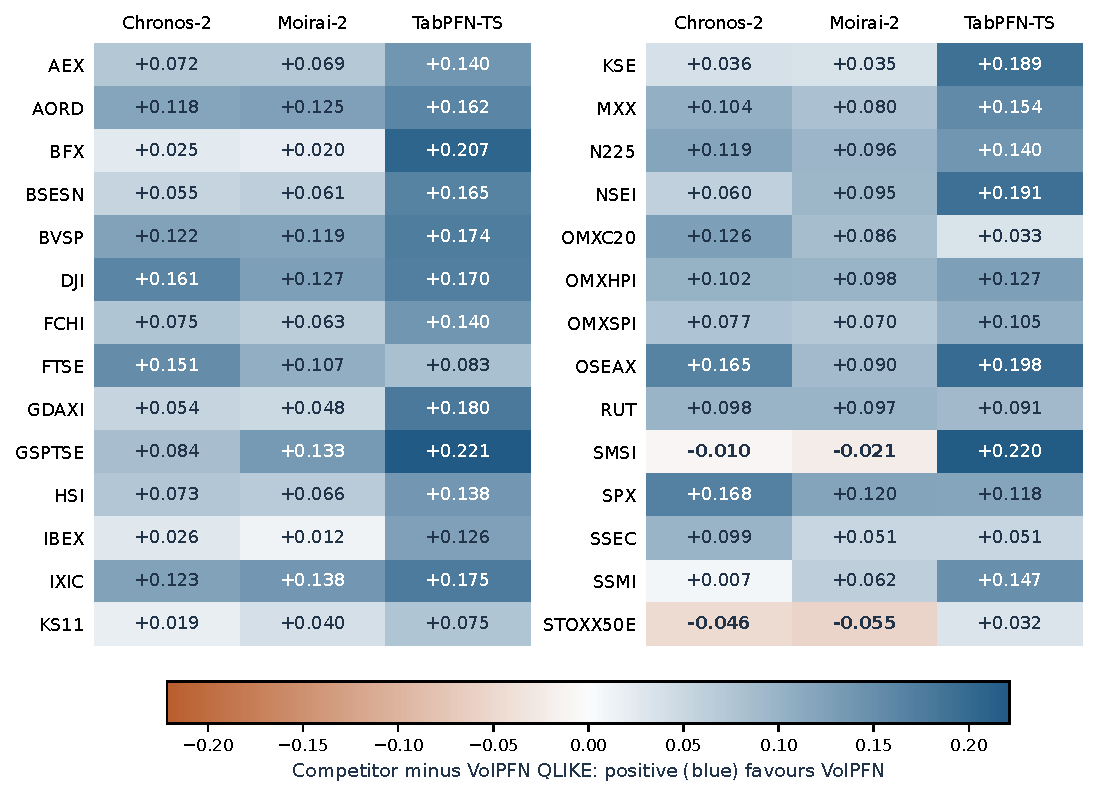
\includegraphics[width=\textwidth]{forecasting_benchmark_markets.pdf}
\caption[Corrected benchmark gains in every market]{Five-model mean competitor-minus-VolPFN QLIKE by market on the same fixed-scale benchmark panel. Blue means lower loss for VolPFN; orange means the competitor performs better. All 28 markets are shown alphabetically in two blocks. Entries are descriptive averages, not separate market-level significance tests.}
\label{fig:benchmark-market-heatmap}
\end{figure}

Historical GARCH-$t$ fits a constant mean, GARCH$(1,1)$ coefficients and tail thickness on the latest 1,000 observations, refits every 250, and updates states between fits. Seven or eight later-period refits occur per market; a failure stops the comparison rather than removing dates. UniVol uses twelve gains, five Student laws and four leverage coefficients, with restart experts favouring recent history. EWMA is initialised before scoring. These schedules are tested choices rather than established optima.

\begin{figure}[!htbp]
\centering
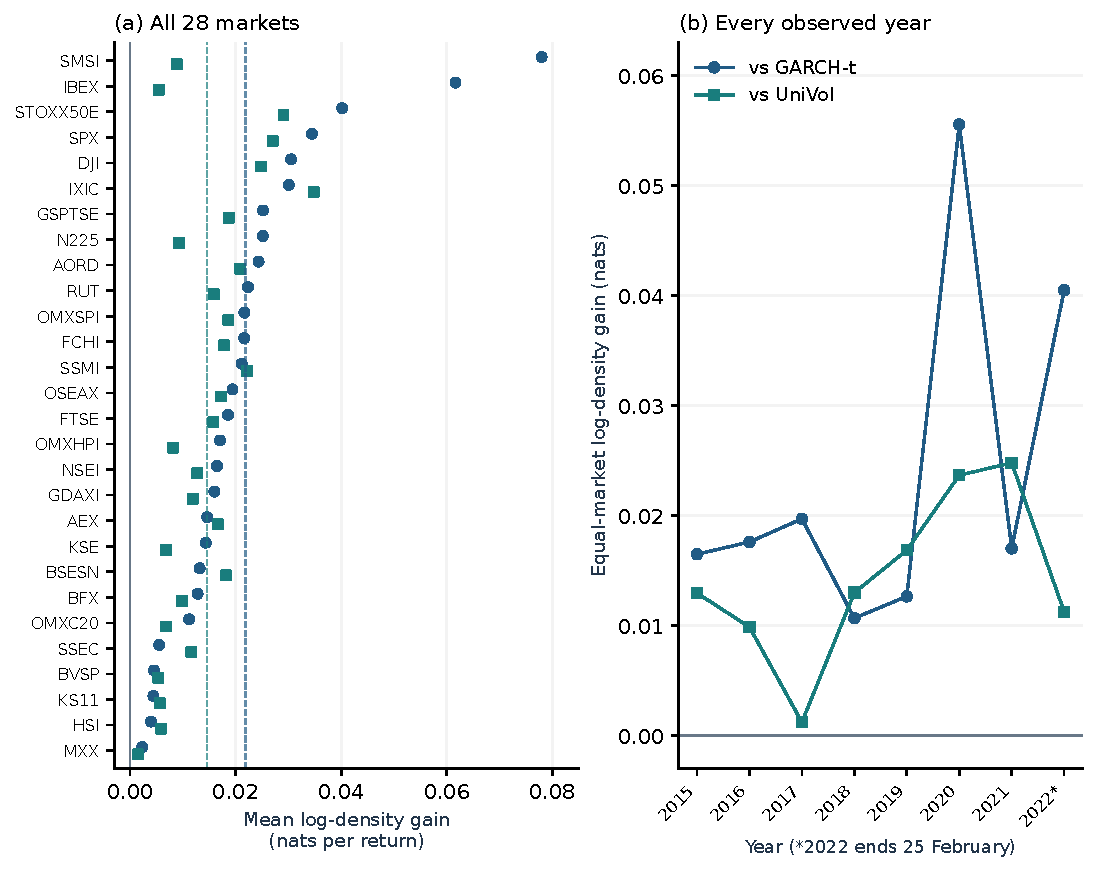
\includegraphics[width=\textwidth]{forecasting_historical_breakdown.pdf}
\caption[Where and when the historical density advantage appears]{Retained-checkpoint native log-density gains, 2015--25 February 2022. Left: all 28 market means, sorted by gain over GARCH-$t$; dashed lines are the two equal-market panel means. Right: every observed calendar year, averaging dates within each market and then markets equally. The partial 2022 period is marked. These descriptive breakdowns use existing scores and introduce no new significance tests.}
\label{fig:historical-breakdown}
\end{figure}

These selected tables complement the complete added-study comparisons in Appendix~\ref{sec:new-research-results}. Each retains its own model identity and statistical family.

\begin{table}[!htbp]\centering
\begingroup\small\setlength{\tabcolsep}{4pt}
\caption[Scores for daily financial neural predictors]{Complete daily neural procedures, 28 markets and 50,073 rows per seed, 2015--February 2022. Five seed losses receive equal weight. Squared-return QLIKE uses second moment; common-$t_8$ NLL fixes shape and native NLL uses the issued density. Lower is better.}\label{tab:new-daily-scores}
\begin{tabular}{@{}lrrr@{}}
\toprule
Procedure & $r^2$ QLIKE & Common-$t_8$ NLL & Native NLL \\
\midrule
Full VolPFN & 0.590700 & 1.184313 & 1.178272 \\
ARCH-LSTM & 0.966913 & 1.349906 & 1.268911 \\
GARCH-LSTM & 0.661074 & 1.217295 & 1.208403 \\
GINN & 0.637127 & 1.205744 & 1.204040 \\
\bottomrule
\end{tabular}\endgroup\end{table}

\begin{table}[!htbp]\centering
\begingroup\small\setlength{\tabcolsep}{4pt}
\caption[Selected common-period daily scores]{Selected raw daily-return procedures on the identical 22,026 keys, 2019--February 2022. Squared-return scoring uses second moment and RK scoring uses central variance. The full 30 September arm is the registered reference. Other daily rows, older versions and ablations remain in Appendix~\ref{sec:new-research-results}; this selection is not a claim of supported superiority over every row.}\label{tab:new-daily-common}
\begin{tabular}{@{}>{\raggedright\arraybackslash}p{6.5cm}rrr@{}}
\toprule
Procedure & $r^2$ QLIKE & RK QLIKE & Seeds \\
\midrule
Full VolPFN (30 September) & 0.703714 & 0.625668 & 5 \\
GJR-GARCH-$t$ & 0.718424 & 0.634702 & 1 \\
APARCH-$t$ & 0.722381 & 0.642651 & 1 \\
GARCH-$t$ & 0.740170 & 0.656740 & 1 \\
GINN & 0.748601 & 0.673846 & 5 \\
UniVol & 0.754697 & 0.681621 & 1 \\
GARCH-LSTM & 0.765202 & 0.710314 & 5 \\
EWMA & 0.770326 & 0.695458 & 1 \\
TabPFN-TS & 0.866181 & 0.760323 & 1 \\
ARCH-LSTM & 1.052799 & 1.021653 & 5 \\
\bottomrule
\end{tabular}\endgroup\end{table}

\begin{table}[!htbp]\centering
\begingroup\small\setlength{\tabcolsep}{4pt}
\caption[Selected realised-risk scores]{Selected realised-risk procedures, 22,026 common keys in 2019--February 2022. These have different information and fitting opportunities. Return-moment inputs use M2 for $r^2$ and variance for RK; native RK procedures use their issued risk level. Proxy-specific blends are fitted separately. GNNHAR's lower mean is included; these descriptive rows do not identify supported superiority.}\label{tab:new-intraday}
\begin{tabular}{@{}>{\raggedright\arraybackslash}p{6.5cm}rrr@{}}
\toprule
Procedure & $r^2$ QLIKE & RK QLIKE & Seeds \\
\midrule
GNNHAR adaptation & 0.669351 & 0.594805 & 5 \\
Full VolPFN+TTM-RK & 0.672139 & 0.598944 & 5 \\
GJR-GARCH-$t$+TTM-RK & 0.675318 & 0.601493 & 1 \\
QLIKE-HAR & 0.678331 & 0.599113 & 1 \\
Transfer-XGBoost & 0.693250 & 0.607646 & 5 \\
TTM-RK & 0.676869 & 0.611457 & 1 \\
Log-HAR & 0.686607 & 0.612740 & 1 \\
MS-HAR & 0.698336 & 0.623273 & 1 \\
Log-Rough-HAR & 0.710735 & 0.656406 & 1 \\
\bottomrule
\end{tabular}\endgroup\end{table}

\FloatBarrier

\section{Supplementary checks of the predictive explanation}
\label{sec:supplementary-analysis}

The supporting studies retain their development, fitting and checkpoint identities. They extend interpretation of compact recovery without providing new confirmation of the five-pair prior experiment.

\subsection{Which part of the short rule matters?}

We keep the asymmetric core fixed while adding horizons, interactions or both. Absolute-level alternatives are measured relative to initial market scale, preventing arbitrary return units from favouring relative-scale terms.

Table~\ref{tab:driver-results} uses $S_t$, the latest squared return divided by predicted risk minus one, and $d_2$, the standardised log difference between the 20- and 100-observation exponential averages. Multiplying them changes shock responsiveness; adding $d_2$ changes risk without needing a large current shock. The comparison examines these attained responses subject to fitting outcomes.

\begin{table}[!htbp]
\centering
\caption[State-variable comparisons]{Selected driver comparisons under likelihood estimation. Differences are common-$t_8$ log scores on the omitted geographical groups. All intervals are conditional development intervals; unequal optimiser convergence prevents an optimised class ordering.}
\label{tab:driver-results}
\small
\begin{tabular}{p{0.47\textwidth}rrr}
\toprule
Candidate minus comparator & Difference & 95\% interval & Markets \\
\midrule
Additive horizon terms minus asymmetric core & $+0.00310$ & $[0.00061,0.00538]$ & 23/28 \\
Shock--horizon interactions minus asymmetric core & $+0.00012$ & $[-0.00076,0.00091]$ & 13/28 \\
Full rule minus asymmetric core & $+0.00325$ & $[0.00082,0.00551]$ & 24/28 \\
$S_td_2$ minus current-scale interaction & $+0.00055$ & $[0.00019,0.00094]$ & 21/28 \\
$S_td_2$ minus long-level interaction & $+0.00040$ & $[0.00005,0.00078]$ & 22/28 \\
\bottomrule
\end{tabular}
\end{table}

The additive horizon rule retains 81.4\% of the network advantage, compared with 52.3\% for interactions and 82.8\% for the full rule. The latter is a different fit from the earlier 82.9\% result. Table~\ref{tab:driver-results} gives a positive conditional interval for direct adjustment and an interval crossing zero for interactions alone. Selected relative-scale fits outperform two absolute-level alternatives under the recorded Holm adjustment, with adjusted tail areas 0.002 and 0.023, but neither reaches the materiality criterion. These selected single-interaction fits converge without establishing global optima.

Unequal optimisation qualifies the recovery comparison. Only 57 of 68 likelihood fits and 45 of 68 path fits converge. Across four geographical likelihood folds, additive-only and asymmetric-core fits all converge, but interaction-only fails in Europe and Asia-Pacific and the full rule fails in Asia-other. Selected single relative-scale and absolute-level interaction fits converge in every fold; the separate three-level absolute interaction fails in all four. Consequently, 81.4\% versus 52.3\% describes attained-budget performance rather than optimised classes. The claim of intrinsic or optimal additive superiority remains withdrawn. The positive additive gain over the converged core still supports useful horizons, while a fair comparison of achievable driver-class performance would require a matched continued refit absent from these scores.



Figure~\ref{fig:compact-components} distinguishes attained recovery from the additive-horizon gain. Appendix~\ref{app:analysis-support} retains further fitting limits, and shock-dependent sensitivity remains possible more generally.


\subsection{Checking the role of the fitting objective}

STES provides an established alternative that uses predictors to change the weight on the latest squared return \citep{taylor2004smooth,ho2022stes}. Horizon information therefore alters responsiveness rather than adding a level adjustment. Our daily-return adaptation uses the latest square, five- and 22-observation averages, and log-level/log-ratio variants; it does not replicate an intraday-realised-variance implementation.

For each market, we fit pre-2011 observations using mean squared error (MSE) or Student likelihood, then evaluate development dates. Mean absolute error (MAE) is another reported measure. This differs from geographical coefficient transfer. Noisy squared returns and alternative losses weight large shocks differently \citep{patton2011volatility}, so failure under one objective cannot establish that an input is unhelpful under every objective.

\begin{table}[!htbp]
\centering
\caption[Smooth-transition smoothing comparisons]{STES comparisons that determine the interpretation. Except for the first row, differences are in common-$t_8$ log density. The first row uses negative absolute error, so positive differences consistently favour the candidate.}
\label{tab:stes-results}
\small
\begin{tabular}{>{\raggedright\arraybackslash}p{0.37\textwidth}>{\raggedright\arraybackslash}p{0.17\textwidth}rr}
\toprule
Candidate minus comparator & Fit; evaluation & Difference & 95\% interval \\
\midrule
Daily/weekly/monthly proxies minus daily square & MSE; $-$MAE & $-0.02411$ & $[-0.03134,-0.01742]$ \\
Daily/weekly/monthly proxies minus daily square & MSE; log score & $-0.02052$ & $[-0.02403,-0.01680]$ \\
Daily/weekly/monthly proxies minus daily square & Likelihood; log score & $+0.00039$ & $[-0.00072,0.00153]$ \\
20/100 log ratio minus daily square & Likelihood; log score & $+0.00315$ & $[0.00110,0.00534]$ \\
20/100 log ratio minus 22-day log level & Likelihood; log score & $+0.00068$ & $[-0.00124,0.00292]$ \\
\bottomrule
\end{tabular}
\end{table}

Likelihood fitting removes the large disadvantage of the daily/weekly/monthly transition set without establishing a positive reversal. The 20/100 ratio improves on the daily-square input in 27 markets, but not conclusively over the 22-day log level, leaving the joint rule unmet. Further development contrasts favour 20/100 over 5/22 by 0.00260 nats, with interval $[0.00044,0.00484]$. Freeing its two log-level coefficients gives $-0.00053$ relative to the ratio, with interval $[-0.00118,0.00010]$. All 1,008 expanded fits converge. These attained comparisons show horizon sensitivity, while successive development tests do not independently confirm a unique ratio mechanism.

\subsection{Supporting evidence from earlier prior restrictions}

The earlier smaller-network study compares broad, random-GARCH and fixed-Gaussian priors with architecture, head, auxiliary weight, lengths, overlays and 6,000 updates shared. Final checkpoints avoid selection on validation mixtures favouring broad training.

Fixing GARCH parameters at $(0.03,0.05,0.92)$ and innovations to Gaussian gives the narrowest prior. It restricts diversity and shock law together while retaining observation modifications, making this another combined-design comparison. The positive control requires broad training to improve on UniVol by 0.005 nats before narrower alternatives are interpreted.

\begin{table}[!htbp]
\centering
\caption[Completed prior-ablation runs]{Completed smaller-network ablations: common-$t_8$ advantage over UniVol, in nats per return. Seed 4 is an additional broad-prior run, not a replacement paired observation for seed 3.}
\label{tab:prior-ablation}
\small
\begin{tabular}{lrrrr}
\toprule
Training prior & Seed 1 & Seed 2 & Seed 3 & Seed 4 \\
\midrule
Broad & $+0.00555$ & $+0.00738$ & Failed & $+0.00604$ \\
Random-parameter GARCH & $-0.00292$ & $-0.00155$ & $-0.00235$ & --- \\
Fixed Gaussian GARCH & $-0.01056$ & $-0.00988$ & $-0.00837$ & --- \\
\bottomrule
\end{tabular}
\end{table}

Completed broad runs pass the control, whereas GARCH-only runs have negative panel advantages. Broad seed 3 fails on a nonfinite simulated return, and seed 4 adds an unpaired run rather than replacing it. Only two genuine broad-versus-narrow pairs remain, with mean gains 0.00870 over random GARCH and 0.01669 over fixed Gaussian. Random-minus-fixed uses three pairs and averages 0.00733. All completed paired differences are positive with individual date intervals excluding zero; those intervals do not include training-seed uncertainty.

These completed pairs favour broader simulation under the smaller budget, while the incomplete battery leaves the base-scale comparison unresolved. A separate output regression finds horizon terms even after fixed-Gaussian training. Preprocessing, architecture, overlays and correlated predictors may produce these terms, preventing their unique attribution to the broad prior. That negative attribution finding remains relevant to the later matched result.



\subsection{Details for interpreting the primary findings}
\label{sec:prior-interpretation-details}

% CLARITY PRECISION TABLE BEGIN
\begin{table}[H]
\centering\small
\caption[Recorded precision for values rounded in prose]{Previously reported values retained at their recorded precision. The scale--shape substitution averages both replacement orders for the earlier checkpoint's development comparison with UniVol. The concentration measure uses the matched prior test, and the recovery denominator uses the original compact study. These values belong to distinct studies; no new calculation is introduced.}
\label{tab:clarity-precision}
\begin{tabular}{lr}
\toprule
Quantity & Recorded value \\
\midrule
Substitution contribution from scale (nats) & 0.00778 \\
Substitution contribution from standardised shape (nats) & 0.00433 \\
Three largest markets' share of net prior gain & 50.6\% \\
Compact recovery denominator (nats) & 0.01025356 \\
\bottomrule
\end{tabular}
\end{table}
% CLARITY PRECISION TABLE END

Single-market omissions give matched-prior gains from 0.00414 to 0.00555 nats; removing the three largest contributors jointly leaves about 0.00301. These are post-result descriptive summaries, without new uncertainty intervals.

The matched prior equivalence interval is $[0.0024642,0.0076740]$, outside the declared $\pm0.003$ band. Its superiority analysis uses 5,000 resamples and 60-date blocks conditional on the ten fitted models. In the separate component programme, historical mean QLIKE is 221.292094 against 0.590118 for synthetic noaux; the gain is 220.701975 with interval $[168.500456,263.777505]$ and adjusted $p=0.000150$. The historical median is about 0.554, and 15,163 of 250,365 seed-level forecasts have QLIKE above 100. The original secondary RK diagnostic uses M2 and differs from the harmonised central-variance score. These original historical losses remain preserved diagnostics; the completed development-selected comparator in Section~\ref{sec:improved-historical} supersedes them as the principal training-source evidence.

The nine-parameter distillation rule's one-step gain over UniVol is 0.00765 nats with interval $[0.00543,0.00979]$; path gain is 0.00652 with interval $[0.00445,0.00861]$. These concern the original compression study, not the expanded driver fits. Convergence does not establish global optimality.

In synthetic tracking, the worst within-window ratio to the numerical reference is 2.14 for sparse settings against a 1.5 threshold, and 1.91 for dense settings against 1.3. The worst sparse ratio to restart experts is 1.17. The proposed sufficiently steep beyond-window deterioration also fails its recorded rule. The earlier rate classification based on goodness-of-fit values for differently transformed responses is withdrawn: such values do not distinguish logarithmic from polynomial growth. The reference uses the known law and initial state with support based on the largest visited state; support checks establish no uniform error bound. The hindsight fixed filter has additional outcome information, and only seven of eighteen simulation-fitted explicit rules converge.
\FloatBarrier

\section{Evidence locations and reproduction}
\label{sec:evidence-locations}

Portable summaries and figure inputs are held in \path{audit/} and \path{research_evidence/}. Full density, compact-rule, tracking and tail records remain in the research archives. The source README and archived unabridged appendices document paths, commands and chronology. Reconstruction from saved losses cannot recover every intermediate forecast or establish that numerical constraints never activate.

\section{Complete results for the added research}
\label{sec:new-research-results}

Each table retains its study's eligibility mask, reference and comparison family. Ordinary intervals, family intervals and seed ranges answer different questions and remain separately labelled.

\subsection{Full-period programme and the failed historical arm}

\begin{table}[H]\centering
\begingroup\small\setlength{\tabcolsep}{4pt}
\caption[All training-configuration scores]{All seven programme arms on the full 2015--February 2022 population. The secondary RK score uses second moment and its own 50,054-row-per-seed mask; it must not be substituted for the later central-variance RK score. Direct has no native density. Lower losses are preferred.}\label{tab:new-all-programme}
\begin{tabular}{@{}>{\raggedright\arraybackslash}p{3.3cm}rrrr@{}}
\toprule
Procedure & $r^2$ QLIKE & Common $t_8$ & Native NLL & RK (M2) \\
\midrule
Full VolPFN & 0.590700 & 1.184313 & 1.178272 & 0.511232 \\
Noaux & 0.590118 & 1.183908 & 1.177252 & 0.510703 \\
Direct second moment & 0.599658 & 1.188399 & --- & 0.512668 \\
Historical training & 221.292094 & 2.893771 & 33.109706 & 194.478753 \\
ARCH-LSTM & 0.966913 & 1.349906 & 1.268911 & 0.930030 \\
GARCH-LSTM & 0.661074 & 1.217295 & 1.208403 & 0.600828 \\
GINN & 0.637127 & 1.205744 & 1.204040 & 0.556977 \\
\bottomrule
\end{tabular}\endgroup\end{table}

\begin{table}[H]\centering
\begingroup\footnotesize\setlength{\tabcolsep}{3pt}
\caption[Training-component gains by seed]{Individual programme seeds: equal-market squared-return QLIKE on the complete 2015--February 2022 population. Rows are separate models, not ensembles.}\label{tab:new-programme-seeds}
\begin{tabular}{@{}lrrrrrrr@{}}
\toprule
Seed & Full & Noaux & Direct & Historical & ARCH-LSTM & GARCH-LSTM & GINN \\
\midrule
8101 & 0.591322 & 0.590379 & 0.601184 & 175.556160 & 0.965816 & 0.649599 & 0.637093 \\
8102 & 0.590656 & 0.587933 & 0.597818 & 201.027320 & 0.969667 & 0.671457 & 0.635955 \\
8103 & 0.589893 & 0.590018 & 0.604661 & 241.386418 & 0.964629 & 0.651213 & 0.642117 \\
8104 & 0.591311 & 0.590699 & 0.598014 & 297.314084 & 0.965232 & 0.659670 & 0.632799 \\
8105 & 0.590316 & 0.591563 & 0.596613 & 191.176486 & 0.969221 & 0.673432 & 0.637670 \\
\bottomrule
\end{tabular}\endgroup\end{table}

\begingroup\footnotesize\setlength{\tabcolsep}{3pt}
\begin{longtable}{@{}lrrrrrrr@{}}
\caption[Training-component gains by market]{Market means for the component and dedicated daily study, 2015--February 2022. Values average five seed losses within each market. Unequal record lengths do not weight the panel mean. The large historical losses are retained.}\label{tab:new-programme-markets}\\
\toprule
Market & Full & Noaux & Direct & Historical & ARCH & GARCH & GINN \\
\midrule\endfirsthead
\toprule
Market & Full & Noaux & Direct & Historical & ARCH & GARCH & GINN \\
\midrule\endhead
AEX & 0.307995 & 0.306063 & 0.322902 & 224.895262 & 0.736341 & 0.369218 & 0.361762 \\
AORD & 0.505451 & 0.504763 & 0.515767 & 194.176219 & 0.671421 & 0.526023 & 0.535050 \\
BFX & 0.415439 & 0.415061 & 0.418987 & 555.574760 & 0.681943 & 0.440432 & 0.459312 \\
BSESN & 0.595804 & 0.596475 & 0.609197 & 76.669727 & 1.034018 & 0.692721 & 0.629544 \\
BVSP & 0.981502 & 0.983121 & 0.985838 & 226.666016 & 1.333499 & 1.061347 & 1.040994 \\
DJI & 0.261692 & 0.260164 & 0.274401 & 177.602068 & 0.807717 & 0.378182 & 0.358568 \\
FCHI & 0.500187 & 0.497901 & 0.514031 & 581.534543 & 0.863135 & 0.554966 & 0.556809 \\
FTSE & 0.731466 & 0.731983 & 0.746558 & 139.500838 & 1.020572 & 0.774449 & 0.781394 \\
GDAXI & 0.695488 & 0.693904 & 0.715287 & 126.800414 & 1.035813 & 0.751182 & 0.748027 \\
GSPTSE & -0.216739 & -0.217893 & -0.206891 & 192.013638 & 0.378635 & -0.035425 & -0.117972 \\
HSI & 0.650265 & 0.651581 & 0.650462 & 160.671346 & 0.812766 & 0.668526 & 0.672647 \\
IBEX & 0.687386 & 0.685351 & 0.687539 & 299.716951 & 1.028851 & 0.713983 & 0.712204 \\
IXIC & 0.653567 & 0.653139 & 0.669081 & 336.419421 & 1.170668 & 0.739529 & 0.717200 \\
KS11 & 0.200748 & 0.202232 & 0.201809 & 202.451337 & 0.805178 & 0.350308 & 0.245721 \\
KSE & 0.810501 & 0.807684 & 0.818471 & 136.702667 & 1.119874 & 0.870487 & 0.851475 \\
MXX & 0.628318 & 0.628994 & 0.628110 & 175.026482 & 1.023769 & 0.680181 & 0.633288 \\
N225 & 0.530539 & 0.531215 & 0.536371 & 199.611627 & 0.884572 & 0.623965 & 0.598585 \\
NSEI & 0.558244 & 0.557847 & 0.578476 & 245.116532 & 0.876870 & 0.587450 & 0.585291 \\
OMXC20 & 0.991254 & 0.989308 & 1.003431 & 189.654288 & 1.181254 & 1.017881 & 1.013313 \\
OMXHPI & 0.491254 & 0.491342 & 0.502571 & 165.768945 & 1.053381 & 0.641089 & 0.557585 \\
OMXSPI & 0.438294 & 0.436547 & 0.447499 & 180.050416 & 1.085286 & 0.586040 & 0.482323 \\
OSEAX & 0.920134 & 0.918636 & 0.941834 & 160.015300 & 1.179178 & 0.994276 & 0.972340 \\
RUT & 0.993527 & 0.994288 & 1.002787 & 170.932093 & 1.169371 & 1.024047 & 1.012883 \\
SMSI & 0.822091 & 0.820251 & 0.816680 & 205.204763 & 1.076206 & 0.843808 & 0.846751 \\
SPX & 0.223903 & 0.223274 & 0.238277 & 222.671830 & 0.804136 & 0.342858 & 0.340832 \\
SSEC & 0.994067 & 0.994996 & 0.989708 & 191.561889 & 1.413150 & 1.060551 & 1.004844 \\
SSMI & 0.365734 & 0.365701 & 0.359111 & 161.854790 & 0.620202 & 0.384701 & 0.369079 \\
STOXX50E & 0.801475 & 0.799389 & 0.822131 & 297.314457 & 1.205750 & 0.867301 & 0.869703 \\
\bottomrule
\end{longtable}\endgroup


We average scores across dates within each market, then give markets and seeds equal weight. Each seed is scored separately; the forecasts are not ensembled. The original fixed-final historical arm remains as a diagnostic; Section~\ref{sec:improved-historical} supplies the stronger completed comparator and Appendix~\ref{sec:followup-results} its separate inference. Maximum QLIKE is about 3.72 million and minimum issued second moment about $1.09\times10^{-6}$. All four configurations share one-position extrapolation: the largest trained prediction position is 1022, while evaluation reaches 1023. Neither pinned replay nor these diagnostics establish a sole failure cause.

\subsection{Common-period daily evidence}

\begingroup\small\setlength{\tabcolsep}{4pt}
\begin{longtable}{@{}>{\raggedright\arraybackslash}p{6.5cm}rrr@{}}
\caption[Complete common-period daily scores]{Complete saved daily table and supplementary configurations, 22,026 keys in 2019--February 2022. The 26 September model and ablations retain distinct identities. RK scoring uses central variance; direct RK is unavailable. Descriptive loss ordering does not transfer tests between model versions.}\label{tab:new-daily-common-all}\\
\toprule
Procedure & $r^2$ QLIKE & RK QLIKE & Seeds \\
\midrule\endfirsthead
\toprule
Procedure & $r^2$ QLIKE & RK QLIKE & Seeds \\
\midrule\endhead
VolPFN (26 September) & 0.703689 & 0.625397 & 5 \\
Full VolPFN (30 September) & 0.703714 & 0.625668 & 5 \\
GJR-GARCH-$t$ & 0.718424 & 0.634702 & 1 \\
APARCH-$t$ & 0.722381 & 0.642651 & 1 \\
GARCH-$t$ & 0.740170 & 0.656740 & 1 \\
GINN & 0.748601 & 0.673846 & 5 \\
UniVol & 0.754697 & 0.681621 & 1 \\
GARCH-LSTM & 0.765202 & 0.710314 & 5 \\
EWMA & 0.770326 & 0.695458 & 1 \\
TabPFN-TS & 0.866181 & 0.760323 & 1 \\
ARCH-LSTM & 1.052799 & 1.021653 & 5 \\
Historical variance (250) & 1.072036 & 1.076967 & 1 \\
EGARCH-$t$ & 2.376730 & 2.303764 & 1 \\
Chronos-2 & 2.478397 & 2.191879 & 1 \\
Moirai-2 & $7.03773\times10^{5}$ & $1.30930\times10^{6}$ & 1 \\
TTM square-root RK diagnostic & 0.687005 & 0.607298 & 1 \\
Noaux & 0.702624 & 0.624696 & 5 \\
Compact nine-parameter rule & 0.705530 & 0.642068 & 1 \\
Direct second moment & 0.712596 & --- & 5 \\
Mean-log HAR diagnostic & 0.713198 & 0.663236 & 1 \\
Historical training & 222.674179 & $1.92096\times10^{4}$ & 5 \\
\bottomrule
\end{longtable}\endgroup

\begingroup\footnotesize\setlength{\tabcolsep}{2pt}
\begin{longtable}{@{}>{\raggedright\arraybackslash}p{2.0cm}lrccr@{}}
\caption[Complete common-period daily inference]{All primary-block contrasts in the separate 28-slot daily family, full 30 September reference. Gains are comparator minus reference. Ordinary and Bonferroni family intervals are distinct; joint support also requires both proxies and all reference-seed directions.}\label{tab:new-daily-inference}\\
\toprule
Comparator & Proxy & Gain & Ordinary 95\% & Family 95\% & Holm $p$ \\
\midrule\endfirsthead
\toprule
Comparator & Proxy & Gain & Ordinary 95\% & Family 95\% & Holm $p$ \\
\midrule\endhead
VolPFN (26 September) & $r^2$ & -0.000025 & $[-0.000511,0.000456]$ & $[-0.000806,0.000699]$ & 0.922604 \\
VolPFN (26 September) & RK & -0.000271 & $[-0.000614,0.000056]$ & $[-0.000841,0.000228]$ & 0.644468 \\
GJR-GARCH-$t$ & $r^2$ & 0.014710 & $[0.002690,0.025596]$ & $[-0.005585,0.030755]$ & 0.185241 \\
GJR-GARCH-$t$ & RK & 0.009034 & $[0.000203,0.016813]$ & $[-0.005703,0.020749]$ & 0.395980 \\
APARCH-$t$ & $r^2$ & 0.018667 & $[-0.007799,0.036714]$ & $[-0.028895,0.041415]$ & 0.644468 \\
APARCH-$t$ & RK & 0.016983 & $[-0.009022,0.033151]$ & $[-0.030504,0.037170]$ & 0.644468 \\
GARCH-$t$ & $r^2$ & 0.036456 & $[0.002342,0.060043]$ & $[-0.025383,0.066577]$ & 0.245038 \\
GARCH-$t$ & RK & 0.031072 & $[-0.003685,0.052449]$ & $[-0.031830,0.056857]$ & 0.447678 \\
GINN & $r^2$ & 0.044887 & $[0.021849,0.066686]$ & $[0.007220,0.079608]$ & 0.002000 \\
GINN & RK & 0.048178 & $[0.020320,0.067348]$ & $[-0.001748,0.073965]$ & 0.020399 \\
UniVol & $r^2$ & 0.050984 & $[0.031216,0.067877]$ & $[0.018917,0.076424]$ & 0.001400 \\
UniVol & RK & 0.055953 & $[0.033186,0.073476]$ & $[0.017825,0.080113]$ & 0.002000 \\
GARCH-LSTM & $r^2$ & 0.061488 & $[0.038481,0.085014]$ & $[0.023466,0.099624]$ & 0.001400 \\
GARCH-LSTM & RK & 0.084646 & $[0.062228,0.105809]$ & $[0.048995,0.117452]$ & 0.001400 \\
EWMA & $r^2$ & 0.066612 & $[0.011440,0.106244]$ & $[-0.031369,0.121346]$ & 0.184791 \\
EWMA & RK & 0.069790 & $[0.008943,0.110205]$ & $[-0.035559,0.119373]$ & 0.200190 \\
TabPFN-TS & $r^2$ & 0.162467 & $[0.127795,0.191350]$ & $[0.103711,0.203598]$ & 0.001400 \\
TabPFN-TS & RK & 0.134655 & $[0.112725,0.154649]$ & $[0.098722,0.164135]$ & 0.001400 \\
ARCH-LSTM & $r^2$ & 0.349085 & $[0.252951,0.448091]$ & $[0.195952,0.508750]$ & 0.001400 \\
ARCH-LSTM & RK & 0.395985 & $[0.295073,0.492363]$ & $[0.240872,0.547212]$ & 0.001400 \\
Historical variance (250) & $r^2$ & 0.368323 & $[-0.115800,0.635827]$ & $[-0.541047,0.668407]$ & 0.644468 \\
Historical variance (250) & RK & 0.451299 & $[-0.167356,0.780805]$ & $[-0.698921,0.809609]$ & 0.644468 \\
EGARCH-$t$ & $r^2$ & 1.673016 & $[-0.833468,3.312847]$ & $[-2.614018,3.345017]$ & 0.644468 \\
EGARCH-$t$ & RK & 1.678096 & $[-0.828472,3.319278]$ & $[-2.613402,3.351321]$ & 0.644468 \\
Chronos-2 & $r^2$ & 1.774683 & $[1.019284,2.293604]$ & $[0.413181,2.430903]$ & 0.001400 \\
Chronos-2 & RK & 1.566211 & $[0.819291,2.035569]$ & $[0.184280,2.137435]$ & 0.002700 \\
Moirai-2 & $r^2$ & $7.03772\times10^{5}$ & $[-7.18415\times10^{5},1.40754\times10^{6}]$ & $[-1.94660\times10^{6},1.40754\times10^{6}]$ & 0.644468 \\
Moirai-2 & RK & $1.30930\times10^{6}$ & $[-1.33241\times10^{6},2.61859\times10^{6}]$ & $[-3.78065\times10^{6},2.61859\times10^{6}]$ & 0.644468 \\
\bottomrule
\end{longtable}\endgroup


Direct predicts second moment without a separately identified central variance. Its earlier M2/RK diagnostic therefore cannot fill the harmonised variance/RK slot. Alignment uses saved forecasts without retraining or calibration. Extreme losses describe the issued procedures rather than all members of a model family.

\subsection{Complete realised-risk and helper comparisons}

\begingroup\small\setlength{\tabcolsep}{4pt}
\begin{longtable}{@{}>{\raggedright\arraybackslash}p{6.5cm}rrr@{}}
\caption[Complete realised-risk scores]{All eighteen completed intraday-extension procedures on the common 2019--February 2022 panel. Lower is better; complete-procedure comparisons do not isolate architecture. Unavailable M2VN and DeepRGARCH retain statistical slots without fabricated scores.}\label{tab:new-intraday-all}\\
\toprule
Procedure & $r^2$ QLIKE & RK QLIKE & Seeds \\
\midrule\endfirsthead
\toprule
Procedure & $r^2$ QLIKE & RK QLIKE & Seeds \\
\midrule\endhead
Full VolPFN+TTM-RK & 0.672139 & 0.598944 & 5 \\
VolPFN (26 Sept.)+TTM-RK & 0.672203 & 0.598948 & 5 \\
Full VolPFN+Log-HAR & 0.675699 & 0.605183 & 5 \\
Full VolPFN+MS-HAR & 0.682335 & 0.609285 & 5 \\
GJR-GARCH-$t$+TTM-RK & 0.675318 & 0.601493 & 1 \\
GJR-GARCH-$t$+Log-HAR & 0.679109 & 0.607935 & 1 \\
MS-HAR+Log-HAR & 0.684291 & 0.615649 & 1 \\
Full VolPFN (30 September) & 0.703714 & 0.625668 & 5 \\
VolPFN (26 September) & 0.703689 & 0.625397 & 5 \\
GJR-GARCH-$t$ & 0.718424 & 0.634702 & 1 \\
HAR & 28.898514 & 31.530660 & 1 \\
Log-HAR & 0.686607 & 0.612740 & 1 \\
TTM-RK & 0.676869 & 0.611457 & 1 \\
MS-HAR & 0.698336 & 0.623273 & 1 \\
Log-Rough-HAR & 0.710735 & 0.656406 & 1 \\
GNNHAR adaptation & 0.669351 & 0.594805 & 5 \\
QLIKE-HAR & 0.678331 & 0.599113 & 1 \\
Transfer-XGBoost & 0.693250 & 0.607646 & 5 \\
\bottomrule
\end{longtable}\endgroup

\begingroup\footnotesize\setlength{\tabcolsep}{3pt}
\begin{longtable}{@{}>{\raggedright\arraybackslash}p{2.7cm}lrccr@{}}
\caption[Complete realised-risk inference]{All primary-block contrasts in the 38-slot intraday family, full VolPFN+TTM reference. Unavailable entries retain $p=1$. Ordinary and Bonferroni family intervals are shown separately. Joint support requires both proxies and all reference-seed directions.}\label{tab:new-intraday-inference}\\
\toprule
Comparator & Proxy & Gain & Ordinary 95\% & Family 95\% & Holm $p$ \\
\midrule\endfirsthead
\toprule
Comparator & Proxy & Gain & Ordinary 95\% & Family 95\% & Holm $p$ \\
\midrule\endhead
VolPFN (26 Sept.)+TTM-RK & $r^2$ & 0.000064 & $[-0.000097,0.000217]$ & $[-0.000198,0.000309]$ & 1.000000 \\
VolPFN (26 Sept.)+TTM-RK & RK & 0.000004 & $[-0.000124,0.000120]$ & $[-0.000208,0.000183]$ & 1.000000 \\
Full VolPFN+Log-HAR & $r^2$ & 0.003560 & $[-0.005272,0.011764]$ & $[-0.011053,0.016594]$ & 1.000000 \\
Full VolPFN+Log-HAR & RK & 0.006240 & $[-0.009361,0.016293]$ & $[-0.023389,0.019753]$ & 1.000000 \\
Full VolPFN+MS-HAR & $r^2$ & 0.010196 & $[-0.005476,0.022851]$ & $[-0.016592,0.029472]$ & 1.000000 \\
Full VolPFN+MS-HAR & RK & 0.010341 & $[-0.009719,0.022438]$ & $[-0.028138,0.025980]$ & 1.000000 \\
GJR-GARCH-$t$+TTM-RK & $r^2$ & 0.003178 & $[0.001303,0.004841]$ & $[-0.000110,0.005768]$ & 0.033598 \\
GJR-GARCH-$t$+TTM-RK & RK & 0.002549 & $[0.000988,0.003926]$ & $[-0.000122,0.004627]$ & 0.034098 \\
GJR-GARCH-$t$+Log-HAR & $r^2$ & 0.006970 & $[-0.004819,0.016608]$ & $[-0.013898,0.021992]$ & 1.000000 \\
GJR-GARCH-$t$+Log-HAR & RK & 0.008991 & $[-0.008927,0.020107]$ & $[-0.024760,0.023645]$ & 1.000000 \\
MS-HAR+Log-HAR & $r^2$ & 0.012152 & $[-0.008476,0.026574]$ & $[-0.026187,0.031898]$ & 1.000000 \\
MS-HAR+Log-HAR & RK & 0.016705 & $[-0.011499,0.033236]$ & $[-0.037620,0.036888]$ & 1.000000 \\
Full VolPFN (30 September) & $r^2$ & 0.031574 & $[0.017986,0.043996]$ & $[0.009333,0.050936]$ & 0.001900 \\
Full VolPFN (30 September) & RK & 0.026724 & $[0.020980,0.032708]$ & $[0.017644,0.036689]$ & 0.001900 \\
VolPFN (26 September) & $r^2$ & 0.031549 & $[0.017971,0.044010]$ & $[0.009263,0.050998]$ & 0.001900 \\
VolPFN (26 September) & RK & 0.026453 & $[0.020694,0.032420]$ & $[0.017357,0.036489]$ & 0.001900 \\
GJR-GARCH-$t$ & $r^2$ & 0.046284 & $[0.023908,0.066211]$ & $[0.008443,0.075818]$ & 0.001900 \\
GJR-GARCH-$t$ & RK & 0.035758 & $[0.025420,0.045467]$ & $[0.018580,0.051432]$ & 0.001900 \\
HAR & $r^2$ & 28.226375 & $[-29.377519,56.447931]$ & $[-85.062870,56.459737]$ & 1.000000 \\
HAR & RK & 30.931716 & $[-32.218364,61.854624]$ & $[-92.823133,61.860491]$ & 1.000000 \\
Log-HAR & $r^2$ & 0.014468 & $[-0.006438,0.032055]$ & $[-0.021355,0.041210]$ & 1.000000 \\
Log-HAR & RK & 0.013796 & $[-0.008934,0.028376]$ & $[-0.028989,0.033451]$ & 1.000000 \\
TTM-RK & $r^2$ & 0.004730 & $[-0.000936,0.010178]$ & $[-0.004558,0.013468]$ & 1.000000 \\
TTM-RK & RK & 0.012513 & $[0.003683,0.021801]$ & $[-0.001702,0.027669]$ & 0.173991 \\
MS-HAR & $r^2$ & 0.026197 & $[-0.003996,0.049557]$ & $[-0.027159,0.060511]$ & 1.000000 \\
MS-HAR & RK & 0.024329 & $[-0.000089,0.039808]$ & $[-0.021841,0.044643]$ & 0.684416 \\
Log-Rough-HAR & $r^2$ & 0.038596 & $[-0.036928,0.083934]$ & $[-0.103821,0.095360]$ & 1.000000 \\
Log-Rough-HAR & RK & 0.057462 & $[-0.054158,0.116379]$ & $[-0.161461,0.121709]$ & 1.000000 \\
GNNHAR adaptation & $r^2$ & -0.002788 & $[-0.017395,0.015490]$ & $[-0.024113,0.027691]$ & 1.000000 \\
GNNHAR adaptation & RK & -0.004139 & $[-0.016860,0.015021]$ & $[-0.020967,0.029546]$ & 1.000000 \\
QLIKE-HAR & $r^2$ & 0.006192 & $[-0.009076,0.022959]$ & $[-0.016646,0.032510]$ & 1.000000 \\
QLIKE-HAR & RK & 0.000170 & $[-0.011345,0.015936]$ & $[-0.015565,0.028032]$ & 1.000000 \\
Transfer-XGBoost & $r^2$ & 0.021110 & $[0.006779,0.035218]$ & $[-0.001801,0.044420]$ & 0.104995 \\
Transfer-XGBoost & RK & 0.008702 & $[0.002141,0.015354]$ & $[-0.001859,0.019703]$ & 0.282786 \\
M2VN (unavailable) & $r^2$ & --- & --- & --- & 1.000000 \\
M2VN (unavailable) & RK & --- & --- & --- & 1.000000 \\
DeepRGARCH (unavailable) & $r^2$ & --- & --- & --- & 1.000000 \\
DeepRGARCH (unavailable) & RK & --- & --- & --- & 1.000000 \\
\bottomrule
\end{longtable}\endgroup

\begin{table}[H]\centering
\begingroup\small\setlength{\tabcolsep}{4pt}
\caption[Complete cross-market-helper scores]{Cross-market-helper follow-up and preserved controls on the same 22,026 keys. All helper-containing procedures score five seed losses separately. The reference is VolPFN+helper, and no comparator passes the separate twelve-slot two-proxy rule.}\label{tab:new-helper-all}
\begin{tabular}{@{}>{\raggedright\arraybackslash}p{6.5cm}rrr@{}}
\toprule
Procedure & $r^2$ QLIKE & RK QLIKE & Seeds \\
\midrule
GNNHAR adaptation & 0.669351 & 0.594805 & 5 \\
Full VolPFN+TTM-RK & 0.672139 & 0.598944 & 5 \\
VolPFN+helper & 0.674026 & 0.603577 & 5 \\
GJR+helper & 0.677955 & 0.606815 & 5 \\
Transfer-XGBoost & 0.693250 & 0.607646 & 5 \\
Cross-market helper & 0.686927 & 0.618399 & 5 \\
Calibrated helper & 0.694879 & 0.644218 & 5 \\
\bottomrule
\end{tabular}\endgroup\end{table}

\begingroup\footnotesize\setlength{\tabcolsep}{3pt}
\begin{longtable}{@{}>{\raggedright\arraybackslash}p{2.7cm}lrccr@{}}
\caption[Cross-market-helper inference]{All primary-block contrasts in the separate twelve-slot helper family, VolPFN+helper reference. Ordinary and family intervals are distinct. Joint support requires both proxies and corresponding seed directions; no contrast meets the complete rule.}\label{tab:new-helper-inference}\\
\toprule
Comparator & Proxy & Gain & Ordinary 95\% & Family 95\% & Holm $p$ \\
\midrule\endfirsthead
\toprule
Comparator & Proxy & Gain & Ordinary 95\% & Family 95\% & Holm $p$ \\
\midrule\endhead
Calibrated helper & $r^2$ & 0.020853 & $[-0.000781,0.034324]$ & $[-0.014486,0.037312]$ & 0.207540 \\
Calibrated helper & RK & 0.040641 & $[-0.011515,0.068908]$ & $[-0.051015,0.071198]$ & 0.419679 \\
GJR+helper & $r^2$ & 0.003929 & $[0.000753,0.006443]$ & $[-0.001145,0.007410]$ & 0.093595 \\
GJR+helper & RK & 0.003238 & $[0.001269,0.004910]$ & $[0.000142,0.005580]$ & 0.019799 \\
Cross-market helper & $r^2$ & 0.012900 & $[0.004429,0.020533]$ & $[0.000455,0.023670]$ & 0.020349 \\
Cross-market helper & RK & 0.014822 & $[0.005537,0.021121]$ & $[-0.000029,0.023125]$ & 0.021499 \\
Full VolPFN+TTM-RK & $r^2$ & -0.001887 & $[-0.010294,0.006141]$ & $[-0.013763,0.009722]$ & 1.000000 \\
Full VolPFN+TTM-RK & RK & -0.004634 & $[-0.010436,0.002143]$ & $[-0.012897,0.005651]$ & 0.712464 \\
GNNHAR adaptation & $r^2$ & -0.004675 & $[-0.016137,0.008789]$ & $[-0.020064,0.016260]$ & 1.000000 \\
GNNHAR adaptation & RK & -0.008772 & $[-0.022388,0.014764]$ & $[-0.025260,0.029053]$ & 1.000000 \\
Transfer-XGBoost & $r^2$ & 0.019223 & $[0.002313,0.033344]$ & $[-0.006677,0.038430]$ & 0.130793 \\
Transfer-XGBoost & RK & 0.004068 & $[-0.003265,0.012671]$ & $[-0.006041,0.017110]$ & 1.000000 \\
\bottomrule
\end{longtable}\endgroup

\clearpage
\begin{table}[!htbp]\centering
\begingroup\small\setlength{\tabcolsep}{4pt}
\caption[Common-period reference seeds]{Equal-market descriptive seed losses on the same 22,026 keys. These are separately scored forecasts, not ensembles or independent significance tests.}\label{tab:new-common-seeds}
\begin{tabular}{@{}l>{\raggedright\arraybackslash}p{6cm}rr@{}}
\toprule
Seed & Procedure & $r^2$ QLIKE & RK QLIKE \\
\midrule
8101 & Full VolPFN+TTM-RK & 0.672112 & 0.598389 \\
8101 & GNNHAR adaptation & 0.669137 & 0.595102 \\
8101 & VolPFN+helper & 0.675812 & 0.603673 \\
8102 & Full VolPFN+TTM-RK & 0.672698 & 0.600277 \\
8102 & GNNHAR adaptation & 0.670172 & 0.594903 \\
8102 & VolPFN+helper & 0.673559 & 0.604507 \\
8103 & Full VolPFN+TTM-RK & 0.671690 & 0.598390 \\
8103 & GNNHAR adaptation & 0.670782 & 0.595442 \\
8103 & VolPFN+helper & 0.672844 & 0.602767 \\
8104 & Full VolPFN+TTM-RK & 0.672015 & 0.598924 \\
8104 & GNNHAR adaptation & 0.667610 & 0.594185 \\
8104 & VolPFN+helper & 0.674199 & 0.603934 \\
8105 & Full VolPFN+TTM-RK & 0.672181 & 0.598739 \\
8105 & GNNHAR adaptation & 0.669054 & 0.594394 \\
8105 & VolPFN+helper & 0.673718 & 0.603006 \\
\bottomrule
\end{tabular}\endgroup\end{table}

\clearpage
\begingroup\footnotesize\setlength{\tabcolsep}{3pt}
\begin{longtable}{@{}lrrrrrr@{}}
\caption[Realised-risk gains by market]{Descriptive market gains relative to VolPFN+TTM on common keys. Five seed losses are averaged where available; GJR+TTM is a single deterministic procedure. Positive favours the reference. GNN denotes GNNHAR, GJR denotes GJR+TTM and Transfer denotes Transfer-XGBoost. These market means are not separate adjusted tests.}\label{tab:new-intraday-markets}\\
\toprule
Market & GNN $r^2$ & GNN RK & GJR $r^2$ & GJR RK & Transfer $r^2$ & Transfer RK \\
\midrule\endfirsthead
\toprule
Market & GNN $r^2$ & GNN RK & GJR $r^2$ & GJR RK & Transfer $r^2$ & Transfer RK \\
\midrule\endhead
AEX & -0.004880 & 0.003499 & 0.004816 & 0.001219 & 0.005588 & 0.010200 \\
AORD & 0.011702 & -0.000012 & 0.004369 & 0.004830 & 0.026337 & 0.016252 \\
BFX & -0.028661 & -0.019229 & 0.000518 & -0.000531 & -0.020708 & -0.001484 \\
BSESN & 0.009606 & -0.006744 & 0.003066 & 0.004445 & 0.035817 & 0.006712 \\
BVSP & -0.008100 & -0.017983 & -0.002132 & -0.002900 & 0.000882 & -0.004826 \\
DJI & -0.016879 & -0.004871 & 0.001964 & 0.002608 & 0.024665 & 0.015848 \\
FCHI & -0.022963 & -0.006115 & 0.003307 & 0.000874 & -0.016859 & 0.006464 \\
FTSE & -0.026164 & -0.000944 & 0.004177 & -0.000496 & 0.011362 & 0.006281 \\
GDAXI & 0.020021 & -0.006141 & 0.005131 & 0.002833 & 0.041264 & 0.002598 \\
GSPTSE & -0.020960 & -0.000810 & 0.011588 & 0.005500 & 0.032637 & 0.024393 \\
HSI & 0.003172 & -0.010581 & 0.001861 & 0.004211 & 0.017058 & 0.000031 \\
IBEX & -0.002851 & -0.001081 & 0.005330 & 0.008744 & -0.006339 & 0.008881 \\
IXIC & -0.016576 & -0.003281 & -0.002364 & -0.000847 & 0.009439 & 0.015606 \\
KS11 & -0.019007 & 0.001445 & 0.006160 & 0.005431 & 0.010241 & 0.016196 \\
KSE & 0.014723 & -0.016338 & 0.002176 & 0.003037 & 0.041852 & -0.001262 \\
MXX & 0.019970 & -0.003170 & -0.000021 & 0.000261 & 0.030215 & 0.005832 \\
N225 & 0.003498 & -0.006222 & 0.000305 & -0.000808 & 0.029530 & 0.002777 \\
NSEI & 0.021473 & -0.003104 & 0.001778 & 0.000890 & 0.071996 & 0.019171 \\
OMXC20 & 0.011535 & -0.009548 & 0.001636 & 0.001347 & 0.025091 & -0.002972 \\
OMXHPI & 0.007281 & -0.000893 & 0.007049 & 0.003464 & 0.021098 & 0.014014 \\
OMXSPI & 0.004083 & 0.005850 & 0.003951 & 0.002451 & 0.018173 & 0.016870 \\
OSEAX & 0.009113 & -0.011555 & 0.008399 & 0.007868 & 0.036921 & -0.001453 \\
RUT & 0.004147 & 0.008881 & 0.003160 & 0.005286 & 0.033490 & 0.021941 \\
SMSI & -0.009324 & 0.008057 & -0.001772 & 0.001369 & 0.004097 & 0.009261 \\
SPX & -0.021135 & -0.001771 & 0.001413 & 0.002497 & 0.019871 & 0.017648 \\
SSEC & 0.018688 & -0.006713 & 0.001787 & 0.001090 & 0.048157 & -0.003318 \\
SSMI & -0.035504 & -0.016728 & 0.004288 & 0.004047 & -0.004587 & -0.004951 \\
STOXX50E & -0.004078 & 0.010216 & 0.007051 & 0.002662 & 0.043803 & 0.026951 \\
\bottomrule
\end{longtable}\endgroup


Both proxies must satisfy the complete registered joint rule for support. Market signs and seed ranges remain descriptive. The bundle retains block-20/120 sensitivities and complete seed and market records; inference conditions on saved forecasts without training or refitting uncertainty.

\subsection{Unavailable procedures, failures and remaining experiments}

Unavailable procedures remain visible: M2VN lacks compatible news and predictors, exact DeepRGARCH and DCC/GN-GARCH were not run, RECH is unavailable, and GP-Vol coverage is incomplete. Missing family slots retain $p=1$ without invented forecasts. We distinguish original failures from later continuations and discuss the outstanding controls and generalisation questions in Chapter~\ref{ch:discussion}.

\FloatBarrier


\section{Completed follow-ups: controls and external validation}
\label{sec:followup-results}

Chapters~\ref{ch:forecast} and \ref{ch:analysis} place these findings in the performance and training-source arguments. Here we retain exact primary summaries, seed results and sensitivity decisions. Gains are absolute QLIKE differences rather than percentage improvements. Figure~\ref{fig:followup-primary} presents their directions and uncertainty without pooling populations or multiplicity families.

\begin{figure}[!htbp]\centering
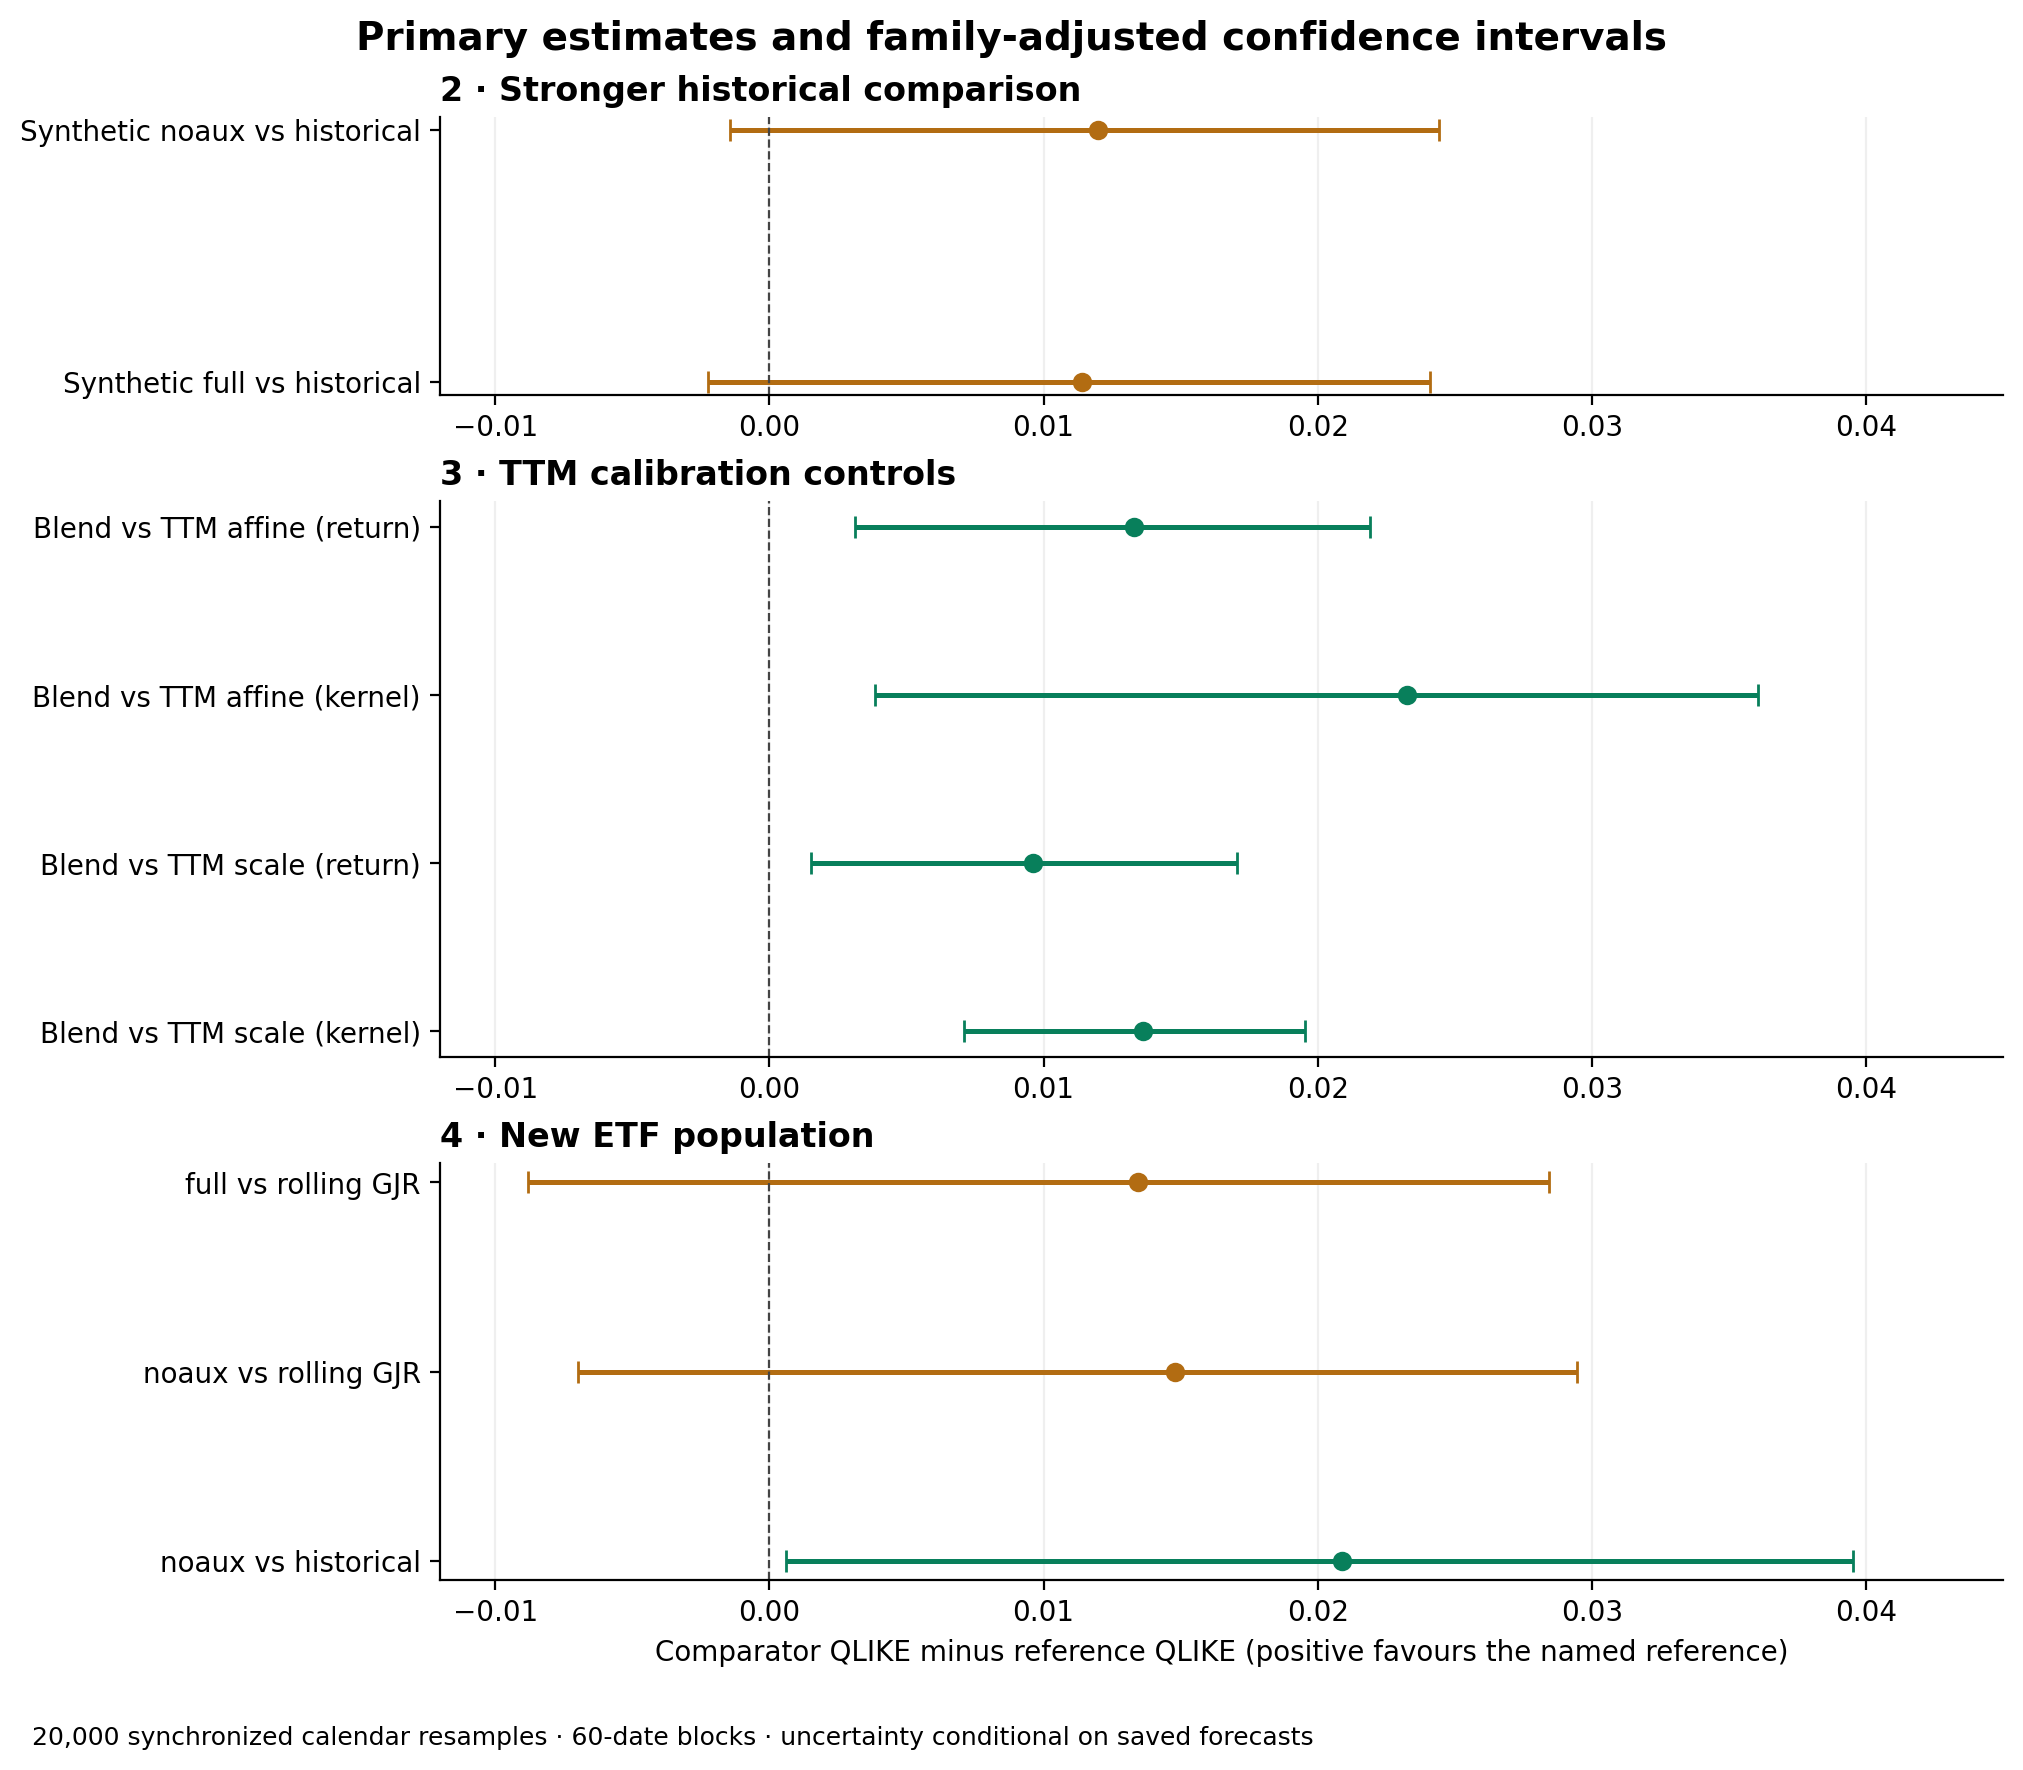
\includegraphics[width=\textwidth]{followup_primary_comparisons.png}
\caption[Primary follow-up gains and family intervals]{Saved follow-up summary: comparator-minus-reference QLIKE gains with Bonferroni family 95\% intervals, 20,000 synchronised resamples and sixty-date blocks. Green intervals are positive; amber intervals include zero. Panel labels 2--4 refer to the follow-up experiment identifiers, not dissertation chapters. Historical contrasts use 50,073 index rows per seed; calibration uses 22,026 keys at each proxy; ETFs use 22,600 rows per model/seed. Families contain two, four and three contrasts respectively. Intervals condition on saved forecasts and exclude retraining, refit re-estimation and research selection.}
\label{fig:followup-primary}
\end{figure}
\FloatBarrier

\subsection{Stronger historical comparison}

We report historical loss minus synthetic loss, so positive values favour the named synthetic procedure. The comparison retains five paired seeds, 28 markets and the original 50,073-row index mask. Neither primary family interval is wholly positive. Native and common-law NLL remain descriptive.

\begin{table}[!htbp]\centering\footnotesize
\setlength{\tabcolsep}{3pt}
\caption[Stronger historical comparison intervals]{Primary historical follow-up comparisons. Sixty-date blocks; ordinary and Bonferroni family intervals are distinct. Holm corrections apply within this family only.}
\label{tab:followup-inference-0}
\begin{tabular}{lrrrrr}
\toprule Contrast & Gain & Ordinary 95\% CI & Family 95\% CI & Holm $p$ & Markets \\
\midrule
Noaux--historical & 0.011966 & $[0.000214,0.022999]$ & $[-0.001440,0.024424]$ & 0.079196 & 20/28 \\
Full--historical & 0.011385 & $[-0.000520,0.022544]$ & $[-0.002243,0.024104]$ & 0.079196 & 19/28 \\
\bottomrule\end{tabular}\end{table}

The new historical seed QLIKE scores are 0.600664, 0.600698, 0.612527, 0.600172 and 0.596363 for seeds 8101--8105. Each retains one QLIKE-above-100 event. Both synthetic gains are positive in all paired seeds, with noaux positive in 20/28 markets and full in 19/28. The ordinary noaux interval excludes zero, but the family interval does not; marginal support therefore does not establish family-level superiority. The original mean 221.292094 and its 15,163 exceptional seed-level forecasts remain failure diagnostics, not the primary source comparison.

\FloatBarrier

\subsection{Causal TTM calibration comparisons}

The reported gain subtracts full VolPFN+TTM loss from control loss, favouring the blend when positive. Both proxies retain the same 22,026 keys and 28 markets, and all four declared contrasts pass their family rule. Raw TTM and GJR+TTM keep their earlier, separate inference.

\begin{table}[!htbp]\centering\footnotesize
\setlength{\tabcolsep}{3pt}
\caption[Causal TTM calibration comparisons intervals]{Primary causal TTM calibration comparisons. Sixty-date blocks; ordinary and Bonferroni family intervals are distinct. Holm corrections apply within this family only.}
\label{tab:followup-inference-1}
\begin{tabular}{lrrrrr}
\toprule Contrast & Gain & Ordinary 95\% CI & Family 95\% CI & Holm $p$ & Markets \\
\midrule
Affine TTM/return & 0.013311 & $[0.005432,0.020228]$ & $[0.003110,0.021917]$ & 0.001800 & 21/28 \\
Affine TTM/RK & 0.023257 & $[0.008463,0.033998]$ & $[0.003842,0.036062]$ & 0.003900 & 28/28 \\
Scale TTM/return & 0.009615 & $[0.003317,0.015530]$ & $[0.001502,0.017042]$ & 0.003900 & 20/28 \\
Scale TTM/RK & 0.013622 & $[0.008571,0.018389]$ & $[0.007095,0.019515]$ & 0.000200 & 25/28 \\
\bottomrule\end{tabular}\end{table}

Every blend seed improves over both controls at both proxies. After primary inspection, a descriptive check removes the first sixty union dates, retaining 20,414 rows. Return/RK QLIKE is 0.701348/0.627509 for the blend, 0.707067/0.641022 for raw TTM, 0.716325/0.652617 for affine TTM and 0.712339/0.642220 for scale TTM. It retains the ordering without new tests or a replacement primary population. Raw controls and the blend have different warm-up forecasts, as specified in Appendix~\ref{sec:followup-methods}.

\FloatBarrier

\subsection{Frozen external ETF comparisons}

Comparator-minus-reference loss favours the reference when positive. The fixed twenty-ETF population supplies 22,600 rows per model and seed. Only noaux--historical passes the complete primary rule; rolling-GJR family intervals both cross zero. Unverified human exposure and overlapping index-study shocks qualify this external population result.

\begin{table}[!htbp]\centering\footnotesize
\setlength{\tabcolsep}{3pt}
\caption[Frozen external ETF comparisons intervals]{Primary frozen external ETF comparisons. Sixty-date blocks; ordinary and Bonferroni family intervals are distinct. Holm corrections apply within this family only.}
\label{tab:followup-inference-2}
\begin{tabular}{lrrrrr}
\toprule Contrast & Gain & Ordinary 95\% CI & Family 95\% CI & Holm $p$ & Markets \\
\midrule
Full--Rolling GJR & 0.013460 & $[-0.004078,0.026624]$ & $[-0.008815,0.028430]$ & 0.100195 & 16/20 \\
Noaux--Rolling GJR & 0.014800 & $[-0.002427,0.027629]$ & $[-0.006986,0.029456]$ & 0.100195 & 16/20 \\
Noaux--Historical & 0.020872 & $[0.004305,0.036359]$ & $[0.000599,0.039524]$ & 0.029999 & 18/20 \\
\bottomrule\end{tabular}\end{table}

All five paired noaux--historical gains are positive: 0.018444, 0.019941, 0.031796, 0.019850 and 0.014327. Both synthetic--GJR contrasts also have positive seed means, but their primary uncertainty remains inconclusive. Eighteen of twenty ETFs favour noaux over historical and sixteen favour each synthetic model over GJR. These descriptive breadth counts are not independent market tests or an added decision gate.

\FloatBarrier

\subsection{Descriptive density endpoints}

Table~\ref{tab:followup-density} reports descriptive native and common-law NLL, with lower values preferred. Fixed synthetic and selected historical weights forecast the index panel; the ETF panel freezes these weights and retains rolling GJR's fitted mean in native scoring. Common scoring uses issued second moment under a zero-mean $t_8$ law. We construct no additional NLL hypothesis family.

\begin{table}[!htbp]\centering\small
\caption[Descriptive follow-up density losses]{Equal-market/seed mean NLL on the exact primary return masks. Historical refers to the new development-selected procedure; the original failure is separately retained in Table~\ref{tab:followup-historical}. Density endpoints are descriptive.}
\label{tab:followup-density}
\begin{tabular}{llrr}
\toprule Population & Procedure & Native NLL & Common $t_8$ NLL \\
\midrule
Indices & Full & 1.178272 & 1.184313 \\
Indices & Historical & 1.202152 & 1.187763 \\
Indices & Noaux & 1.177252 & 1.183908 \\
ETFs & Full & 1.111583 & 1.112836 \\
ETFs & Rolling GJR & 1.117771 & 1.116972 \\
ETFs & Historical & 1.138492 & 1.120480 \\
ETFs & Noaux & 1.111585 & 1.112374 \\
\bottomrule\end{tabular}\end{table}
\FloatBarrier

\subsection{Calendar-block sensitivities and complete decisions}

Table~\ref{tab:followup-sensitivity} repeats correction separately for each family's twenty- and 120-date alternatives. These are sensitivities rather than new primary tests. Historical superiority stays unresolved, all calibration contrasts remain supported, and ETF noaux--historical retains support. At twenty-date blocks the ETF--GJR adjusted probabilities both fall below 0.05, but their family intervals still cross zero. Selecting that block alone would therefore misstate the complete decision rule.

\begingroup
\small
\setlength{\tabcolsep}{4pt}
\begin{longtable}{@{}>{\raggedright\arraybackslash}p{4.5cm}rrrr@{}}
\caption[Follow-up block sensitivities]{Family-adjusted probabilities and intervals under the two alternative calendar block lengths. Gains equal the corresponding primary estimates. The two historical, four calibration and three ETF families remain separate.}\label{tab:followup-sensitivity}\\
\toprule Contrast & Block & Holm $p$ & Family 95\% interval & Support \\
\midrule\endfirsthead
\toprule Contrast & Block & Holm $p$ & Family 95\% interval & Support \\
\midrule\endhead
Index Noaux--historical & 20 & 0.079296 & $[-0.001471,0.024352]$ & No \\
Index Full--historical & 20 & 0.079296 & $[-0.002243,0.023973]$ & No \\
Index Noaux--historical & 120 & 0.052597 & $[-0.000512,0.023722]$ & No \\
Index Full--historical & 120 & 0.052597 & $[-0.001445,0.023395]$ & No \\
Affine TTM/return & 20 & 0.004650 & $[0.000800,0.023263]$ & Yes \\
Affine TTM/RK & 20 & 0.001800 & $[0.007342,0.033734]$ & Yes \\
Scale TTM/return & 20 & 0.004400 & $[0.001637,0.017376]$ & Yes \\
Scale TTM/RK & 20 & 0.000200 & $[0.008268,0.018666]$ & Yes \\
Affine TTM/return & 120 & 0.001050 & $[0.003365,0.021706]$ & Yes \\
Affine TTM/RK & 120 & 0.004300 & $[0.002809,0.037259]$ & Yes \\
Scale TTM/return & 120 & 0.004300 & $[0.001430,0.016837]$ & Yes \\
Scale TTM/RK & 120 & 0.000200 & $[0.006015,0.020360]$ & Yes \\
ETF Full--Rolling GJR & 20 & 0.030298 & $[-0.003162,0.025859]$ & No \\
ETF Noaux--Rolling GJR & 20 & 0.030298 & $[-0.001677,0.027039]$ & No \\
ETF Noaux--Historical & 20 & 0.010349 & $[0.003599,0.037269]$ & Yes \\
ETF Full--Rolling GJR & 120 & 0.129194 & $[-0.009300,0.029612]$ & No \\
ETF Noaux--Rolling GJR & 120 & 0.129194 & $[-0.007566,0.030507]$ & No \\
ETF Noaux--Historical & 120 & 0.037648 & $[0.000840,0.040642]$ & Yes \\
\bottomrule\end{longtable}
\endgroup

\subsection{Result identities and preservation}

The authoritative summaries are \path{historical_analysis_v1/}, \path{ttm_control_v1/} and \path{external_confirmation_v1/}. Each retains \path{leaderboard.csv}, \path{statistics.json}, \path{protocol.json}, \path{VERIFICATION.json} and \path{FINAL_RECEIPT.json}. The ETF directory also records execution classification, input checkpoints, original-weight checks, CPU replay and GJR causality. Source/receipt checks preserve the original inputs and distinguish serialization repair from scientific changes. Root \path{ORIGINALS_PRESERVED.json} binds consumed prior inputs; this manuscript revision separately records hashes of prior dissertation files and consumed completed results.

The original follow-up revision incorporated completed records without repeating training, forecasting, fitting or resampling. It narrowed the interpretation of historical failure and addressed the stated calibration-control gap, retaining negative and unresolved comparisons. The four prose-revision stages preserve those studies and qualifications. Implementation verification cannot establish untouched human exposure or independence from research selection.


\end{appendices}
\end{document}
